\documentclass{report}
    \usepackage{blindtext}
    %\addtokomafont{disposition}{\rmfamily}
    \usepackage[T1]{fontenc}
    \usepackage[a4paper]{geometry}
    \usepackage{comment}
    \usepackage{afterpage}
    \usepackage{xcolor}
    \usepackage{wrapfig}
    \usepackage[T1]{fontenc}
    \usepackage[scaled=0.85]{beramono}
    \usepackage{booktabs}
    \usepackage{tcolorbox}
    \usepackage{fullpage}
    \usepackage{minted}
    \usepackage{pdflscape}
    \usepackage[doublespacing]{setspace}
    \usepackage{enotez}
    \usepackage{subcaption}
    %\usepackage[singlelinecheck=off]{caption}
    \usepackage{url}
    \usepackage{verbatimbox}
    \usepackage{listings}
    \usepackage{todonotes}
    \usepackage[raggedright]{titlesec}
    \titlelabel{\thetitle.\quad} % dot after section number
    \usepackage{array,multirow,graphicx}
    \usepackage{multicol}
    \usepackage[hidelinks]{hyperref}
    \usepackage{tocloft} 
    \usepackage[english]{babel}
    \usepackage{graphicx}
    \usepackage{enumitem}
    \usepackage[section]{placeins}
    \makeatletter
    \AtBeginDocument{%
    \expandafter\renewcommand\expandafter\section\expandafter{%
    \expandafter\@fb@secFB\section
    }%
    }
    \makeatother
    \usepackage[notocbib]{apacite}
    \setcounter{tocdepth}{4}
    \usepackage{tabularx}
    \renewcommand\thesection{\arabic{section}}
    \raggedbottom
    \newcolumntype{L}[1]{>{\hsize=#1\hsize\raggedright\arraybackslash}X}%
    \newcolumntype{R}[1]{>{\hsize=#1\hsize\raggedleft\arraybackslash}X}%
    \newcolumntype{C}[2]{>{\hsize=#1\hsize\columncolor{#2}\centering\arraybackslash}X}%
    \renewcommand{\APACrefatitle}[2]{#1}
    \renewcommand{\APACrefbtitle}[2]{#1}
    \renewcommand{\APACrefbtitle}[2]{\Bem{#1}}
    \renewcommand{\APACrefaetitle}[2]{[#2]}
    \renewcommand{\APACrefbetitle}[2]{[#2]}
    \newcommand{\citepos}[1]{\citeauthor{#1}'s \citeyear{#1}}
     % this one is important for italics and stuff. 
    %from memory another may be needed. you mess with a b and c, and the 1 and 2 ... it can be done
    %\title{\emph{I am not my bipolar}: a corpus-driven discourse analysis of an online support group}
    \title{Discourse-semantics of risk in the \emph{New York Times}, 1963, 1987--2014: \\ a corpus linguistic approach}
    \author{
    Jens O. Zinn\\
    \texttt{jzinn@unimelb.edu.au}
    \and
    Daniel McDonald\\
    \texttt{mcdonaldd@unimelb.edu.au}\\
    %\multicolumn{1}{p{.7\textwidth}}{\centering\emph{University of Melbourne, Australia}}
    }

    \date{University of Melbourne, Australia\\
    ~\\
    \today}
    \begin{document}
        
    \hyphenation{under-lying language forums socia-bility dis-cur-sive pred-icator conc-ord-ancing Lee-uwen object-ivity lexico-grammar lexico-gramm-atical meta-function Esco-bedo}

    \renewcommand{\abstractname}{Abstract}

    \maketitle

\begin{abstract}

    Since the 1980s and 1990s the notion of risk has become increasingly influential in societal discourses and scholarly debate \cite{skolbekken_risk_1995}. From early work on risk and culture \cite{douglas_risk_1986,douglas_risk_2013} to the \emph{risk society} thesis \cite{beck_risk_1992,beck_world_2009,giddens_runaway_2002}, from governmentality theorists working in the tradition of Foucault \cite{dean_governmentality:_2010,omalley_risk_2012,rose_powers_1999} to modern systems theory \cite{luhmann_risk:_1993} all have built their work around the notion of risk and implicitly or explicitly refer to linguistic changes. Though this body of literature offers different explanations for the shift towards \emph{risk} and its connection to social change, to date there has been no attempt to empirically examine their relative ability to explain this change in the communication of possible harm. 

    % We will address this deficit by examining a number of claims made by different sociological risk approaches in more detail. We will utilise a corpus based approach to examine in detail how the institutional and sociocultural shift towards risk has manifested linguistically.

    To address this defecit, we conduct a corpus-based investigation of risk words in \emph{The New York Times} between 1963 and mid-2014. The investigation involves the creation of an annotated corpus of over 150,000 unqique risk tokens and their co-text. Purpose-built functions for manipulating this dataset and visualising results were created and used to investigate the corpus according to a systemic-functional conceptualisation of the transitivity and mood systems of language. This toolkit is freely available at \url{https://github.com/interrogator/corpkit}. Following the corpus interrogation, we use functional linguistics and sociological risk theory in tandem to analyse the findings. First, systemic-functional linguistics is used to link lexicogrammatical phenomena to discourse-semantic meaning of the texts. Longitudinal changes in risk language are then mapped to key events, as well as broader social movements.

    This report is accompanied by an interactive \emph{IPython Notebook} interface to our corpus and developed computational tools. Key findings from this report are stored there, as well as additional information (e.g. concordance lines, keywords, collocations), that could not be included in this report due to spatial considerations. It is available for both interactive and static viewing at \url{https://github.com/interrogator/risk}.

    \end{abstract}
    \cleardoublepage
    \pagenumbering{roman}
    %\setlength{\cftbeforetoctitleskip}{-3em}
    \singlespacing
    \tableofcontents
    \onehalfspacing
    \cleardoublepage
    \pagenumbering{arabic}

\chapter{Executive Summary}

Since the middle of the 1980s sociologists have started to argue that after WW2 significant social transformations took place in most Western industrialised societies which have manifested in a shift towards the risk semantic. Risk has become pervasive in public and scholarly debates and practices in Europe and elsewhere in the world. Following the common assumption that societal changes and language changes are closely linked, this research report aims to contribute to advancing understanding of this social shift towards risk. 

There is a wealth of literature and several sociological theories (e.g. risk society, socio-cultural, governmentality, systems theory, edgework) which offer different explanations for the shift towards risk and its connection to social change. Yet, to date there has been little attempts to empirically examine their relative ability to explain this change in the communication of possible harm. This research report addresses this deficit by:
%
\begin{enumerate}
\item Examining a number of claims made by different sociological theories and exploring linguistic changes which might not have been theoretically addressed yet. 
\item Developing a corpus based research strategy and computational research tools to examine in detail how the institutional and sociocultural shift towards risk has manifested linguistically.
\end{enumerate}
%
The study utilises The New York Times (NYT) as a case study for the US to reconstruct the growing usage of the term risk from 1987 to 2014 and examines how discourse-semantic shifts are linked to institutional and socio-cultural changes as well as socially relevant events (e.g. crises and disasters). In addition the study uses a sample of volume 1963 articles of the NYT to contrast the results with much earlier ways of risk reporting.

The investigation involves the creation of an annotated corpus of over 150,000 unique risk tokens and their co-text. Purpose-built functions for manipulating this dataset and visualising results were created and used to investigate the corpus according to a systemic functional conceptualisation of the transitivity and mood systems of language. This toolkit is freely available at \url{https://github.com/interrogator/corpkit}. 

Following the corpus interrogation, we use functional linguistics and sociological risk theory in tandem to analyse the findings. First, systemic functional linguistics is used to link lexicogrammatical phenomena to discourse-semantic meaning of the texts. Longitudinal changes in risk language are then mapped to key events, as well as broader social processes and changes.

This report is accompanied by an interactive IPython Notebook interface to our corpus and developed computational tools. Key findings from this report are stored there, as well as additional information (e.g. concordance lines, keywords, collocations), that could not be included in this report due to spatial considerations. It is available for both interactive and static viewing at \url{https://github.com/interrogator/risk}.

\section{Research Question, hypotheses} 

Most generally, the study examines \emph{how the institutionalisation of new societal practices manifest linguistically in the change of risk discourses and the use of risk language}. We also examine a number of hypotheses derived from mainstream sociological risk theorising:

\begin{enumerate}
\item Is there a shift in discourses from the positive notion of risk-taking to the negative meaning of risk?
\item Can we observe an increasing salience of the at-risk status of social groups?
\item Is there evidence for the assumption of individualised experience of risk?
\item Is there any evidence for the decreasing calculability/controllability of risk?
\item Are there any differences between different social groups in the exposure to risk?
\end{enumerate}

\section{Outcomes}

\begin{enumerate}
\item The linguistic analyses on the lexicogrammatical level and in discourse semantics give clear indications for a growing routinisation and institutionalisation of risk. We found a growing number of forms such as risk assessment or risk regulator which indicate the institutionalisation of risk practices. Decreasing arguablity and growing implicitness of risk in the clause indicated a shift from the centre to the ancillary parts of the sentence.
\item There are also clear hints that the negative notion of risk is becoming more common, indicated by a clear tendency to nominalisation but also to processes where agency is minimal (e.g. put at-risk).
\item There is a clear trend towards decreasing agency in risk processes from risking and taking risk to running risk and putting at-risk. Thus the strong norm of individual responsibility and risk-taking is accompanied by media-coverage which emphasises lacking agency in risk.
\item There is a clear increase of reporting on issues where people and particular social groups are presented as lacking control especially regarding health issues.
\item Risk reporting, in particular in the health sector, is driven by reference to scientific research supporting a rationalised approach to risk with formalised concepts such as risk factors and reference to research terms on the rise. However, expressions of control such as calculated risk are decreasing while expressions indicating the possibility of negative outcomes are increasing indicating a rise of a possibilistic notion of risk.
\item New coverage in the NYT shows a clear difference between powerful risk-takers and relatively powerless at-risk groups. The difference between the groups is sharpening over time. The powerful take more social risks while the powerless take much more substantial risks often related to illness, injury and death.
\end{enumerate}

\section{Key methodological issues}

The study demonstrates the potential for large annotated corpora to examine key claims of sociological theory about social change. It is innovative in creating a corpus comprised by annual subcorpora which allows detailed longitudinal interrogations. It takes advantage of major developments in computational linguistics\slash natural language processing such as constituency and dependency parsing. Both allow much more detailed and nuanced investigations than generally seen in CADS.

The advantages of the longitudinal analysis of one newspaper had a price, however. It is limited to a case of one genre of newscoverage. Other forms of text are not considered and might show different patterns. 

The Language processing tools developed and\slash or used in this study also have limitations. We have used the \emph{Stanford CoreNLP} NLP suite, which outputs constituency and dependency parses, rather than systemic-functional parsers. Translating the former into the latter poses a number of serious challenges. In some cases, systemic features cannot be automatically recovered from the parses, limiting the kinds of phenomena that can be automatically located and\slash or counted.

% Automated querying of lexicogrammatical patterns in of large data sets have limits due to the complexity of linguistic expressions of meaning. It necessarily has to focus on the more common patterns.

\section{Perspectives}

At the time of writing, our investigation is ongoing. In forthcoming work, we seek to:

\begin{enumerate}
\item Broaden the empirical basis integrating a growing number of US newspapers, in order to determine whether findings generated here may be generalised across mainstream U.S. print media.
\item Integrate data from newspapers of other countries (e.g. UK, Australia) into our corpus, in order to identify differences in institutional and linguistic practices across Anglophone countries.
\item Perform qualitative analysis of indivudal texts, in order to explore particular observations made in this report and their institutional contexts in more detail.
\end{enumerate}















%!TEX root = ../risk_report.tex

\chapter{Context} %: history of \emph{risk} and risk theory}

Since World War II, the term \emph{risk} has become pervasive in scholarly work and public discourse in Europe and elsewhere in the developed world (e.g. Skolbekken 1995; Zinn 2010, p. 115). Following the common assumption that societal changes and changes in language are closely linked (e.g. Luhmann 1993), the presented research contributes to a better understanding of the shift towards \emph{risk} in the media in the US. It uses The New York Times (NYT) as a case study to reconstruct the growing usage of the term \emph{risk} from 1987 to 2014 (Zinn 2010) and will examine how it is linked to institutional and socio-cultural changes as well as socially relevant events (e.g. crises and disasters). It will use a sample of 1963 articles to contrast our results with much earlier ways of risk reporting. 

There is a wealth of literature and several sociological approaches which offer different explanations for the shift towards \emph{risk} and its connection to social change. Yet, to date there has been no attempt to empirically examine their relative ability to explain this change in the communication of possible harm. We address this deficit by examining a number of claims made by different sociological risk approaches in more detail. We utilise a corpus based approach to examine in detail how the institutional and sociocultural shift towards risk has manifested linguistically.

This study aims to prove the value of the used methodology, the applicability of a corpus approach for the analysis of long term social change and the fruitfulness of combining linguistic and sociological approaches in a research design. The data and the research tools we have generated opened much more opportunities for further detailed research that we could pursue with the given resources. We will complement our study with further research in the coming years to advance our tools and refine our analysis when combining quantitative and qualitative research strategies and complement them by institutional analysis.

\section{Approaches to \emph{risk}}

Interdisciplinary risk research had been dominated by technological and psychological approaches examining public understanding and acceptance of risk. Since the 1980s social science approaches have become more influential focusing on the social shaping and construction of risk. Seminal work of Mary Douglas introduced a \emph{sociocultural approach} focussing on the social values which would determine what risks are selected and which responses are considered appropriate. Ulrich Beck introduced the most influential risk society perspective with a focus on the impact of new risks which accompany the modernisation successes such as technological advancement, increases in average wealth and health. He also showed how individualisation processes would transform a society stabilised by traditions into social forms characterised by individual decisions. Following Michel Foucault's work, a number of scholars understand risk as characterising a new way of governing societies on the basis of normative discourses of individual responsibility and improvement on the one hand and calculative technologies such as statistics and probability theory on the other. These mainstream approaches are complemented by Steven Lyng's work on \emph{edgework} as a particular form of voluntary risk taking and Niklas Luhmann's \emph{systems theory} emphasising the new ways how social complexity is managed and its impact on society.

All approaches conceptualise the link between the social representation of risks (e.g. how they are communicated, understood, and responded to) and the reality and materiality of risk. Since we do mainly only know about risk because it is communicated (whether face-to-face or different kind of print or visual media) the communication of risk is central for its social existence. But the communication of risk is only loosely coupled to its social, natural and material reality.

Since risk is future-oriented, it is always to a degree uncertain and virtual. This means it addresses a more or less known future. The tension between the uncertain possibility and the reality of risk is the build-in tension which drives debates about risk. However, this tension has been expressed in different ways. Social science theorists claim on the basis of historical analysis that the risk semantic developed and changed during long term historical processes characterised as modernisation (Bernstein, Luhmann, Giddens, Beck).

Luhmann suggests that it is a result of a new experience that is that particular gains can only be achieved when something is put at risk. He also claims that compared to societies where harm is caused by forces beyond human existence modern societies frame risks mainly as decision based. As a result, the risk semantic would become much more common while danger would lose influence since the world is increasingly considered as determined by human activities and decisions. This view is supported by Max Weber's characterisation of the modernisation processes as one of increasing rationalisation characterised by a worldview that emphasises that rational calculation rather than non-rational belief, faith (etc.) characterised the modernisation process. Not absolute knowledge but the belief in the rational manageability of the world.

Additionally, Beck and Giddens emphasise that the modern world is characterised by risks which are increasingly produced by humanity itself rather than exposed to us by the environment. That means we are observing two developments, the belief that it is mainly up to us to deal with the risks and uncertainties of our world and the reality of increasingly self-produced risks (`manufactured risks'). As a result our view of nature and environment has shifted as well, from something what has a relatively independent existence to something that is increasingly shaped by humanity (e.g. climate change).

In the \emph{governmentality perspective}, risk is not so much about the reality of risk but a specific form to manage societies. In this perspective, risk is a result of a particular way how societies govern themselves utilising calculative technologies and normative discourses of individual self-improvement and responsibility. In this perspective framing the world in terms of risk is an expression of a new form of discursive power in late modern societies. Risk is a particular discourse which informs social practices considering the future governable. Statistic probabilistic technologies are only part of these discourses though an important one.

There is little doubt that the claims about social change brought forward by different social science manifest in changing discursive practices and semantic changes. However, sociological analysis relied by now mainly on more or less anecdotal analysis of historical and semantic change. Outstanding historical work such as by Norbert Elias building on historical changes in `books of manners' is one of the most outstanding exceptions. 

Claims about historical social change made by Ulrich Beck with the most famous risk society thesis were based on general observations rather than sound empirical work. How the change towards a risk society after WW2 developed more concretely is not yet well examined.

Systematic historical studies on risk are mainly provided by researchers from the governmentality perspective (Ewald 1986; Hacking 1991; Valverde 1998; but compare: Strydom 2002; Gamson 1989). They produce valuable knowledge on the prerequisites for, and impact of, the introduction of statistics and probability calculation, and how they contribute to the governing of societies. These studies are convincing in the reconstruction of changes in institutional risk practices by specific area- or case-studies. They contribute less, however, to our understanding of how these developments compete with or complement others, and how they combine to influence a general shift in the communication, comprehension and semantics of risk in the media. 

Many theorists claim that the media are particularly influential in social risk discourse (Beck 1992), though conceptualisations like \emph{risk society} are criticized for being undifferentiated and ignoring current trends in media research (Kitzinger \& Reilly 1997, Kitzinger 1999). Media-oriented risk research mainly examines specific events or debates, such as Mad Cow Disease (BSE), genetically modified food, or international terrorism, and how news and risks are produced by the media (e.g. Allan, Adam \& Carter 2000). It does not reconstruct how \emph{risk} enters the media and how the understanding and usage of the term may have changed over time. Even the most recent special issue `Media and Risk' in the Journal of Risk Research (vol.13, no.1) ignores this important aspect. One exception is Mairal (2008). He has reconstructed how risk discourses developed over time in Spain and showed how earlier experiences and symbolical representation of risk influenced later discourses; but he did not examine semantic changes of the term \emph{risk}. 

There are strong streams of risk research on technological risk and risk assessment, health, social work and insurance. Authors such as Strydom (2002) claim that the nuclear power debates and technological risk analysis has been the major drivers for increasing concerns about risk. Similarly Beck (2009) focuses on new technologies as the driver for the growing anxiety about our future. This might underpin the different conceptualisation of risk as unexpected harm, part of statistic probabilistic calculation, or a conscious decision. Differing from Beck, first analyses have shown that in media discourses the \emph{risk} semantic is less used in articles describing new risks. Instead, a majority of articles are on health and illness and economics (Zinn 2010, p.111f.).

Many linguists are interested in overcoming the strong focus on language in discourse analysis and in incorporating social dimensions (e.g. Van Dijk 1997, Wodak \& Meyer 2001). In general, this stream of research has contributed little to the reconstruction of the historical development of discourses (Brinton 2001; Harding 2006; Carabine 2001) although many cognitive linguists examine long term semantic changes (e.g. Nerlich \& Clarke 1988, 1992, 2000; Traugott \& Dasher 2002). Regarding risk, corpus linguists have shown that sociologists' assumptions about the usage of risk are often informed by everyday life knowledge rather than systematic empirical analysis of how the term risk is actually used (Hamilton et al. 2007). \emph{Frame Semantics} has provided a detailed analysis of the available risk-frames (Fillmore \& Atkins 1992); but neither approach examines historical changes of the usage and notion of risk.

In interdisciplinary risk research there is a long-standing body of research focusing on risk communication between decision-makers and the public (e.g. Kasperson \& Stallen 1991). This research has produced valuable knowledge about how to improve the communication of risk, while media coverage is discussed from the point of view of the public's risk perception (Bennett \& Calman 1999; Slovic 2000). Some typical patterns of risk reporting are identified as well as factors which amplify and attenuate the communication of risk (Kasperson et al. 1988; Pidgeon et al. 2003; Flynn et al. 2001). However, this research contributes little to a historical perspective of how the risk semantic became pervasive in daily newspapers. 

% above reference to newspapers is quite sudden...

For risk research, the phase after WW2 has been identified as particularly crucial in the establishment of increasing debates about risk and the success of the risk semantic. Other semantics such as `threat' had its establishing phase between WW1 and WW2 during which it established as a most common term in New York Times' newspaper coverage which remains relatively stable after WW2 (Zinn XX).

The triumphal procession of risk took off before iconic events such as the Chernobyl disaster or the 9\slash 11 terrorist attacks took place. A more systematic analysis of the dynamics of the usage of the risk semantic would allow a detailed understanding of how our framing of the future in terms of risk was influenced by different forces and events. 

Originally, social science debates had been dominated by the introduction of nuclear power and the social controversies accompanying them (Douglas, Beck, Luhmann). However, the debates about DDT-based insecticides had driven the debates much earlier. The publication `The silent spring' did not impact on social science risk debates and did not stand out in the early debates of Mary Douglas and later of Niklas Luhmann and Ulrich Beck on risk. One reason might be that the semantic grounding of a risk framework had not been established at the time. 

However, there are clear indications that the risk semantic and related discourses using a risk frame became increasingly dominant during the 1980s. With our study we wanted to examine in more detail how institutional social change manifests in language. We assumed that fundamental changes such as towards a society increasingly concerned with self-produced risk would manifest in linguistic patterns even in a single genre such as print news media (similar to the Books of Manners in Norbert Elias' study). Building on an exploratory study that only counted the numbers of articles where a risk token was used at least once, Zinn 2011 provided evidence that even during a relatively short period of 1987 to 2014 we should be able to identify relatively short-term social changes within language. 


% rapid change in topic ...

% ~\ \todo[inline,color=green!40]{\noindent The following part seems a bit out of place, and repeats itself a bit.}

%\subsection{Affordances of technological innovations for risk research}

\section{Linguistic approaches to risk}

% could write this first bit in more depth if need be ...

Recently, with rapid technological developments in the digitisation of historical newspaper archives and the computational analysis of text data, it has become possible to examine long term changes in media reporting and using the media as a source for analysis of long term societal changes. Accordingly, our research takes advantage of sophisticated linguistic tools for the analysis of long-term social change---a research agenda with roots not only within the media but in the larger (social) world which effects and shifts the lexis and grammar used when reporting risk.

%Linguistic approaches to risk research to date have been from two major paradigms. First, Frame Semantics has been used to characterise risk as one or more cognitive frames\slash schemata involving a number of possible components, such as \emph{risker}, \emph{risked thing}, \emph{chance}, and \emph{positive\slash negative outcomes. This theory has then been put to use within \emph{corpus linguistic} approaches to risk, which have used large digitised datasets to understand how the risk frame(s) are typically constructed. Despite successes within this approach, it remains limited by the fact that corpora seldom provide researchers with opportunities to confirm cognitive hypotheses regarding the intentions of the writer, or the comprehension of the reader. A second key limitation is that corpus linguistic research into risk language have not been geared toward locating longitudinal change.

Central to any well-considered study of language use is a theory of language, which may either implicitly or explicitly inform the kinds of analyses being done. A number of frameworks exist for connecting lexis and grammar to functional meanings. Notable within risk research has been frame semantics, which has been used to characterise risk as one or more cognitive frames\slash schemata involving a number of possible components, such as \emph{risker}, \emph{risked thing}, \emph{chance}, and \emph{positive\slash negative outcomes}. This theory has then been put to use within \emph{corpus linguistic} approaches to risk, which have used large digitised datasets to understand how the risk frame(s) are typically constructed. Despite successes within this approach, it remains limited by the fact that corpora seldom provide researchers with opportunities to confirm cognitive hypotheses regarding the intentions of the writer, or the comprehension of the reader \cite{fillmore_toward_1992}. 

Another popular functional linguistic framework is \emph{systemic functional linguistics} \cite<see>{halliday_introduction_2004}, which conceptualises language as a \emph{sign system} that is employed by users in order to achieve \emph{social functions}. While sharing a functional view of language (as opposed to formalist views proposed by (e.g.) \citeA{chomsky_aspects_1965}), SFL is a functional-semantic theory, rather than a cognitive-semantic one. While the remarkable achievement of frame semantics is its mapping out of cognitive frames, we are largely unable to operationalise these with our dataset, as we have little information regarding the specific interactants (writers and readers) of the original texts. Moreover, cognitive understandings of text are complicated in situations where the text's author is producing the text within an institutional context, for a readership. Without downplaying the potential importance of cognitivist accounts of risk, we have instead opted here to focus on risk words as \emph{instantiations of parts of the linguistic system for the purposes of meaning-making}, rather than as a \emph{representation of the cognitive schemata that underlie our behaviour}.

A second benefit of SFL for our purposes is that it provides the most detailed functional grammar of English \cite{eggins_analysing:_2004}: when compared with frame semantics, it provides a more rigorous description of how risk can behave \emph{lexicogrammatically}---that is, in relation to both other words and grammatical features---within a clause. This makes it possible to search parsed texts in nuanced ways.

The third benefit of SFL is that it provides not only a grammar, but a a conceptualisation of the relationship between text and context. A foundational tenet of SFL, and a point of departure from other linguistic theories, is the notion that we can create a description of context based \emph{solely} on the lexicogrammatical content of the text. This is particularly suitable for us, given that our texts arrived to us abstracted from their original contexts. This context was then further obscured through the parsing process. As such, SFL provides an ability to account for discourse-semantics using corpora that other theories cannot.

In many respects, the major challenge of this project has been to find ways how to combine a linguistic analysis that goes beyond tallying the co-occurrence of lexical and grammatical features with the sociological understanding and analysis of long-term social change. As a linguistic theory that provides a taxonomy of both language and context, SFL practitioners have to date been reluctant to engage with conceptualisations of context from other traditions within the Humanities and Social Sciences. This is disappointing, especially when considering that the most common criticism of SFL is that its theory of context is heavily influenced by its theory of grammar: in SFL, context is divided into three major dimensions (Tenor, Field and Mode), which are essentially projections of a language's major grammatical systems (Mood, Transitivity, Theme).

% structure of the report?

\subsection{Aim and scope of our investigation}

Our investigation begins with a linguistic analysis of risk language in the NYT, exploring lexical and grammatical phenomena, and moving freely between different levels of abstraction (from frequency counting to concordancing of linguistic phenomena, for example). Findings from this lexicogrammatical exploration are then abstracted, according to SFL theory, to form a description of the changing discourse-semantics of risk in the NYT. This description is linked to key sociological questions, as well as discussions concerning the extent the linguistic observations can help and inform these social changes. 

We followed two major lines of analysis:

\begin{enumerate}
\item We were looking for different ways in which risk is instantiated, and how these have changed longitudinally.
\item We also looked for specific claims made by some approaches to find out whether is any indication that they are correct or require specification. 
\end{enumerate}
%
Given the vast array of changes in the behaviour of risk words uncovered, as well as limitations of time and scope, our analysis is at this stage oriented more toward a longitudinal account of language, rather than sociological theory. We outline a number of promising leads for sociological analysis, developing links between linguistic and sociological reasoning that create pathways for further research and research strategies to answer key sociological questions about social change.

\subsection{Central research questions}

There is good evidence that the risk semantic has become more common in societal practices. A direct count of articles which contain a risk token at least once showed how the dynamic of risk developed in the NYT from 1853 until today (Zinn 2011). It clearly shows how risk is mainly a phenomenon that developed a particular dynamic after WW2 while it shows at the same time that the risk semantic had been around for quite a while without a clear dynamic. This is interesting and invites more long term investigations in particular in the degrees of the usage of other terms such as `danger' and the establishment of the notion of `threat' between WW1 and WW2.

With the current study we wanted to examine in much more detail whether during a historical relatively short period from 1987 to 2014 (we used a sample of the 1963 volume to contrast with the later years) significant shifts can be observed using much more sophisticated research strategies than used in earlier corpus based approaches on the risk semantic (e.g. Hamilton et al.**).

%There are a number of social changes we were able to explore on the basis of our text corpus which are central for sociological approaches to risk. 

%\subsection{Cultural and institutional manifestation of `risk thinking'}

The most general question for our analyses may be formulated as:

\begin{quotation}
How does the institutionalisation of new societal practices manifest linguistically in the change of risk discourses and the use of risk language? 
\end{quotation}

%When institutions which deal with risk have become more common we would have more occurrences of risk institutions in media coverage. This means we would have more talk about risk management or risk assessment rather than assessing risk or managing risk since we have now the institutions of risk management or risk assessment which is a general phrase for complex but institutionalised processes of how society deals with risk.

%If knowledge about risk becomes more common it has no longer to be explained. We would no longer require explaining what the risks are. The riskiness in more implicit and less contested. It does need less support.

%When risk becomes a more common way of thinking we would expect that even when risks are low or very low, risk would still be the dominant point of reference to characterise the situation. We would report about `low risks' to characterise a situation rather than to other qualities since risk has become a dominant point of reference.

%(Obviously this paragraph could be developed a bit further but should focus on the issues we can actually measure\slash show in our analysis)

\section{Case study: \emph{The New York Times}}

We selected the NYT as a case study after careful consideration of other available resources. We aimed to find a resource that allows longitudinal analysis of long term social change with a limited number of intervening factors. We were looking for a paper which provided a high quality digitised archive and a central news institution over the centuries. 

The (London) Times and the NYT seem suitable because of their important social role within a society. They also fulfil further selection criteria such as wide circulation (not just regional), good accessibility and high data quality. However the NYT has been finally selected because of the central role of the US in the world and the prestige and clout of the NYT. The NYT is a historically central institution of media coverage (Chapman 2005) with a continuously high status and standard of coverage. It is influential, highly circulated and publicly acknowledged news media. It contains extensive coverage of both national and international developments, its digital archive covers all years since WWII and is relatively easy to access.

Available Australian Newspapers such as \emph{The Australian} or \emph{The Age} offer similar digitised archives only for recent decades and at higher cost. Long term historical analyses are much more complicated and will be pursued when we have proven our methodology.

% something missing here

The project concentrates on a single newspaper and follows a reproduction logic (Yin 1989) for four reasons: 

\begin{enumerate}
\item The `historical change of concepts' (Koselleck 2002) is so general that it can be identified even in specific newspapers though newspaper specific factors have to be considered. 
\item A detailed analysis of available newspapers archives by the CI has found that, in the US, only the Washington Post provides a comparable archive. While both show no significant differences in the general increase of the usage of the risk semantic (Zinn 2010, p. 115), access and data management has proven easier and more reliable with the NYT. 
\item The case study allows a more detailed analysis of how the change of the newspaper might have influenced the use of \emph{risk}. A collection of newspapers, as in many linguistic text corpuses would not lead to representative results but would create uncontrolled biases. Instead, the case study of a specific newspaper allows a much more detailed analysis of how change of the newspaper itself, such as a change in leadership or style of news reporting, might have influenced the use of \emph{risk}.
\item The study limits the amount of data and restricts costs without losing significant outcomes.
Originally we wanted to compare the volumes 1963, 1988, 2013 of The New York Times. We soon found out about the availability of a high quality data resource, The New York Times Annotated Corpus (\url{http://catalog.ldc.upenn.edu/LDC2008T1}9) which covers all articles published from 1987---mid-2007 and includes substantial metadata and contains 1,130,621,175 words. We complemented this data set with articles from the NYT online archive up to 2013\slash 14.
\end{enumerate}
%
In order to further validate our results, future research has been planned that will compare our results with more recent data from other US newspapers. Though in the US many newspapers are digitised the main issue is that some papers are strictly PDF while some of these PDFs have the plain text version also available. We identified major newspapers which are suitable for comparative purposes in future research. %(see below). However, we will focus on the following in a complementary study to control for newspaper-specific effects: More regional papers: St Petersburg Times\slash Tampa Bay Times (left), Denver Post (moderate), Chicago Tribune (conservative), Los Angeles Times (liberal); National oriented papers: The Wall Street Journal, Washington Post, USA Today.

\subsection{Methodology}

Given the novelty of Big Data and Big Data methods, investigations such as ours involve the development of theoretical frameworks for linking instantiated language to discourse-semantics. In our case, this involved a thorough investigation of the lexicogrammar of risk language in news journalism. In this report, we map out strategies for engaging with the systemic functional notion of experiential meaning primarily through complex querying of constituency parses. In terms of the systemic functional conceptualisation of the Mood system as a resource for making interpersonal meanings, as well as the notion of \emph{arguability}, we demonstrate novel strategies of exploiting dependency parsing provided by the Stanford CoreNLP toolkit. Though existing automated parsing generally cannot provide the level of depth necessary for full systemic annotation of language, the partial account that can be provided still proves sufficient for connecting lexicogrammar to discourse-semantics in a rigorous and systematic fashion.

As these new methods involve automated analysis via computer programming, our project also contributes to methodology via a repository of code for manipulating large and complex linguistic datasets. This repository, though designed for our particular investigation, is readily reusable by other researchers interested in how language is used as a meaning-making resource. Our methodological work is available open source at \url{https://github.com/interrogator/risk}. Documentation and code used to build and annotate the NYT corpus is also freely available there.

\subsection{Communicating results}

Emerging digital tools make it possible to display results of academic research in novel, sophisticated ways. This is crucial in Big Data studies, which may involve so much data that only a tiny fraction can be qualitatively analysed by individual (or even teams of) researchers. For risk research, the ability to package and share tools for exploring the NYT dataset allows researchers to engage in data-driven studies, which can empirically test the claims of key authors in the field.

For our investigation, we produced an \emph{IPython Notebook}, through which researchers can easily either cross-check or build upon the kinds of queries we use in our project. This goes well beyond the capacity of traditional written reports, and radically expands the potential for reproducible and transparent humanities research. In this way, our research does not stop with the publication with results: the creation of a stable database and toolkit for analysing this database is a result in and of itself. Our study is thus best considered both an investigation of risk language in the NYT and an addition to the burgeoning research area of Digital Humanities, both in terms of method for investigating data and methods for presenting results.

\section{Structure of this report}

\begin{enumerate}
\item In this chapter, we have outlined key tenets of sociological risk theory, as well as our study.
\item In the next chapter, we discuss key hypothesis in risk research in detail NYT articles.
\item In Chapter 3, we describe the process of building a text corpus from NYT articles.
\item Chapter 4 outlines the theory of language and methods used in our linguistic analysis
\item Chapter 5 details our findings from the investigation of annual subcorpora.
\item Chapter 6 details our findings from the investigation of economics, health and politics articles, with a particular emphasis on health.
\item Chapter 7 discusses these findings and relates them to sociological claims
\item Chapter 8 provides a brief research agenda and concludes.
\end{enumerate}



 % Introduction

%!TEX root = ../risk_report.tex


\section{New approaches to risk research}

Our methodology involves combining \emph{corpus assisted discourse studies} with \emph{systemic functional linguistics} in order to understand how risk words are used in the NYT, and how usage has changed within the sampled period.

\subsection{Corpus-assisted discourse studies}

Text corpora---that is, large bodies of digitised, well-structured text---are not unknown to risk researchers.

Since their work, however, enormous strides have been taken in the field of corpus-assisted discourse studies, as well as in computational fields such as natural language processing, which provide means of annotating language with grammatical information, and querying the annotated texts in complex ways.

It is also more and more feasible to build particular corpora for particular investigations, rather than relying on general corpora, comprised of diverse kinds of texts.

\subsection{Functional linguistics}

    Central to any well-considered study of language use is a theory of language, which may either implicitly or explicitly inform the kinds of analyses being done. A number of frameworks exist for connecting lexis and grammar to functional meanings. Notable within risk research has been frame semantics, which has been used to categorise different risk frames and their constituents \cite{fillmore_toward_1992}. One such framework is \emph{systemic functional linguistics} \cite<see>{halliday_introduction_2004}, which conceptualises language as a \emph{sign system} that is employed by users in order to achieve \emph{social functions}. This theory explicitly underlies our investigation.

    We use SFL for three main reasons. First, it is the most detailed functional grammar \cite{eggins_analysing:_2004}: when compared with frame semantics, it provides a more rigorous description of how risk can behave \emph{lexicogrammatically}---that is, in relation to both other words and grammatical features---within a clause. This makes it possible to search parsed texts in nuanced ways. Second, it is a functional-semantic theory, rather than a cognitive-semantic one. While the remarkable achievement of frame semantics is its mapping out of cognitive frames, we are largely unable to operationalise these with our dataset, as we have little information regarding the specific interactants (writers and readers) of the original texts. Moreover, cognitive understandings of text are complicated in situations where the text's author is producing the text within an institutional context, for a readership. Without downplaying the potential importance of cognitivist accounts of risk, we have instead opted here to focus on risk words as \emph{instantiations of parts of the linguistic system for the purposes of meaning-making}, rather than as a \emph{representation of the cognitive schemata that underlie our behaviour}.

    The third benefit of SFL is that it provides not only a grammar, but a a conceptualisation of the relationship between text and context. A foundational tenet of SFL, and a point of departure from other linguistic theories, is the notion that we can create a description of context based \emph{solely} on the lexicogrammatical content of the text. This is particularly suitable for us, given that our texts arrived to us abstracted from their original contexts. This context was then further obscured through the parsing process. As such, SFL provides an ability to account for discourse-semantics using corpora that other theories cannot.


%\section{Outcomes of the study}

%Our project makes significant contributions to both sociological theory and digital humanities methodology.


\subsection{Methodology}

Given the novelty of Big Data and Big Data methods, investigations such as ours involve the development of theoretical frameworks for linking instantiated language to discourse-semantics. In our case, this involved a thorough investigation of the lexicogrammar of risk language in news journalism. In this report, we map out strategies for engaging with the systemic functional notion of experiential meaning primarily through complex querying of constituency parses, combined with wordlists that assist with the task of dividing clauses into \emph{process types} (chiefly \emph{relational}, \emph{mental} and \emph{verbal}). In terms of the systemic functional conceptualisation of the Mood system as a resource for making interpersonal meanings, as well as the notion of \emph{arguability}, we demonstrate novel strategies of exploiting dependency parsing provided by the Stanford CoreNLP toolkit. Though existing automated parsing generally cannot provide the level of depth necessary for full systemic annotation of language, the partial account that can be provided still proves sufficient for connecting lexicogrammar to discourse-semantics in a rigorous and systemaic fashion.

As these new methods involve automated analysis via computer programming, our project also contributes to methodology via a repository of code for manipulating large and complex linguistic datasets. This repository, though designed for our particular investigation, is readily reusable by other researchers interested in how language is used as a meaning-making resource. Our methdological work is available open source at \url{https://github.com/interrogator/risk}. Documentation and code used to build and annotate the NYT corpus is also freely available there.

\subsection{Communicating results}

Emerging digital tools make it possible to display results of academic research in novel, sophisticated ways. This is crucial in Big Data studies, which may involve so much data that only a tiny fraction can be qualitatively analysed by individual (or even teams of) researchers. For risk research, the ability to package and share tools for exploring the NYT dataset allows researchers to engage in data-driven studies, which can empirically test the claims of key authors in the field.

For our investigation, we produced an IPython Notebook, through which researchers can easily either cross-check or build upon the kinds of queries we use in our project. This goes well beyond the capacity of traditional written reports, and radically expands the potential for reproducible and transparent humanities research. In this way, our research does not stop with the publication with results: the creation of a stable database and toolkit for analysing this database is a result in and of itself. Our study is thus best considered both an investigation of risk language in the NYT and an addition to the burgeoning research area of Digital Humanities, both in terms of method for investigating data and methods for presenting results.

 % Case study

%!TEX root = ../risk_book.tex


% remove?

    
%\bibliography{../../references/libwin} % Methodology

%!TEX root = ../risk_report.tex

\chapter{Case study: The New York Times, 1963--2014}

	Our investigation centred on digitised texts from \emph{New York Times} editions in 1963 and between 1987--2014. These texts (defined here as individual, complete chunks of content) are predominantly news articles, but depending on archiving practices, also included in our corpus is text-based advertising, box scores, lists, classifieds, letters to the editor, and so on. More specifically, we were interested in any  containing at least one `risk word'---any lexical item whose root is risk (\emph{risking}, \emph{risky}, \emph{riskers}, etc.) or any adjective or adverb containing this root (e.g. \emph{at-risk}, \emph{risk-laden}, \emph{no-risk}).\endnote{This was operationalised through the case-insensitive regular expression \textbf{\textbackslash brisk.*?\textbackslash b}, where \textbf{\textbackslash b} acts as a word-boundary marker.}~

	We relied on two sources for our data. The \emph{New York Times Annotated Corpus} \cite{sandhaus_new_2008} was used as the source for all articles published between 1987--2006. ProQuest was used to search for and download articles containing a risk word from 2007--2014, alongside some metadata, in HTML format. We also created a subcorpus of articles from NYT 1963 editions through optimal character recognition (OCR) of PDF documents archived by ProQuest as containing a risk word in either metadata (i.e. title, lede) or content. Due to the time-intensive nature of manual correction of OCR, a random sample of one-third (1218 texts) was selected, with paragraphs of texts containing a risk word being manually corrected by hand.

	Article text and any available metadata were extracted from this unstructured source content using \emph{Python}'s \emph{Beautiful Soup} library and added to uniquely named text files in annual subfolders. The kinds of metadata available varied according to the data source: The \emph{New York Times Annotated Corpus} provides a number of potentially valuable metadata fields, such as author, newspaper section, and subject (manually added by trained archivists). These metadata fields provided both human-readable information for use during qualitative analysis of texts, and machine-readable information that could be used to restructure the corpus in future investigations.

    We then value-added to this partially annotated corpus in three main ways. First, keywords and clusters for each article were calculated using \emph{Spindle} \cite<see>{puerto_spindle_2012} and added as metadata fields. Second, \emph{MALLET} \cite<see>{mccallum_mallet:_2002}, a topic modelling tool, used LDA to algorithmically assign `topics' to each article. The topics and their strengths were added as a metadata field. Finally, we used the \emph{Stanford CoreNLP suite} \cite<see>{manning_stanford_2014} to parse each risk token and its co-text for grammatical structure and dependencies.\endnote{As a part of an ongoing Australian Digital Humanities initiative, since the beginning of our analysis, we have been allocated resources for creating and cloud-hosting a much larger corpus. All 1.8 million articles from the \emph{New York Times Annotated Corpus} are currently being turned into an identically structured, though dramatically larger, cloud-hosted corpus. In planned future research, interrogation of this corpus will be used to determine whether trends in the behaviour of risk words were localised to the word itself, or to general stylistic/language change in the \emph{New York Times}. More details on this project are to be presented in Zinn and McDonald, forthcoming.}~

	A key strength of the methodology is that subcorpora based on article or metadata attributes can can be easily created and compared. Our interest was in creating a small set of topic-specific corpora in order to look for changes in risk word behaviour within specific fields of discourse. As a case study, we decided to focus on three broadly defined topics: \emph{economy}, \emph{health} and \emph{politics}. Librarian-added metadata concerning article topic/category (MC metadata field) was used to locate all articles tagged case-insensitive regular expressions \texttt{\textbackslash beconom.*}, \texttt{\textbackslash bhealth.*} or \texttt{\textbackslash bpolitic.*}.\endnote{We tried a number of strategies for collecting topic subcorpora, such as exploiting topic modeller and keyword metadata. Ultimately, however, we relied on the hand-classification. A limitation of the selected approach is that---an article collected in the health subcorpus was tagged with `Livestock health', for example. Similarly, article categories may be lacking: Figure \ref{fig:exfile} is tagged only with MENINGITIS, and thus is not included in our health subcorpus. More obviously, 1963 articles had not been classified this way, and thus do not feature in the three topic subcorpora.} 

	%\endnote{It would also be possible to create corpora of subtopics: from the politics domain, we could quickly find articles in which Clinton, Bush or Obama are keywords and look for differences in the behaviour of risk words for each politician. Though this seems an interesting area for future research, it was beyond our scope.}~


	\begin{table}\footnotesize \centering
    \begin{tabular}{|l|l|}
    \hline
    \textbf{Tag} & \textbf{Content}  \\ \hline
    MA    & Author(s)       \\ \hline
    MC    & Librarian-added category tags     \\ \hline
    MD    & Date of publication        \\ \hline
    MI    & Unique identifier       \\ \hline
    MK   & MALLET topic        \\ \hline
    MM    & Manually annotated topic  \\ \hline
    MP    & Section of newspaper \\ \hline
    MS    & Risk concordance line  \\ \hline
    MT    & Article title        \\ \hline
    MU    & URL for article         \\ \hline
    MZ    & Annotator comment(s)       \\ \hline
    \end{tabular}
    \caption{Metadata tags and content}
\end{table}
	
	We used some of the metadata fields to identify and remove listings (of best-selling books, plays, TV guides, etc.). Reasons for this were threefold. First, the jargon, abbreviations and non-clausal nature of listing language was not handled well by the parser. Second, list content was often repeated verbatim in multiple files, potentially skewing counts. Third, our two data sources archived listings in different ways. Listings were located by querying metadata fields in a number of ways. Files with titles such as \emph{Spare Times}, \emph{Best Sellers}, articles with keywords such as `theater', `listing', or days of the week. If a file contained only a listing, the file was removed. If a risk word appeared only within the list portion of an article, the file was deleted. If a file contained both a body and listing, only the listing was removed.

	After all data processing, we had a 150 million word corpus of nearly 150,000 articles containing a risk word published in the NYT or \url{NYT.com} in 1963, and between 1987 and mid 2014. The corpus had 29 annual subcorpora. The three subcorpora of economics, health and politics articles contained a subset of these articles. A breakdown of the size and composition of each annual subcorpus is provided in Table \ref{tab:stats}. During analysis, when conducting absolute frequency analysis, frequency counts in the 1963 subcorpus were multiplied by four, to account for the smaller sample size. Frequency counts for 2014 were multiplied by 1.37 to fill in the uncaptured period between August 18--December 31.

	\begin{table}
	    \centering
	    \footnotesize
    \begin{tabular}{p{1.5cm}|l|l|l|l|}

%\multicolumn{1}{|l}{Annual subcorpora} \\ \hline
%multicolumn{3}{c|}{RESIDUE}
\hline

\multicolumn{1}{|p{1.5cm}|}{Annual subcorpora} & \textbf{Subcorpus} & \textbf{Words} & \textbf{Articles} & \textbf{Risk words}   \\ \hline
~ & \textbf{1963} & 83,188* & 1218 &  1,584  \\ \cline{2-5}
~ & \textbf{1987} & 4,885,883 & 4,878 &  7,690  \\ \cline{2-5}
~ & \textbf{1988} & 4,834,791 & 4,703 &  7,430  \\ \cline{2-5}
~ & \textbf{1989} & 5,059,517 & 4,997 &  7,810  \\ \cline{2-5}
~ & \textbf{1990} & 5,416,187 & 5,250 &  8,244  \\ \cline{2-5}
~ & \textbf{1991} & 4,748,975 & 4,774 &  7,493  \\ \cline{2-5}
~ & \textbf{1992} & 4,923,509 & 4,818 &  7,329  \\ \cline{2-5}
~ & \textbf{1993} & 4,686,181 & 4,615 &  7,330  \\ \cline{2-5}
~ & \textbf{1994} & 4,857,729 & 4,762 &  7,384  \\ \cline{2-5}
~ & \textbf{1995} & 5,130,206 & 5,150 &  7,834  \\ \cline{2-5}
~ & \textbf{1996} & 4,969,911 & 4,773 &  7,257  \\ \cline{2-5}
~ & \textbf{1997} & 5,121,088 & 4,759 &  7,318  \\ \cline{2-5}
~ & \textbf{1998} & 6,085,810 & 5,437 &  8,351  \\ \cline{2-5}
~ & \textbf{1999} & 6,053,731 & 5,392 &  8,248  \\ \cline{2-5}
~ & \textbf{2000} & 6,472,727 & 5,717 &  8,434  \\ \cline{2-5}
~ & \textbf{2001} & 6,603,456 & 5,902 &  8,722  \\ \cline{2-5}
~ & \textbf{2002} & 6,865,631 & 6,423 & 10,288  \\ \cline{2-5}
~ & \textbf{2003} & 6,795,591 & 6,481 & 10,066  \\ \cline{2-5}
~ & \textbf{2004} & 6,776,200 & 6,215 &  9,989  \\ \cline{2-5}
~ & \textbf{2005} & 6,722,240 & 6,191 & 10,031  \\ \cline{2-5}
~ & \textbf{2006} & 6,722,592 & 6,278 &  9,965  \\ \cline{2-5}
~ & \textbf{2007} & 4,757,290** & 5,110 &  8,976  \\ \cline{2-5}
~ & \textbf{2008} & 5,300,254 & 5,384 &  9,645  \\ \cline{2-5}
~ & \textbf{2009} & 4,926,381 & 5,189 &  9,236  \\ \cline{2-5}
~ & \textbf{2010} & 5,443,658 & 5,527 &  9,560  \\ \cline{2-5}
~ & \textbf{2011} & 5,617,002 & 5,773 & 10,055  \\ \cline{2-5}
~ & \textbf{2012} & 5,366,342 & 5,302 &  9,095  \\ \cline{2-5}
~ & \textbf{2013} & 5,271,006 & 5,176 &  9,083  \\ \cline{2-5}
~ & \textbf{2014} & 3,331,580 & 3,310 &  5,635 \\ \cline{2-5}
~ & \textbf{Total} & \textbf{153,828,656} & \textbf{149,504} & \textbf{240,082} \\ \hline
\multicolumn{1}{|p{1.5cm}|}{Topic \mbox{subcorpora}} & \textbf{Subcorpus} & \textbf{Words} & \textbf{Articles} & \textbf{Risk words}   \\ \hline
~ & \textbf{Economics} & 10,489,137 & 8,286 & 32,448 \\ \cline{2-5}
~ & \textbf{Health}    & 8,524,023  & 6,944 & 36,547 \\ \cline{2-5}
~ & \textbf{Politics}  & 9,465,115  & 7,428 & 20,904 \\ \cline{2-5}
~ & \textbf{Total} & \textbf{28,478,275} & \textbf{22,658} & \textbf{89,899} \\ \cline{2-5}
\end{tabular}
    \caption{Subcorpora, their wordcount, file count and number of risk words}
    \label{tab:stats}
    \medskip % induce some separation between caption and explanatory material
\begin{minipage}{0.9\textwidth} % choose width suitably
{\footnotesize *~Only a small window of co-text---usually two sentences either side of the risk word---was preserved in this subcorpus, hence the smaller size of this sample.~\\
**~The drop in word-count here coincides with the switch from NYT Annotated Corpus to ProQuest as the data-source.\par}
\end{minipage}
\end{table}

			%\begin{table}
			%\centering
			%\small
			%\begin{tabular}{|llll|}
			%\hline
			%Economics & 10489137 & 8286 & 32448 \\ \hline
			%Health    & 8524023  & 6944 & 36547 \\ \hline
			%Politics  & 9465115  & 7428 & 20904 \\ \hline
			%\end{tabular}
			%\end{table}

\begin{figure}
\footnotesize
\begin{lstlisting}[breaklines]
<MY>92 0.14 71 0.12</M>
<MV>13 0.26 96 0.21</M>
<MG>11 0.29 3 0.20</M>
<MO>28 0.33 21 0.24</M>
<MS>One family has lost a child and others may be at risk from a deadly brain inflammation, officials warned yesterday</M>
<MJ>center: 45.444118, officials: 28.536198</M>
<MT>New Jersey Daily Briefing;Meningitis Warning Issued</M>
<MC>MENINGITIS</M>
<MU>http://query.nytimes.com/gst/fullpage.html?res=9B06EFDA1239F933A05751C1A963958260</M>
<MF>0819209.xml</M>
<MA>KELLER, SUSAN JO</M>
<MD>1995-12-30</M>
One family has lost a child and others may be at risk from a deadly brain inflammation, officials warned yesterday. Bacterial meningitis recently killed a baby who attended the Center day-care program, officials say. They are urging parents and staff at the Center to contact their doctors or a hospital emergency room.
\end{lstlisting}
\caption{Example file: NYT-1995-12-30-10.txt}
\label{fig:exfile}
\end{figure}

\section{Tools and interface used for corpus interrogation}

Special tools needed to be developed to work with the very large dataset of both raw NYT articles and parsed paragraphs containing a risk word. Given a well-established history of use within humanities and social sciences, as well as a particular strength in working with linguistic data, we developed a Python-based toolkit for querying our data and visualising query results. Our purpose-built toolkit provided the ability to quickly search each subcorpus of our data and generate useful visualisations of results. Though many parts of the toolkit were designed with more general Digital Humanities projects in mind, certain components of the toolkit were designed exclusively to aid in our particular investigation (projection of counts from 1963 and 2014; automatically stripping names and titles from U.S. politician names, etc.). The most important functions and their purpose are outlined in Table \ref{tab:pyfunc}, with a simple example of a function shown in Figure \ref{fig:code}. More detailed explanations and demonstrations are provided at \url{http://nbviewer.ipython.org/github/interrogator/risk/blob/master/risk.ipynb}; the repository of code itself is available via \emph{GitHub} (\url{https://github.com/interrogator/risk}), where it can freely be downloaded, or duplicated and modified.

\begin{table}[h!]
\small
\centering
\begin{tabularx}{0.5\textwidth}{|l|X|} \hline

\textbf{Function name} &  \textbf{Purpose}     \\ \hline
\texttt{interrogator()}  &  interrogate parsed corpora          \\ \hline
\texttt{dependencies()}  &  interrogate parsed corpora for dependency info (presented later)          \\ \hline
\texttt{plotter()}       &  visualise \texttt{interrogator()} results  \\ \hline
\texttt{table()}          &  return \texttt{plotter()} results as table  \\ \hline
\texttt{quickview()}     &  view \texttt{interrogator()} results       \\ \hline
\texttt{tally()}       &  get total frequencies for \texttt{interrogator()} results       \\ \hline
\texttt{surgeon()}       &  edit \texttt{interrogator()} results       \\ \hline
\texttt{merger()}       &  merge \texttt{interrogator()} results       \\ \hline
\texttt{conc()}          &  complex concordancing of subcorpora  \\ \hline
\texttt{keywords()}          &  get keywords and ngrams from corpus\slash subcorpus\slash concordance lines  \\ \hline
\texttt{collocates()}          &  get collocates from corpus\slash subcorpus\slash concordance lines \\ \hline
\texttt{quicktree()}          &  visually represent a parse tree  \\ \hline
\texttt{searchtree()}          &  search a parse tree with a Tregex query  \\ \hline
\end{tabularx}
\caption{Python functions developed for our investigation}
\label{tab:pyfunc}
\end{table}

\begin{figure}
\centering
\begin{minipage}[c]{.75\textwidth}
\centering
\begin{minted}[fontsize=\small,linenos=true]{python}
def collocates(data, nbest = 30, window = 5):
    """Feed this a csv file generated with conc() and get collocations"""
    import nltk
    from nltk import collocations
    from nltk.collocations import BigramCollocationFinder
    import re
    f = open(data)
    raw = f.read()
    bad, good = re.compile(r'Entire sentences \(n=[0-9]+\):').split(raw)
    good = unicode(good.lower(), 'utf-8', errors = 'ignore')
    sent_tokenizer=nltk.data.load('tokenizers/punkt/english.pickle')
    sents = sent_tokenizer.tokenize(good)
    tokenized_sents = [nltk.word_tokenize(i) for i in sents]
    allwords = []
    # for each sentence,
    for sent in tokenized_sents:
    # for each word,
        for word in sent:
        # make a list of all words
            allwords.append(word)
    bigram_measures = nltk.collocations.BigramAssocMeasures()
    finder = BigramCollocationFinder.from_words(allwords, window_size=window)
    ignored_words = nltk.corpus.stopwords.words('english')
    # anything containing letter or number
    regex = r'[A-Za-z0-9]'
    # the n't token
    nonot = r'n\'t'
    # lots of conditions!
    finder.apply_word_filter(lambda w: len(w) < 2 or w.lower() in \
        ignored_words or not re.match(regex, w) or re.match(nonot, w))
    finder.apply_freq_filter(2)
    results = sorted(finder.nbest(bigram_measures.raw_freq, nbest))
    listversion = []
    for index, thecollocation in enumerate(results):
        aslist = [index, thecollocation[0], thecollocation[1]]
        listversion.append(aslist)
    return listversion
\end{minted}
\caption{Python code to find collocates in concordance results}
\label{fig:code}
\end{minipage}
\end{figure}


Finally, we developed an IPython Notebook based interface for using these functions to investigate the NYT corpus (also available via our GitHub URL above). This served not only as our main platform for interrogating the dataset, but also as a means of dynamically disseminating results without being limited by considerations of space. In being open-source, and in explicitly showing the exact queries used to generate findings, the Notebook ensures both reproducibility and transparency of the entirety of our investigation. At the same time, it provides a framework for sophisticated corpus-assisted discourse analysis using cutting-edge digital research tools. Researchers are encouraged to run the Notebook in conjunction with this report, so that they can generate and manipulate our key findings as they see fit.


% \begin{table}
% \centering
% \tiny
% 
% \begin{tabularx}{1.0\textwidth}{|llllllllllllllllllllllllllllll|}
% \hline
% 
% \textbf{Subcorpus}          & \textbf{1963}  & \textbf{1987}    & \textbf{1988}    & \textbf{1989}    & \textbf{1990}    & \textbf{1991}    & \textbf{1992}    & \textbf{1993}    & \textbf{1994}    & \textbf{1995}    & \textbf{1996}    & \textbf{1997}    & \textbf{1998}    & \textbf{1999}    & \textbf{2000}    & \textbf{2001}    & \textbf{2002}    & \textbf{2003}    & \textbf{2004}    & \textbf{2005}    & \textbf{2006}    & \textbf{2007}    & \textbf{2008}    & \textbf{2009}    & \textbf{2010}    & \textbf{2011}    & \textbf{2012}    & \textbf{2013}    & \textbf{2014}    \\ \hline
% \textbf{Wordcount}     & 83188 & 4885883 & 4834791 & 5059517 & 5416187 & 4748975 & 4923509 & 4686181 & 4857729 & 5130206 & 4969911 & 5121088 & 6085810 & 6053731 & 6472727 & 6603456 & 6865631 & 6795591 & 6776200 & 6722240 & 6722592 & 4757290 & 5300254 & 4926381 & 5443658 & 5617002 & 5366342 & 5271006 & 3331580 \\
% \textbf{Article count} & 1218  & 4878    & 4703    & 4997    & 5250    & 4774    & 4818    & 4615    & 4762    & 5150    & 4773    & 4759    & 5437    & 5392    & 5717    & 5902    & 6423    & 6481    & 6215    & 6191    & 6278    & 5110    & 5384    & 5189    & 5527    & 5773    & 5302    & 5176    & 3310    \\
% \textbf{Risk words}    & 1584  & 7690    & 7430    & 7810    & 8244    & 7493    & 7329    & 7330    & 7384    & 7834    & 7257    & 7318    & 8351    & 8248    & 8434    & 8722    & 10288   & 10066   & 9989    & 10031   & 9965    & 8976    & 9645    & 9236    & 9560    & 10055   & 9095    & 9083    & 5635    \\
% \hline
% \end{tabularx}
%     \caption{Subcorpora their wordcount, file count and risk token count}
% \end{table}
% 
% 	%Figure charting articles, words, risk tokens by year here \label{fig:stats}
		
%\bibliography{../references/libwin} % Findings: annual

\chapter{\emph{Risk} in health articles in the NYT}

    This chapter is currently being prepared for publication, and cannot be included here. See: \\ 

    Zinn, J. O. \& McDonald, D. (2015). \emph{Changing Discourses of Risk and Health-Risk: a corpus analysis of the usage of risk language in The New York Times}. Chamberlain, M. (ed.) 2015/6: Medicine, Discourse, Power and Risk. Routledge

%!TEX root = ../risk_report.tex

\chapter{Findings} \label{chap:findings}

    Findings are organised according to the formulation of areas of interest as questions. These questions progress from general frequency counting (Q1), through experiential meanings (Qs 2--7), to risk as modifier (Qs 8 \& 9) and finally to arguability (Q10). Discussion of the general significance of individual findings is also presented in this section, as the Discussion section synergises all findings to explain the discourse-semantics of risk.

    \vspace{5mm}
    \noindent\begin{tcolorbox}[colback=yellow!5,colframe=yellow!40!black,title=Summary: an example]
    \parbox{1\textwidth}{%
    Summaries of each major finding will be presented in highlighted text boxes.}
    \end{tcolorbox}
    \vspace{5mm}

    \noindent An \emph{IPython Notebook} interface for navigating the corpus \cite<see>{mckinney_python_2012}, as well as the code used to interrogate it and the findings we produced, is available online: \url{https://github.com/interrogator/risk}. A non-interactive version is available at \url{http://nbviewer.ipython.org/github/interrogator/risk/blob/master/risk.ipynb}. This Notebook does not suffer from spatial limitations, and thus contains additional information, including the exact Tregex queries used in interrogations, as well as complete lists of the concordance lines discussed only briefly here. Tools and results from other kinds of corpus linguistic analysis, such as keywording and collocation, are also available there, but have not been described here.

\section{How frequently do risk words appear?} \FloatBarrier

    %We successfully located a number of lexicogrammatical sites of change within clauses containing a risk word. 

    The first point of interest was the overall frequency of risk words in the NYT (Figure \ref{fig:relative_frequency_of_risk_words}) and the distribution of risk words by word class (nominal, verbal, adjectival\slash adverbial), absent any consideration of surrounding grammar (see Figure \ref{fig:wordclasses}). In terms of the relative frequency of risk words, we note a general upward trend, with a number of peaks and troughs worthy of further investigation. In terms of word classes of risk, we found that not only are nominal forms by far the most common in the NYT, but that it is nominal risk words that vary the most in frequency, with the other categories remaining more or less stable. Interestingly, in the span for which we have no data (1964--1986), adjectival forms overtake verbal forms of risk in frequency.

    %Using our reference corpus, we checked to see whether nominals were becoming more frequent within the NYT more generally.

    \noindent
    \begin{figure}[htb!]
    \centering
    \begin{minipage}{.45\textwidth}
    \centering
    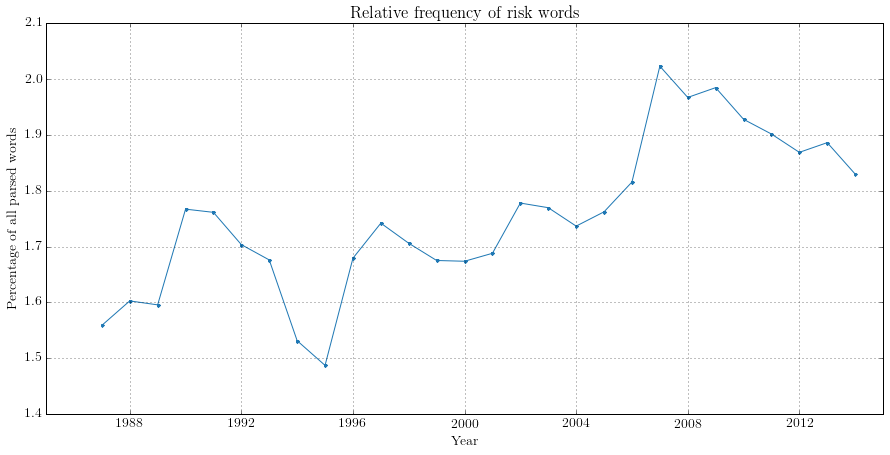
\includegraphics[width=.95\textwidth]{../images/relative_frequency_of_risk_words.png}
    \caption{Relative frequency of risk words}
    \label{fig:relative_frequency_of_risk_words}
    \end{minipage}%
    \begin{minipage}{.55\textwidth}
    \centering
    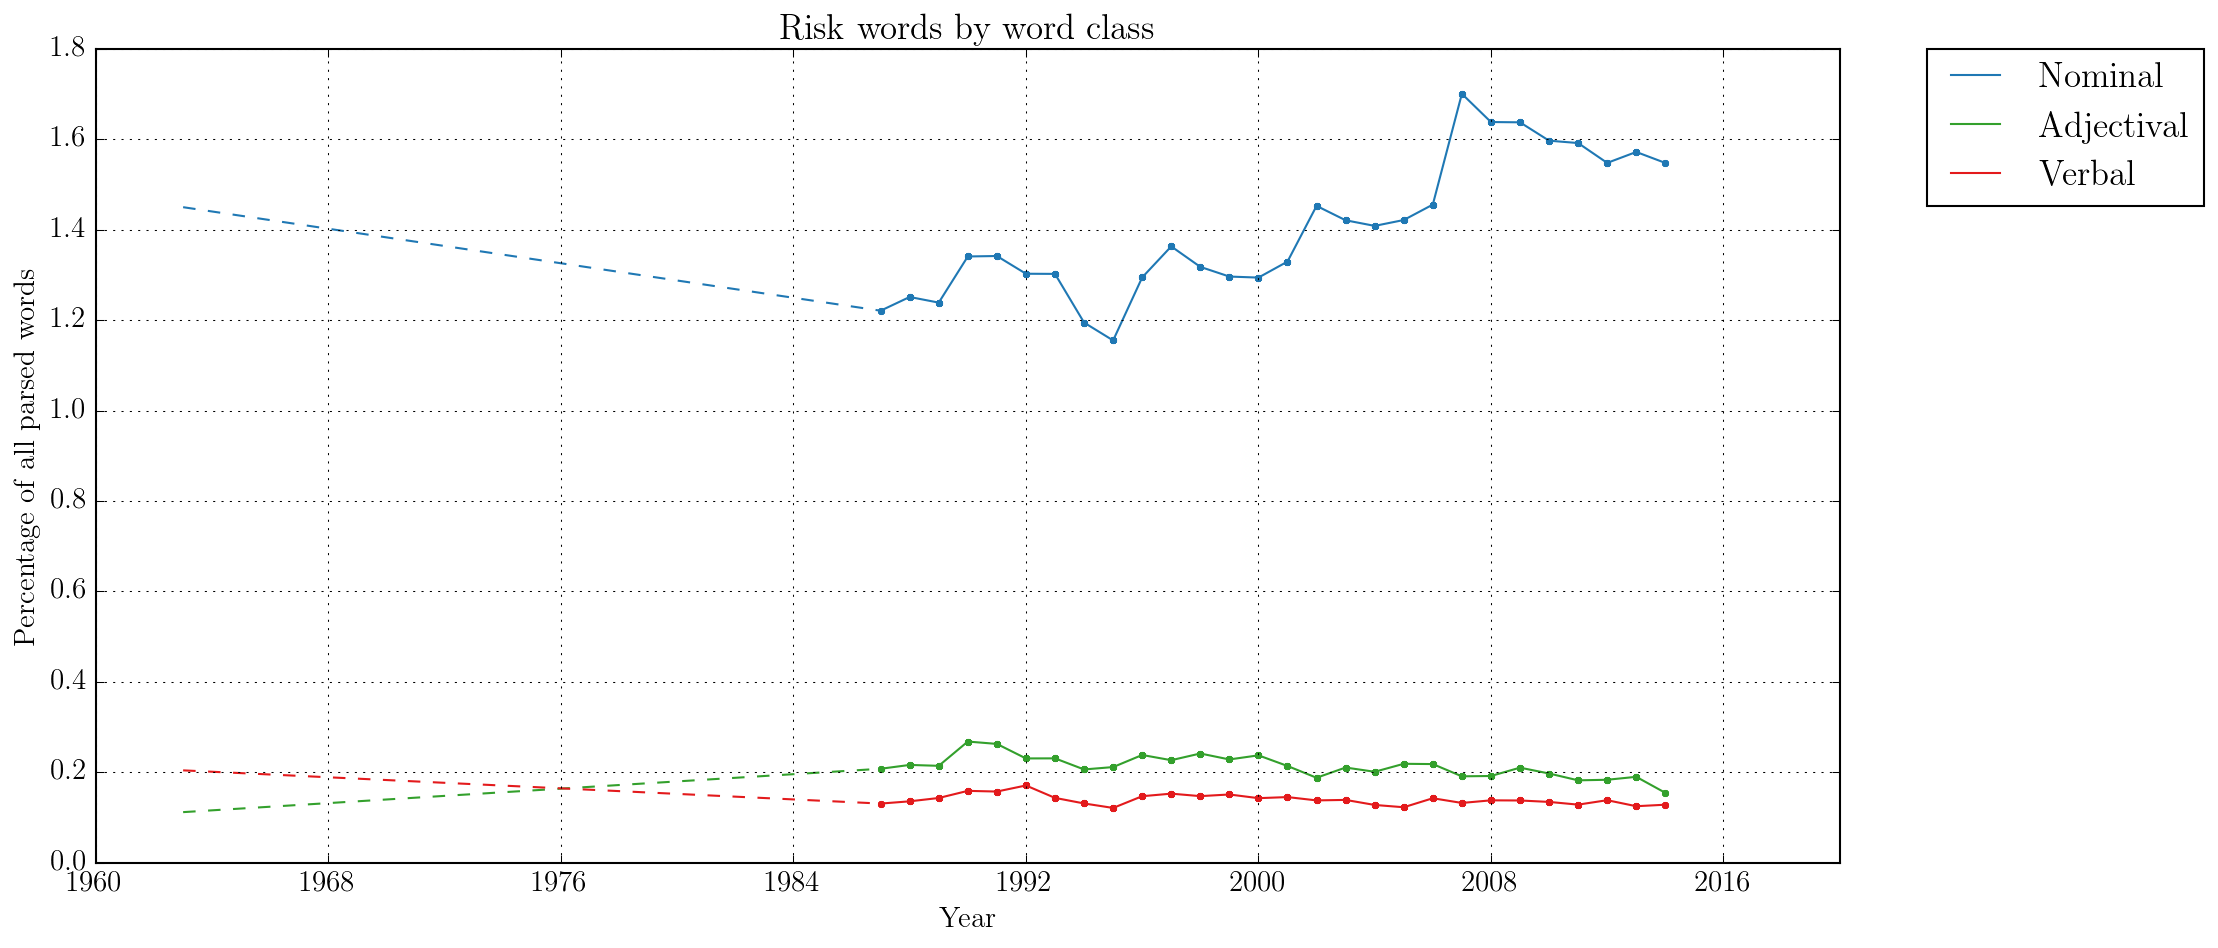
\includegraphics[width=.95\textwidth]{../images/risk_words_by_word_class.png}
    \caption{Relative frequency by word class}
    \label{fig:wordclasses}
    \end{minipage}
    \end{figure}

    %\begin{figure}[htb!]
    %\centering
    %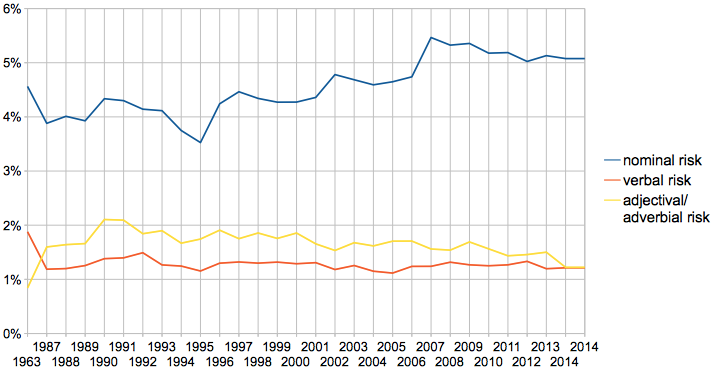
\includegraphics[width=0.75\textwidth]{../images/relwordclass.png}
    %\caption{Risk words by word class as percentage of all parsed words}
    %\label{fig:relwordclass}
    %\end{figure}

    %FUNCTIONAL CATEGORISATION?

    We compared this against the relative frequencies of nominal, verbal and adjectival\slash adverbial lexical items in the corpus as a whole, in order to account for any trends toward nominalisation in our dataset more generally (Figure \ref{fig:wordclasses}). This showed that even when compared to potential trends toward nominalisation generally, nominal risks are still on an inbound trajectory.

    These initial findings guided the rest of the investigation: particular attention was paid to nominal risks, as these were the site of the most longitudinal change. That said, these categories provide merely a categorisation of the formal features of risk words. Functionally, things are substantially more complicated: \emph{running a risk}, for example, while featuring a nominal risk, is in reality a risk process; similarly, though risk is nominal in \emph{risk management}, risk is nominal, it functions as a modifier, rather than a participant.

    A similar question is the number of unique risk words appearing per year. Figure \ref{fig:diffriskwords} demonstrates that there does appear to be a general increase in the relative number of risk words over time.\endnote{1963 is excluded from analysis here, as poor quality OCR created a number of non-word results such as \emph{risks-wnrk}, \emph{risks.North} and \emph{risks.With}.}

    \begin{figure}[htb!]
    \centering
    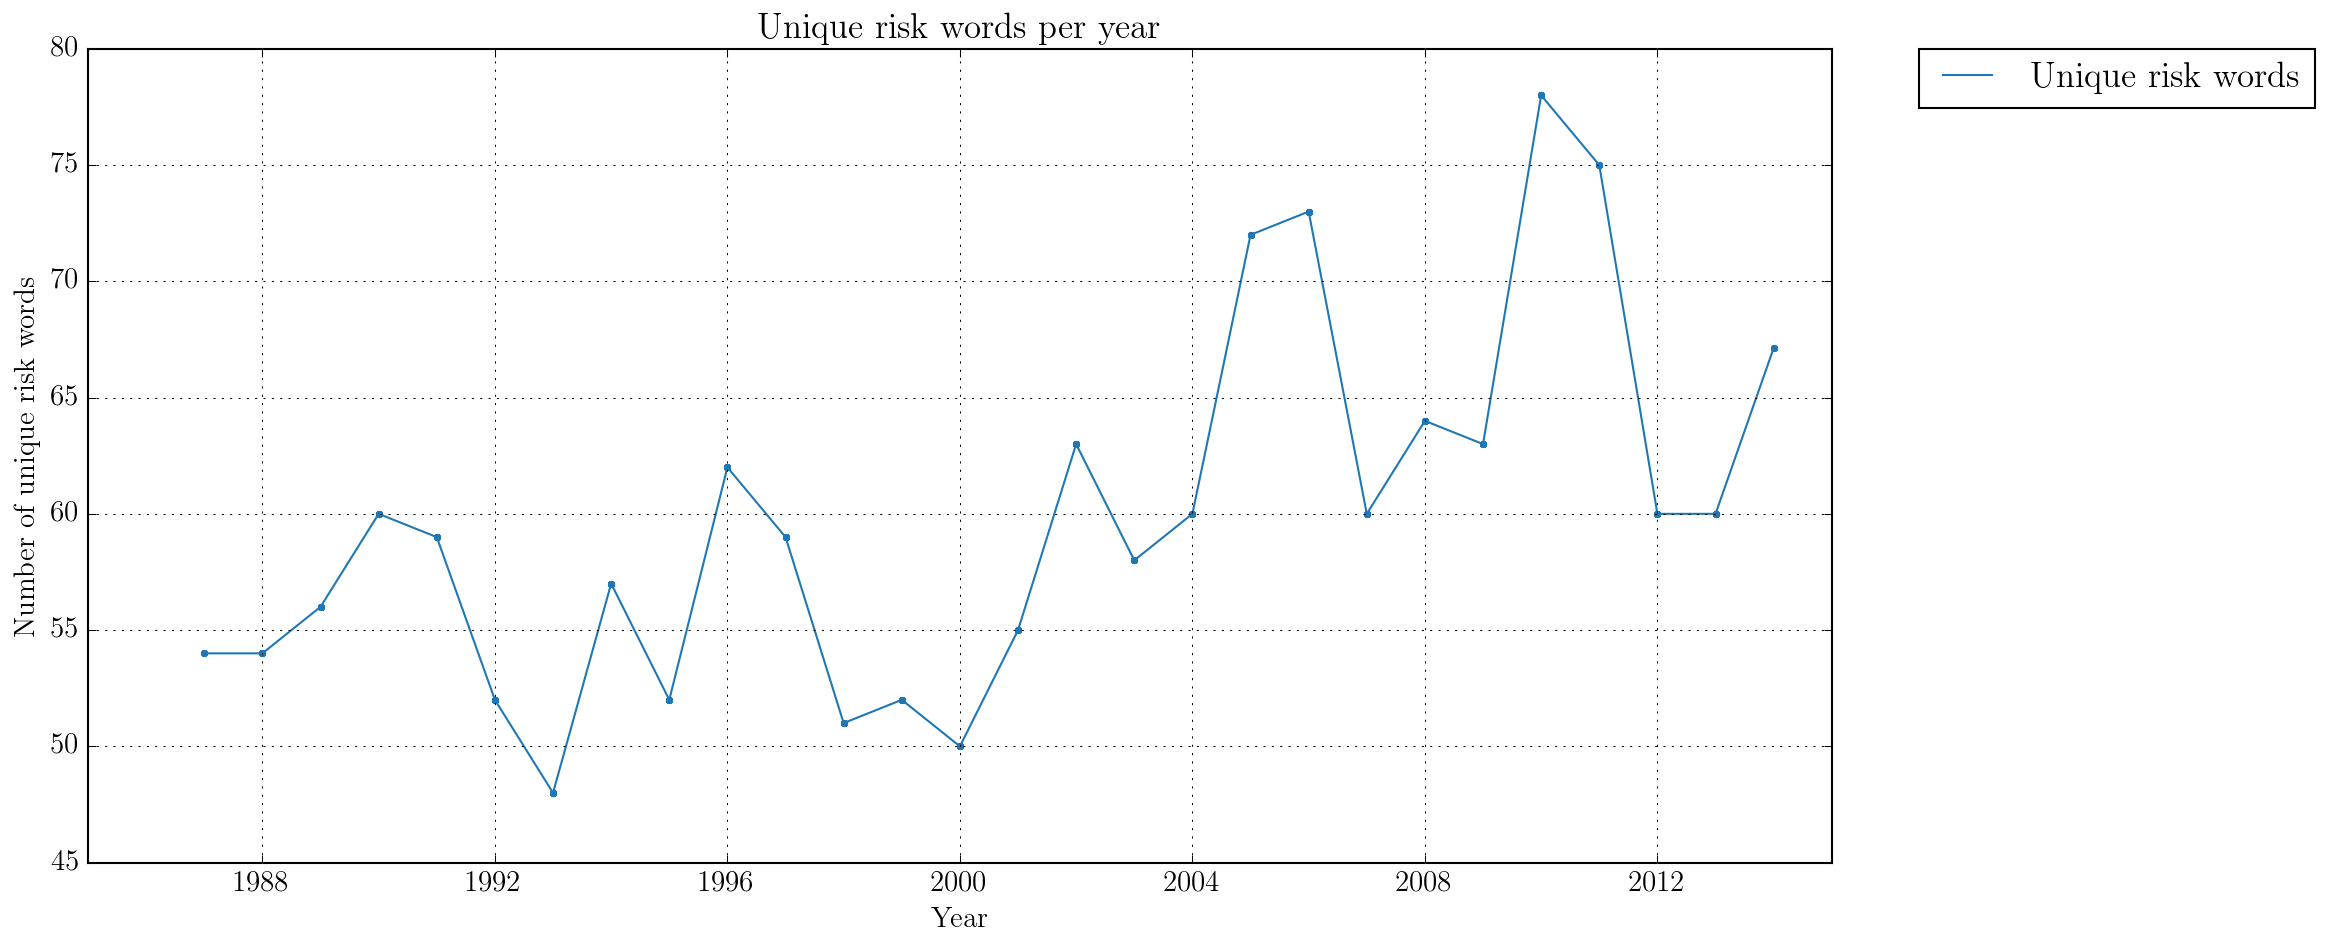
\includegraphics[width=0.7\textwidth]{../images/unique_risk_words_per_year.png}
    \caption{Unique risk words}
    \label{fig:diffriskwords}
    \end{figure}

    \vspace{5mm}\noindent\begin{tcolorbox}[colback=yellow!5,colframe=yellow!40!black,title=Summary: frequency of risk words]
    \parbox{1\textwidth}{%
    Risk words appear to be increasing in relative frequency, with modest increases in the number of unique risk words per year.}
    \end{tcolorbox}
    \vspace{5mm}



\section{Which experiential roles do risk words occupy?} \FloatBarrier

    In a systemic-functional conceptualisation of the experiential metafunction of language, risk words may take the form of a Participant (\emph{The risk was there}), Process (\emph{I risked it}) or a Modifier (\emph{a risky encounter}). Though these pattern to some extent with word classes (e.g. \emph{participant = noun, process = verb, modifier = adjective}), word classes on the whole are a poor indication of functional role, especially in genres such as print news journalism,  which rely heavily on nominalisation and grammatical metaphor to pack large amounts of experiential information into each clause. As shown in Table \ref{tab:class_and_role}, for example, nominal risks commonly perform Modifier functions, and adjectival functions often perform Participant functions.

    \begin{table}
    \small
    \centering
    \begin{tabular}{|l|l|l|}
    \hline
    \textbf{Example}       & \textbf{Word class}     & \textbf{Experiential role}     \\ \hline
    It was risky  & Adjective  &  Participant   \\ \hline
    There was a risking & Noun  &  Nominalised process   \\ \hline
    Risk management  & Noun & Modifier   \\ \hline
    \end{tabular}
    \caption{Key differences between word class and experiential role}
    \label{tab:class_and_role}
    \end{table}

    Using Stanford CoreNLP's dependency parses, we counted the frequency of risk words within these three functional roles (Figure \ref{fig:funcrole}). In line with the results from word-class based searching, we find that risk as a Process is declining in use. Risk as Modifier, patterning in part with adjectival risk, appears to be increasing. That said, we can also see here the affordances of a functional grammar in corpus assisted discourse research: in this case, much richer evidence of changing usage of risk can be found through an understanding of its semantic function rather than its word class alone.

    % today comprises a larger proportion of risk Participants than in earlier samples. 

    There is a clear trend toward using risk as a Participant.
    Nominalisation of risk is in and of itself evidence of a greater implicitness of risk, as the core function of nominalisation is to pack more information into the clause. Nominalisation thus reflects 


    In terms of experiential meaning

    Nominalisation is also closely tied to arguability. This link is discussed in Section \ref{sect:arguability}.

    %``From studies comparing identical and fraternal twins, it is estimated that genetic factors account for 40 to 60 percent of the variation in the risk for addiction.''

    %That was just one day after Richard S. Fuld Jr. , Lehman 's chief executive , announced a new strategy that he said would `` accomplish a significant de-risking of our balance sheet , '' in part by putting risky assets into a new company it would spin off to shareholders next year .

    % `` Ambac has consistently emphasized that in this period of extreme uncertainty in the capital markets , the de-risking and de-leveraging of our balance sheet is our highest priority , '' David W. Wallis , the chief executive , said in a news release .

    \begin{figure}[htb!]
    \centering
    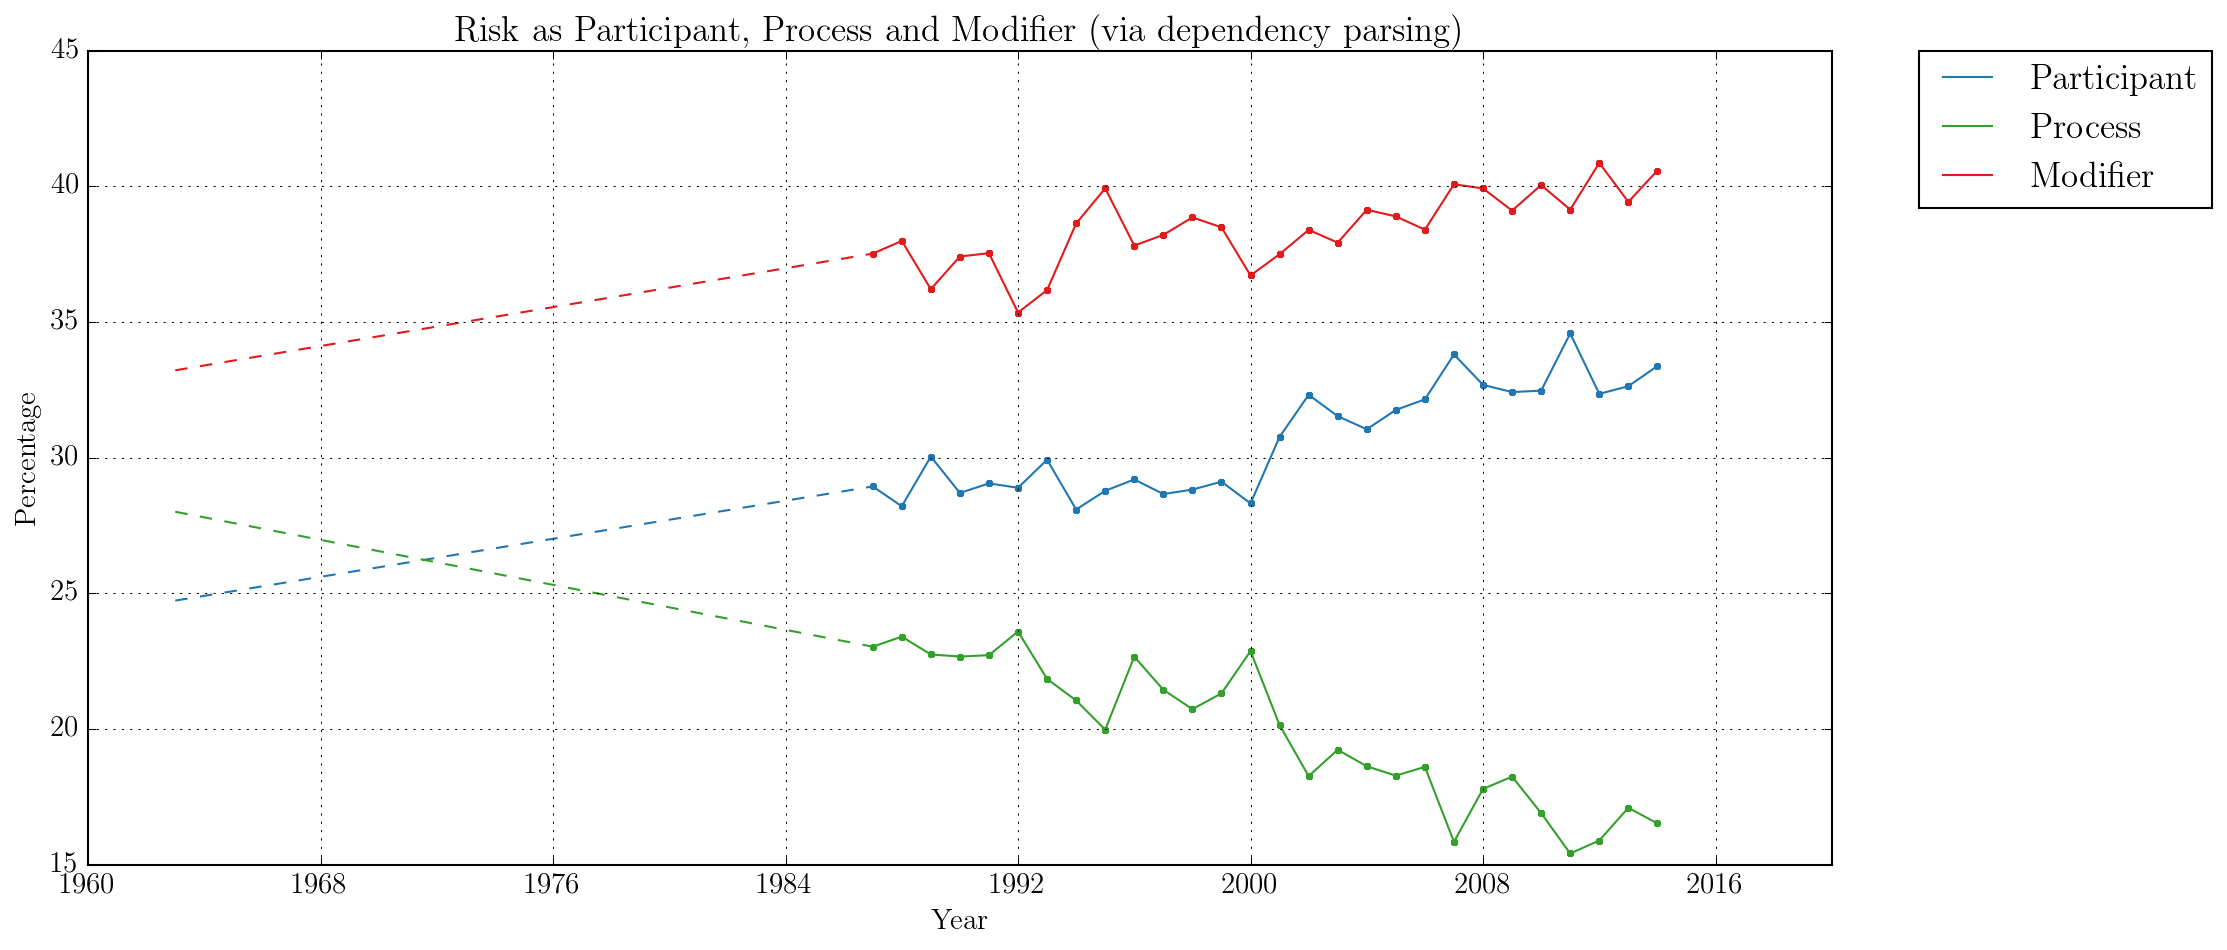
\includegraphics[width=0.7\textwidth]{../images/risk-as-participant-process-and-modifier-via-dependency-parsing.png}
    \caption{Experiential roles of risk words}
    \label{fig:funcrole}
    \end{figure}

    %~\ \todo[inline,color=yellow!40]{\noindent More discussion here, perhaps, as well as the above chart as relative frequencies. I may also have to account for risk within prepositional phrases here.}
    
    %only when the risk word forms the head of these groups, rather than a dependent/modifier (e.g. \emph{a risky decision}).

    \vspace{5mm}\noindent\begin{tcolorbox}[colback=yellow!5,colframe=yellow!40!black,title=Summary: experiential function of risk words]
    \parbox{1\textwidth}{%
    Risk as a process is declining in use, and has been overtaken in frequency by risk as a participant.}
    \end{tcolorbox}
    \vspace{5mm}

\section{Is risk more commonly in the position of experiential subject or experiential object?} \FloatBarrier

    Risk as a participant may take the form of an experiential subject or an experiential object. Our first area of interest was the proportion of each, with respect to general trends in the NYT. As shown in Figure \ref{fig:bestexpsubjobj}, risk is more commonly an object than a subject. It is also apparent that risk as experiential subject is on an static trajectory, while risk as experiential object is inbound. The significance of this is discussed in more depth in Section \ref{sect:arguability}.

    \begin{figure}[htb!]
    \centering
    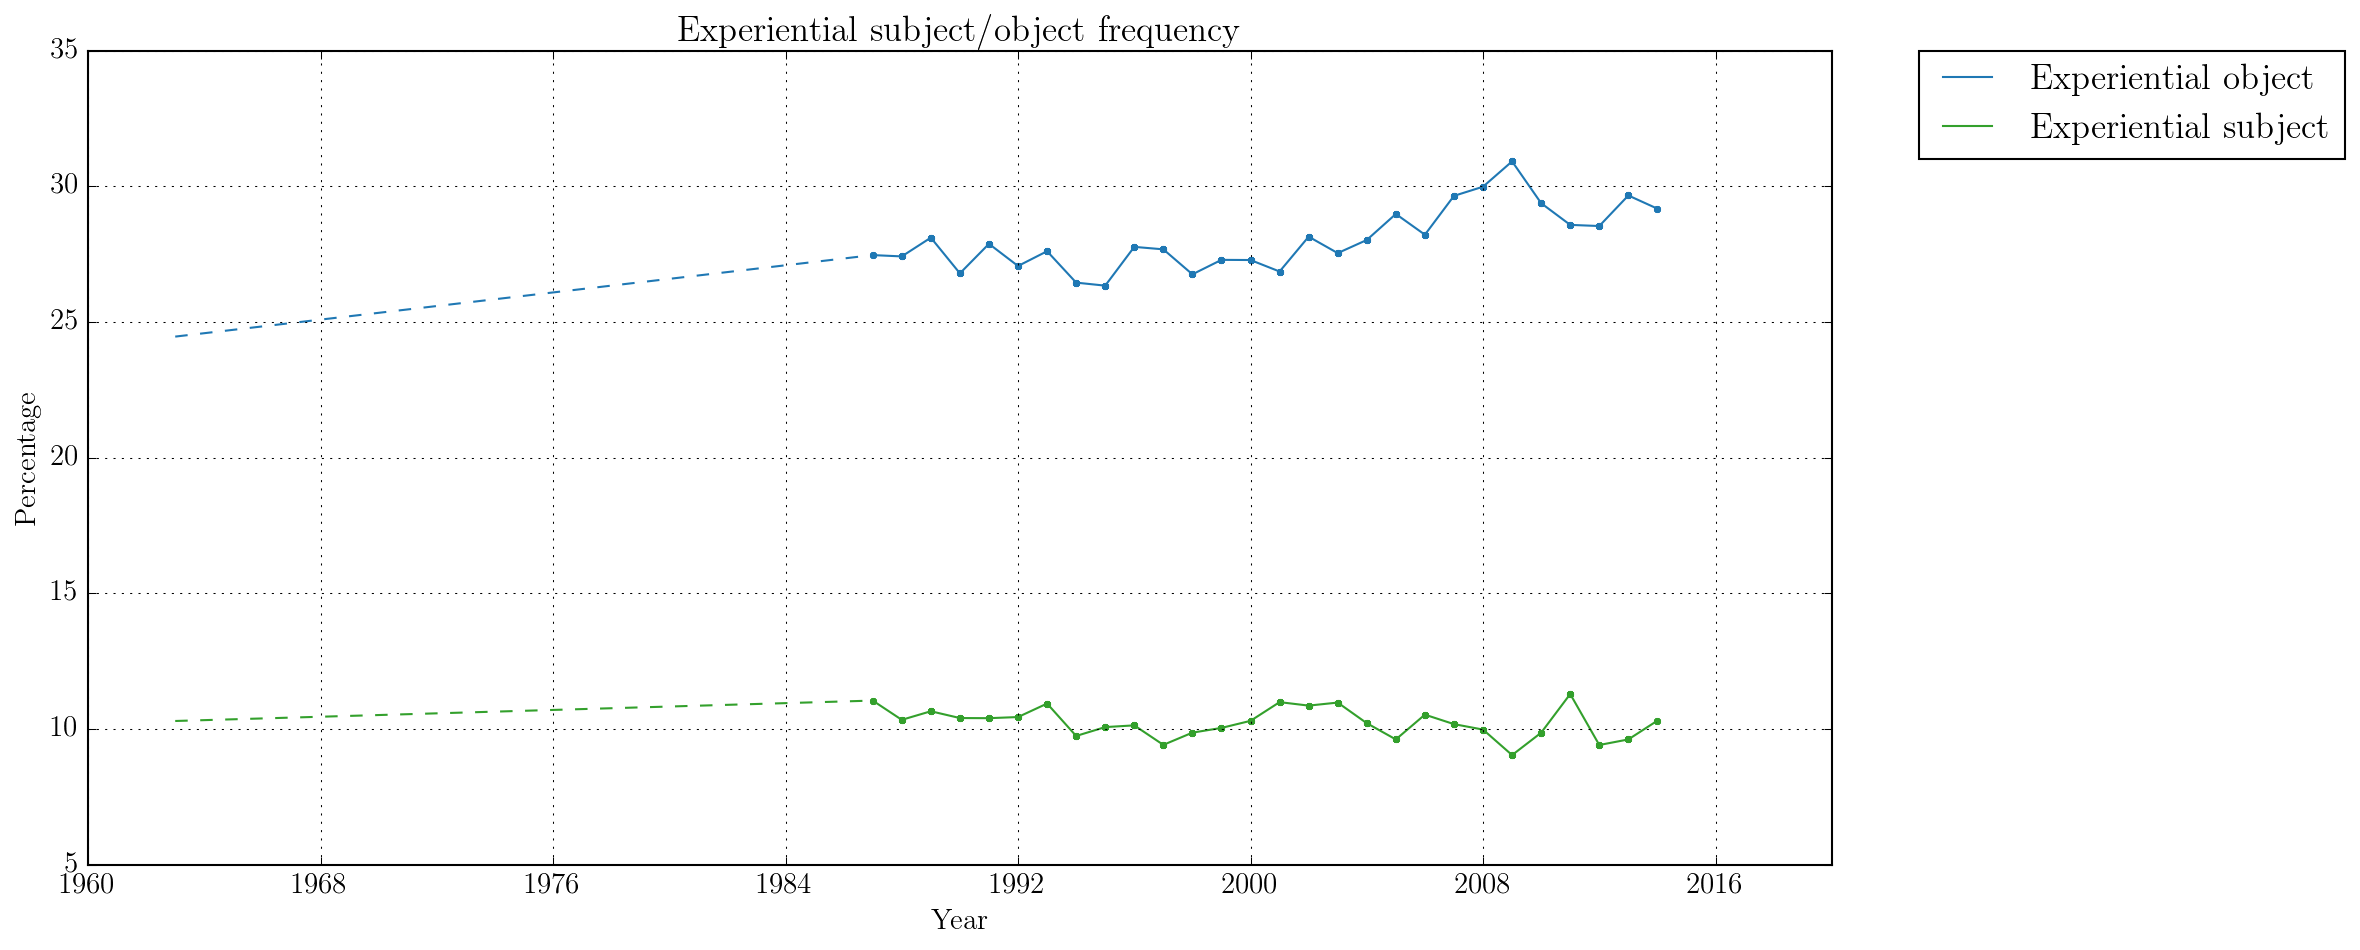
\includegraphics[width=0.75\textwidth]{../images/experiential_subject_object_frequency.png}
    \caption{Risk as experiential subject and object as percentage of all risk roles}
    \label{fig:bestexpsubjobj}
    \end{figure}
    %

    \begin{table}[tb]\footnotesize
    \centering
    \addvbuffer[12pt 8pt]{\begin{tabularx}{0.75\textwidth}{|X|X|}
    \hline
    \textbf{As subject} & \textbf{As object} \\ \hline
    \textit{But the most prevalent \textbf{risk} for the average traveler to Peru is the high altitude of the Andes}   & \textit{The company has resolved accounting problems, he said, and stabilized profit margins, while new management has reduced the company's \textbf{risks}}  \\ \hline
    \textit{The \textbf{risk} would be that the stock would recover during the period that the investor was out of the stock}   & \textit{But an empty village is a big \textbf{risk}.}  \\ \hline
    \textit{But the \textbf{risk}, though very small, that a man facing execution could win a new trial raises the question why this rule has proved so hard to follow}   & \textit{They said there was only a little \textbf{risk}, and now he 's not with us anymore} \\ \hline
    \end{tabularx}}
    \caption{Examples of risk as experiential subject and object in 2001}
    \label{tab:subj_conc}
    \end{table}



    \vspace{5mm}\noindent\begin{tcolorbox}[colback=yellow!5,colframe=yellow!40!black,title=Summary: risk as experiential subject\slash object]
    \parbox{1\textwidth}{%
    Risk is more often an experiential object than an experiential subject. The gap has widened considerably over time.}
    \end{tcolorbox}
    \vspace{5mm}



\section{What processes are involved when risk is a participant?} \FloatBarrier

    We then wanted to determine the most common processes in which risk as a participant is involved. Tables \ref{tab:subj} and \ref{tab:obj} show the top twenty processes for risk as experiential subject and object, taking passivisation into account.\endnote{\emph{Take} and \emph{run} are removed from the object column here, as \emph{take risk} and \emph{run risk} are considered risk processes.}~

    % this below doesn't count agent as an experiential subject, and it should! also copula

    \begin{table}[htb!]
    \centering
    \addvbuffer[12pt 8pt]{\begin{minipage}{.35\textwidth}
    \small
    \begin{tabularx}{1.0\textwidth}{|>{\raggedright}X|l|}
    \hline
    \textbf{Processes when risk is experiential subject} & \textbf{Total} \\ \hline
    be                                      & 8954  \\ \hline
    increase                                & 460   \\ \hline
    outweigh                                & 278   \\ \hline
    rise                                    & 269   \\ \hline
    say                                     & 222   \\ \hline
    come                                    & 201   \\ \hline
    remain                                  & 192   \\ \hline
    go                                      & 190   \\ \hline
    have                                    & 179   \\ \hline
    make                                    & 148   \\ \hline
    seem                                    & 148   \\ \hline
    involve                                 & 145   \\ \hline
    grow                                    & 133   \\ \hline
    exist                                   & 127   \\ \hline
    take                                    & 121   \\ \hline
    become                                  & 120   \\ \hline
    lose                                    & 120   \\ \hline
    include                                 & 113   \\ \hline
    appear                                  & 111   \\ \hline
    pay                                  & 100   \\ \hline
    \end{tabularx}
    \caption{Processes when risk is \mbox{experiential} subject}
    \label{tab:subj}
    \end{minipage}} \hspace{1cm} % This must go next to `\end{minipage}`
    \addvbuffer[12pt 8pt]{\begin{minipage}{.35\textwidth}
    \small
    \begin{tabularx}{1.0\textwidth}{|>{\raggedright}X|l|}
    \hline
    \textbf{Processes when risk is experiential object} & \textbf{Total} \\ \hline
    %take                                             & 11459 \\ \hline
    reduce                                           & 5609  \\ \hline
    pose                                             & 4179  \\ \hline
    increase                                         & 4063  \\ \hline
    %run                                              & 3506  \\ \hline
    have                                             & 2879  \\ \hline
    carry                                            & 2115  \\ \hline
    face                                             & 1477  \\ \hline
    raise                                            & 1115  \\ \hline
    minimize                                         & 1009  \\ \hline
    assess                                           & 841   \\ \hline
    create                                           & 731   \\ \hline
    outweigh                                         & 704   \\ \hline
    avoid                                            & 683   \\ \hline
    present                                          & 619   \\ \hline
    assume                                           & 593   \\ \hline
    consider                                         & 588   \\ \hline
    see                                              & 563   \\ \hline
    understand                                       & 493   \\ \hline
    accept                                           & 492   \\ \hline
    weigh                                        & 473   \\ \hline
    eliminate                                        & 450   \\ \hline
    
    \end{tabularx}
    \caption{Processes when risk is experiential object}
    \label{tab:obj}
    \end{minipage}}
    \end{table}

    Interesting here is the dominance of processes seeking to quantify risk. Also salient is the presence of a large set of mental processes (seem, appear, assess, understand, accept). 

    Future research is planned to divide processes with risk participants into the systemic functional conceptualisation of process types. Potentially, we could determine whether or not risks are shifting to or from mental to material.

    \vspace{5mm}\noindent\begin{tcolorbox}[colback=yellow!5,colframe=yellow!40!black,title=Summary: processes with risk participants]
    \parbox{1\textwidth}{%
    When risk is a participant, quantification is often at the centre of the experiential meaning. The high proportion of mental processes highlights a portrayal of risks as perceived.}
    \end{tcolorbox}
    \vspace{5mm}

\section{How are participant risks modified?} \FloatBarrier

    Most commonly, risk as a participant is modified through adjectival pre-head modification or post-head modification with a subordinate clause or prepositional phrase. Ignoring the distinction between subject and object risk, and collapsing pre-head and post-head kinds of modification, Tables \ref{tab:prehead} and \ref{tab:posthead} show the most common pre- and post-head modifiers of risk as a participant.

    \begin{table}%[htb!]
    \centering
    \addvbuffer[12pt 8pt]{\begin{minipage}{0.35\textwidth}
    \raggedleft
    \small
    \begin{tabular}{|l|l|}
    \hline
    \textbf{Pre-head modifier}     & \textbf{Total} \\ \hline
    high         & 4753  \\ \hline
    great        & 3444  \\ \hline
    big          & 1672  \\ \hline
    political    & 1520  \\ \hline
    potential    & 1340  \\ \hline
    financial    & 1164  \\ \hline
    low          & 1056  \\ \hline
    more         & 1051  \\ \hline
    significant  & 1003  \\ \hline
    serious      & 935   \\ \hline
    real         & 869   \\ \hline
    little       & 761   \\ \hline
    own          & 713   \\ \hline
    substantial  & 547   \\ \hline
    less         & 541   \\ \hline
    such         & 514   \\ \hline
    calculated   & 469   \\ \hline
    considerable & 463   \\ \hline
    possible     & 458   \\ \hline
    other        & 423   \\ \hline
    \end{tabular}
    \caption{Pre-head modification of participant risk}
    \label{tab:prehead}
    \end{minipage}} \hspace{1cm}% This must go next to `\end{minipage}`
    \addvbuffer[12pt 8pt]{\begin{minipage}{0.35\textwidth}
    \raggedright
    \small
    \begin{tabular}{|l|l|}
    \hline
    \textbf{Post-head modifier} & \textbf{Total} \\ \hline
    cancer             & 2344  \\ \hline
    disease            & 1777  \\ \hline
    attack             & 1597  \\ \hline
    death              & 1025  \\ \hline
    injury             & 823   \\ \hline
    infection          & 811   \\ \hline
    loss               & 408   \\ \hline
    war                & 391   \\ \hline
    failure            & 383   \\ \hline
    inflation          & 368   \\ \hline
    problem            & 346   \\ \hline
    default            & 336   \\ \hline
    stroke             & 325   \\ \hline
    complication       & 288   \\ \hline
    damage             & 251   \\ \hline
    transmission       & 248   \\ \hline
    harm               & 244   \\ \hline
    aid                & 227   \\ \hline
    recession          & 217   \\ \hline
    accident           & 208   \\ \hline
    \end{tabular}
    \caption{Pre-head modification of participant risk}
    \label{tab:posthead}
    \end{minipage}}
    \end{table}

    Some of these modifiers are undergoing longitudinal trajectory change. As can be seen in Figure \ref{fig:reladjrisk}, \emph{calculated risk} has an outbound trajectory, decreasing steadily. The large number of occurrences projected for 1963, however, is partially the result of the 1962 Broadway play by the same name. Of course, the choice of name for the production may also serve as evidence for the salience of the construction in the earlier samples.  \emph{Potential risk}, on the other hand, is increasing in frequency. Also interesting is the spike in the \emph{high risk} construction between 2002--2004. %REDO PROJECTION FOR 1963...

    Concordancing reveals links to particular events. \emph{High risk}, peaking in 2004, is asociated with the outbreak of the H5N1 avian flu outbreak. %Interestingly, however, many concordance examples deal only with strains common in the USA:

    \begin{enumerate}   [before=\itshape,font=\normalfont] \setlength\itemsep{0em} \small
    \item Mr. Johannessen said health care providers had a moral obligation to ensure -- through direct questions and, if necessary, medical records -- that people who asked for flu shots were at high risk. 
    \item Dr. Anthony S. Fauci, director of the National Institute of Allergy and Infectious Diseases, said that nearly 90 million Americans had a high risk of catching flu, with half of that number usually seeking vaccinations. 
    \item Nearly 90 million Americans are at high risk to contract a potentially fatal case of influenza. 
    \item Dr. Hinds said his county had about 90,000 people at high risk for flu. 
    \end{enumerate}
    %

    % http://en.wikipedia.org/wiki/Global_spread_of_H5N1_in_2004
    
    % ./tregex.sh -t -o -w '/(?i).?\brisk.?/ >># (NP < (JJ < /high/))' data/nyt/trees/years/2004 > jens_2004_high_risk.txt

    \begin{figure}%[htb!]
    \centering
    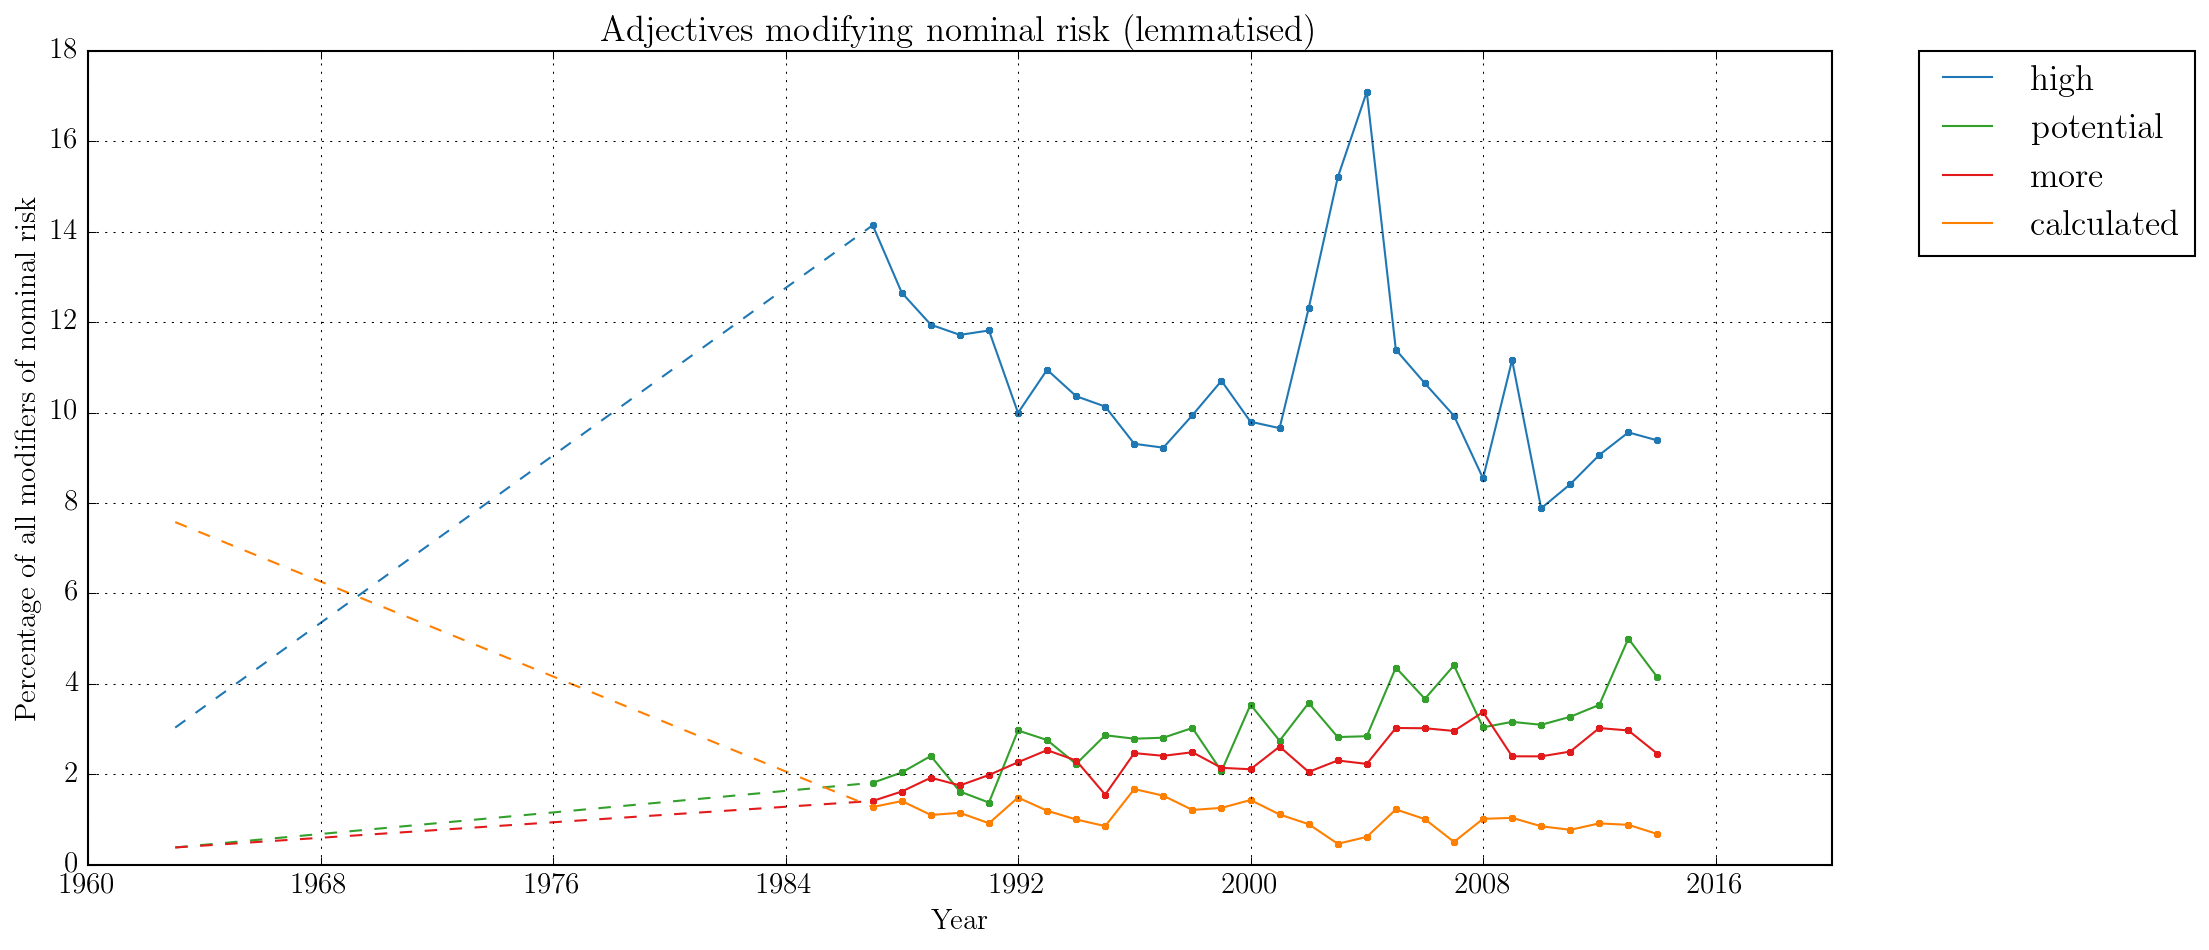
\includegraphics[width=0.75\textwidth]{../images/adjectives_modifying_nominal_risk_(lemmatised).png}
    \caption{Selected modifiers of participant risk as percentage of all risk modifiers}
    \label{fig:reladjrisk}
    \end{figure}

    %~\ \todo[inline,color=yellow!40]{\noindent Significance of this?}

    \vspace{5mm}\noindent\begin{tcolorbox}[colback=yellow!5,colframe=yellow!40!black,title=Summary: modifiers of risk as participant]
    \parbox{1\textwidth}{%
    \emph{Calculated risk} has been overtaken by \emph{potential risk} in overall frequency. \emph{High-risk} spikes in frequency in references to H5N1.}
    \end{tcolorbox}
    \vspace{5mm}


\section{What kinds of risk processes are there, and what are their relative frequencies?} \FloatBarrier

    Our second area of interest within the transitivity system is risk as a process. Within the corpus, we located five distinct risk processes. First, risk alone may be a process (\emph{I won't risk it}). Second and third are \emph{running risk} and \emph{taking risk}---\emph{process--range} configurations, where the verbal component is largely shorn of meaning, and with meaning conveyed primarily in the nominal in object position \cite{halliday_introduction_2004}. Fourth is \emph{putting somebody/something at risk}, which involves an obligatory nominal object argument and a prepositional-phrase complement. Finally, we have

    Other phrases sit on the cusp as recognisable risk processes: \emph{to carry risk}, for example, is frequent in the data, but we have not included it because we feel that the semantic burden of this process still lies in \emph{carry} (unlike \emph{pose} in \emph{to pose risk}).

    \begin{figure}[htb!]
    \centering
    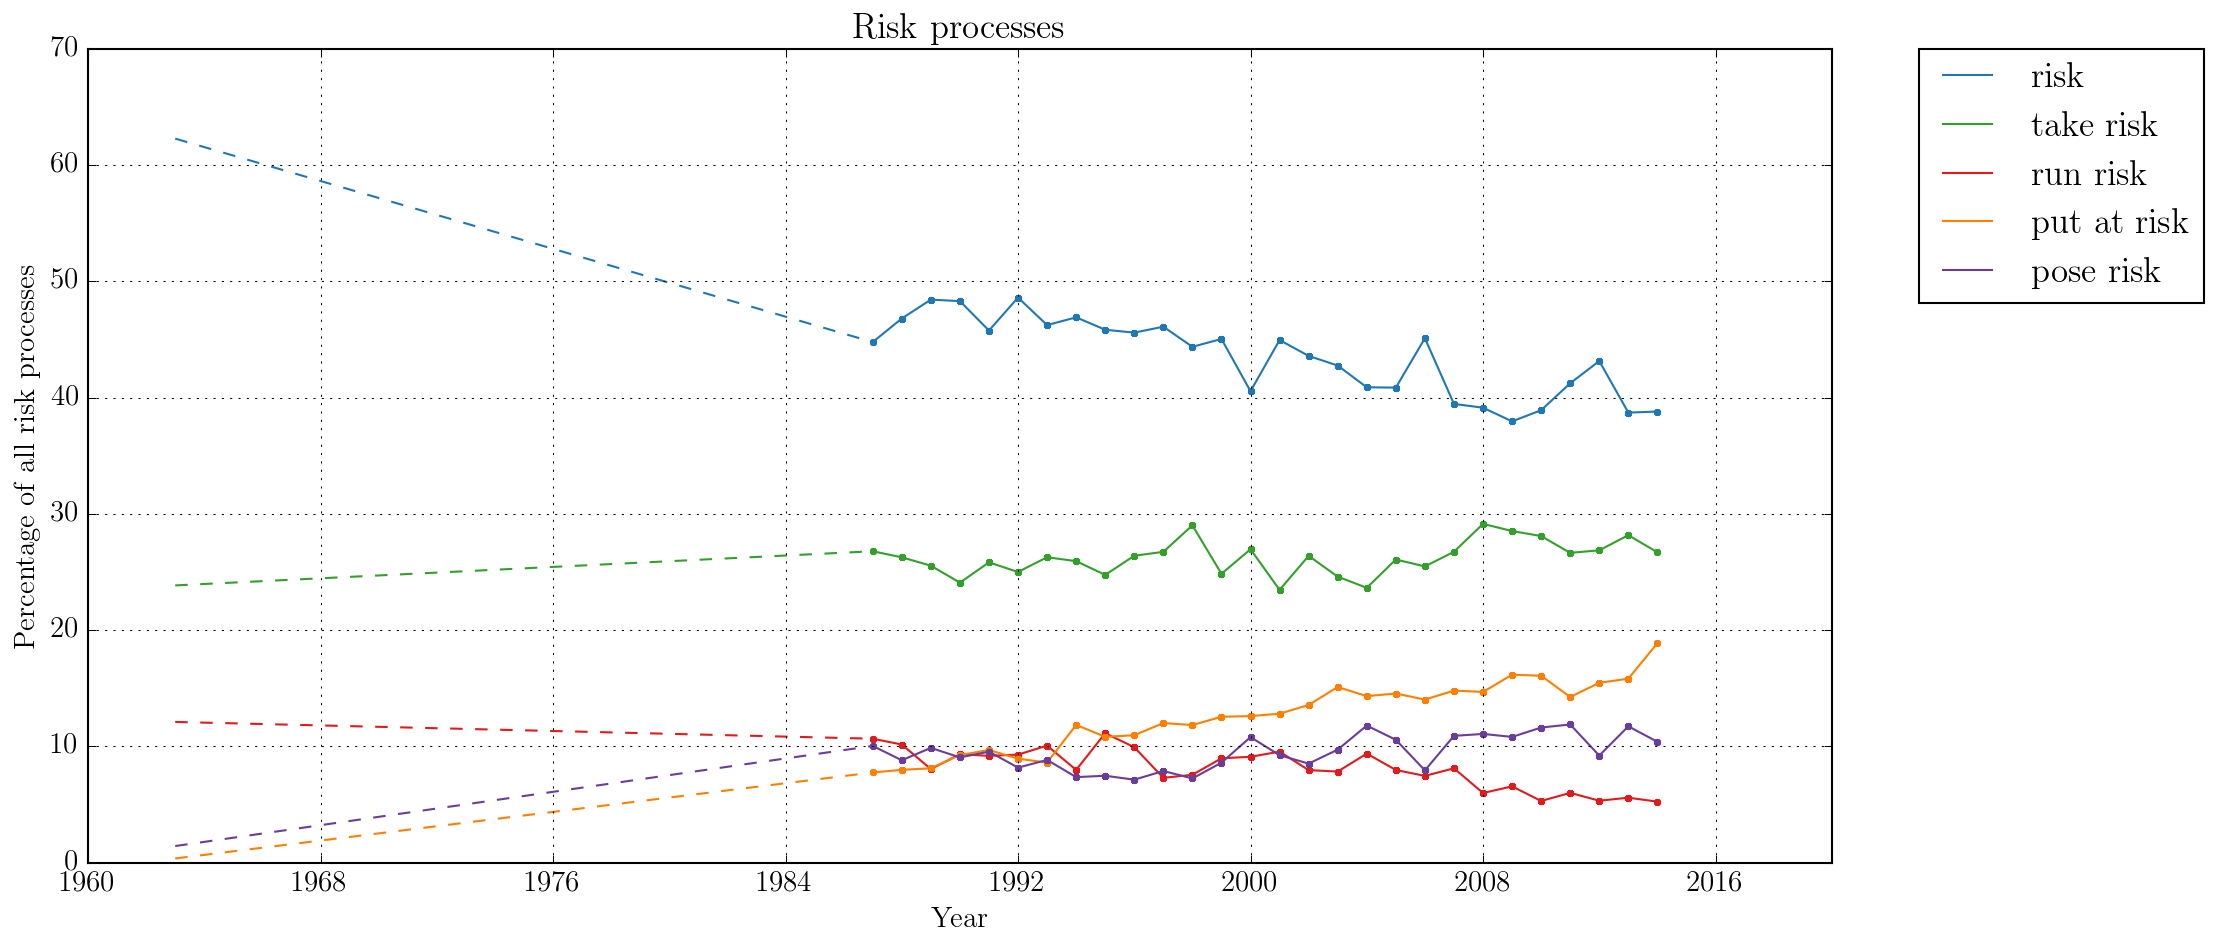
\includegraphics[width=0.75\textwidth]{../images/risk_processes.png}
    \caption{Risk processes as percentage of all parsed processes}
    \label{fig:riskprocesses}
    \end{figure}
    %
    Our first interest is the overall frequency of these five risk processes. 
    %From Figure \ref{fig:riskprocesses}, we concluded that risk processes generally are on an static\slash slightly outbound trajectory, with a notable decrease in frequency between the 1963--1987 samples.
    Figure \ref{fig:riskprocesses} charts the trajectory of the five identified risk processes. Most interesting here are that the `standard' (predicatorial) risk process is steadily decreasing, in favour of the other processes, each of which seems to provide additional connodations of the agency of the risker as well as his\slash her\slash its understanding of the level of risk. 

    The second notable finding here is that \emph{putting at risk} has overtaken \emph{running risk} in frequency.

    Concordancing revealed that in 2014, \emph{putting at risk} is used in cases where the potential harm is either implicit or explicit:

    \begin{enumerate}  [before=\itshape,font=\normalfont] \setlength\itemsep{0em} \small
    \item Ultimately, there is a price to pay: If you attack our soldiers, you're putting yourself at risk.
    \item But addicted health care workers need not be physicians to put patients at risk.
    \item While obviously no airline or company deliberately puts people at risk, `sometimes new risks are identified and steps have to be taken,' Mr. Koch said.
    \end{enumerate}

    \begin{enumerate}  [before=\itshape,font=\normalfont] \setlength\itemsep{0em} \small
    \item The auction houses deny that they are trimming profits with givebacks or putting themselves at financial risk.
    \item Rather, such tax status is generally put at risk when groups stray from their mission.
    \item They had handled her body, putting them at serious risk of infection.
    \end{enumerate}

    That said, we also noted that there seems to be some evidence for lessening agency in recent \emph{risk running} processes. Compare 1963 and 2014 results:

    \begin{enumerate} [before=\itshape,font=\normalfont]  \setlength\itemsep{0em} \small
    \item However, if adults decide to run a risk, this is up to them, and anyway, Switzerland adequately handles American affairs in Havana.
    \item In Washington at the weekend it was pretty welt agreed that the MIG incident was not deliberate provocation; the feeling was that, even with the Russian presence, Castro would not wilfully run the risk of American retaliation.
    \item  If he sticks to the more-or-less official Republican position against off-track betting, he runs the risk of losing thousands of New York City votes, which he needs.
    \end{enumerate}

    \begin{enumerate} [before=\itshape,font=\normalfont]   \setlength\itemsep{0em} \small
    \item Fans see this revolving door of injuries with so much regularity that they run the risk of becoming desensitized 
    \item `One runs the risk of falling for a voice.'
    \item `I would run the risk of having two boys,' she said.
    \item On the other hand, if Argentina does default, it runs the risk of more lawsuits, said Siobhan Morden, head of Latin America strategy at Jefferies.
    \item And, like an overdressed beachgoer, a classic cocktail served straight up runs a high risk of wilting in the sunshine.
    \end{enumerate}
    %
    Overall, the shift in both the semantics of risk running and the increasing preference for \emph{putting at risk} can be seen as evidence for decreasing agency in risk, as well as an increasing implicitness of the potential harm. This finding is especially significant, given that the existing descriptions of risk \cite{fillmore_toward_1992}, as well as the current FrameNet database, include accounts of \emph{running risk} as a frame, but not \emph{putting at risk}.

    \vspace{5mm}\noindent\begin{tcolorbox}[colback=yellow!5,colframe=yellow!40!black,title=Summary: types of risk processes]
    \parbox{1\textwidth}{%
    Both \emph{pose risk} and \emph{put at risk} have overtaken \emph{run risk} in frequency. Use of the prototypical risk process, \emph{to risk} is declining. Finally, there is some evidence for reduced agency the \emph{run risk} process.}
    \end{tcolorbox}
    \vspace{5mm}
    
\section{When risk is a process, what participants are involved?} \FloatBarrier
    
    Clauses containing risk processes are a rich site for analysis, as the semantic roles of participants are determined by their placement with respect to the process. Experiential subjects of risk processes can be mapped to \emph{riskers}. Experiential objects are either \emph{risked things} or \emph{potential harm} (\emph{they risked their lives/death}). Table \ref{tab:riskersx} lists the most common subject and object participants of risk processes. Also of interest are clauses embedded within risk processes (e.g. \emph{she risks hurting herself/losing her life}). Table \ref{alienating} lists the (lemmatised) top twenty subordinated processes in the corpus.

    \begin{table}[htb!]
    \centering
    \addvbuffer[12pt 8pt]{\begin{minipage}{.35\textwidth}
    \centering
    \small
    \begin{tabularx}{1.0\textwidth}{|>{\raggedright}l|X|}
    \hline
    \textbf{Risker}           & \textbf{Risked thing\slash potential harm} \\ \hline
    person & life \\ \hline
    company & injury \\ \hline
    state & loss \\ \hline
    woman & everything \\ \hline
    man & death \\ \hline
    investor & money \\ \hline
    bush & wound \\ \hline
    player & war \\ \hline
    government & career \\ \hline
    worker & arrest \\ \hline
    republican & health \\ \hline
    clinton & damage \\ \hline
    bank & reputation \\ \hline
    democrat & fine \\ \hline
    anyone & capital \\ \hline
    obama & future \\ \hline
    child & confrontation \\ \hline
    move & job \\ \hline
    firm & backlash \\ \hline
    administration & failure \\ \hline
    \end{tabularx}
    \caption{Riskers and risked things and\slash or potential harms}
    \label{tab:riskersx}

    \end{minipage}} \hspace{1cm} % This must go next to `\end{minipage}`
    \addvbuffer[12pt 8pt]{\begin{minipage}{.35\textwidth}

    \centering
    \small
    \begin{tabularx}{0.9\textwidth}{|l|X|}
    \hline
    \textbf{Embedded process}      & \textbf{Total ~~~~~~~~~~~~~~~~~~~~~~~~~~~~~~~~~~~~~~~~~~} \\ \hline
    lose      & 1260  \\ \hline
    be        & 1095  \\ \hline
    alienate  & 379   \\ \hline
    have      & 347   \\ \hline
    become    & 285   \\ \hline
    get       & 184   \\ \hline
    make      & 166   \\ \hline
    turn      & 119   \\ \hline
    go        & 113   \\ \hline
    offend    & 110   \\ \hline
    take      & 86    \\ \hline
    look      & 85    \\ \hline
    undermine & 82    \\ \hline
    anger     & 79    \\ \hline
    fall      & 78    \\ \hline
    create    & 76    \\ \hline
    put       & 74    \\ \hline
    miss      & 73    \\ \hline
    give      & 73    \\ \hline
    damage    & 62    \\ \hline
    \end{tabularx}
    \caption{Most common embedded processes in risk processes}
    \label{alienating}
    
    \end{minipage}}
    \end{table}

    Riskers are most typically powerful institutions or individuals. Risked things and potential harms are generally serious and grave. A mismatch occurs here: \emph{Bush} and \emph{Obama} do not likely risk \emph{wounds}, \emph{arrest} or \emph{death}. In terms of subordinated processes, notable is the appearance of processes that are fairly uncommon: \emph{alienating}, \emph{offending}, \emph{undermining} and \emph{angering} and are three key examples, ranking amongst expected processes like \emph{being}, \emph{having}, \emph{getting}, \emph{making} and \emph{going}. Without considering longitudinal change, we can see from this that the embedded processes are often related to more powerful social actors: states, political parties and politicians risk alienating electorates; diplomats risk offending one another. Even embedded processes lacking explicit connotations of power are typically deployed in the contexts of government, industry or society. Below are concordance results for \emph{risk alienating} in 2013, which appears 14 times.


    \begin{figure}
    \footnotesize
    \begin{tabular}{rcl}
    stoked further concerns that unemployment risked &  becoming &  endemic and could eventually cause social upheaval  \\ 
    franchise, the stage scene could have risked &  becoming &  an embarrassment for the brand, but Mr. Timbers'   \\ 
    with locally, or else the Vatican offices risk &  becoming &  institutions of censorship   \\ 
    on which the experience depends -- or risk &  becoming &  irrelevant to future generations, Mr. Staggs said   \\ 
    restart growth, warning that the euro area risked &  becoming &  mired in the same kind of economic stagnation that   \\ 
    If left unaddressed, such practices risk &  becoming &  more and more entrenched, Ann Harrison of   \\ 
    without serious savings in this area, we risk &  becoming &  an unbalanced force, one that is well compensated   \\ 
    Switzerland risks &  becoming &  one of the most restrictive places for management   \\ 
    What was the exception before now risks &  becoming &  the standard practice   \\ 
    the pope's new remarks that the church risked &  becoming &  a `small chapel' overly fixated on sexual   \\ 
    hailed the step as significant, it risks &  becoming &  the latest of many tentative moves toward talks   \\ 
    Rather than race the clock to Bed-Stuy and risk &  becoming &  an early bike-share casualty, I stopped at a   \\ 
    increasingly turning to what, strangely, risked &  becoming &  the most marginalized group of all: the bosses   \\ 
    and currency crisis in the European Union risks &  becoming &  a crisis of liberal democracy itself \\ 
    \end{tabular}
    \caption{\emph{To risk becoming} in 2013 subcorpus}
    \end{figure}
    

    %DEPENDING ON HOW MUCH TIME THERE IS, I COULD SEARCH FOR ALL OF THE RISKERS INDIVIDUALLY...

    %Though these objects may be grammatically ambiguous, the function of the object can be disambiguated by inserting \emph{losing}.

    %\begin{enumerate}	\setlength\itemsep{0em}
    %\item He risked his life
    %\item He risked losing his life
    %\item He risked death
    %\item * He risked losing death
    %\end{enumerate}

    %Note here an emerging methodological issue: the various  \emph{potential harms} can also be located by querying nominal risks (e.g. \emph{the risk of death}). Some methodological adaptability is thus required.

    \vspace{5mm}\noindent\begin{tcolorbox}[colback=yellow!5,colframe=yellow!40!black,title=Summary: participants in risk processes]
    \parbox{1\textwidth}{%
    When risk is a process, risked things\slash potential harms often pertain to individual health (\emph{to risk life, death, health, etc.}). This contrasts with processes as potential harm, which generally relate to people in positions of power (\emph{to risk alienating voters}, for example).}
    \end{tcolorbox}
    \vspace{5mm}

\section{When risk is a modifier, what are the most common forms?} \label{sect:riskmod} \FloatBarrier

    \begin{table}
    \small
    \centering
    \begin{tabular}{|l|l|}
    \hline
    \textbf{Modifier type}       & \textbf{Example}          \\ \hline
    Adjectival pre-head & \emph{a risky move}     \\ \hline
    Post-head           & \emph{A person at risk} \\ \hline
    pre-head nominal    & \emph{risk management}  \\ \hline
    Adverbial           & \emph{to riskily act}   \\ \hline
    Circumstance head   & \emph{to be at risk }   \\ \hline
    \end{tabular}
    \caption{Types of risk-as-modifier}
    \label{tab:modriskwords}
    \end{table}

    There are many different kinds of risk as modifier (see Table \ref{tab:modriskwords} for a non-exhaustive list of examples). Our first interest was in gauging the prevalence of the different forms. From this query, we noted that pre-head nominal modifiers are increasing in frequency. A good example is \emph{risk factor} (see Figure \ref{fig:riskfactor}).


    \noindent
    \begin{figure}[htb!]
    \centering
    \begin{minipage}{.567\textwidth}
    \centering
    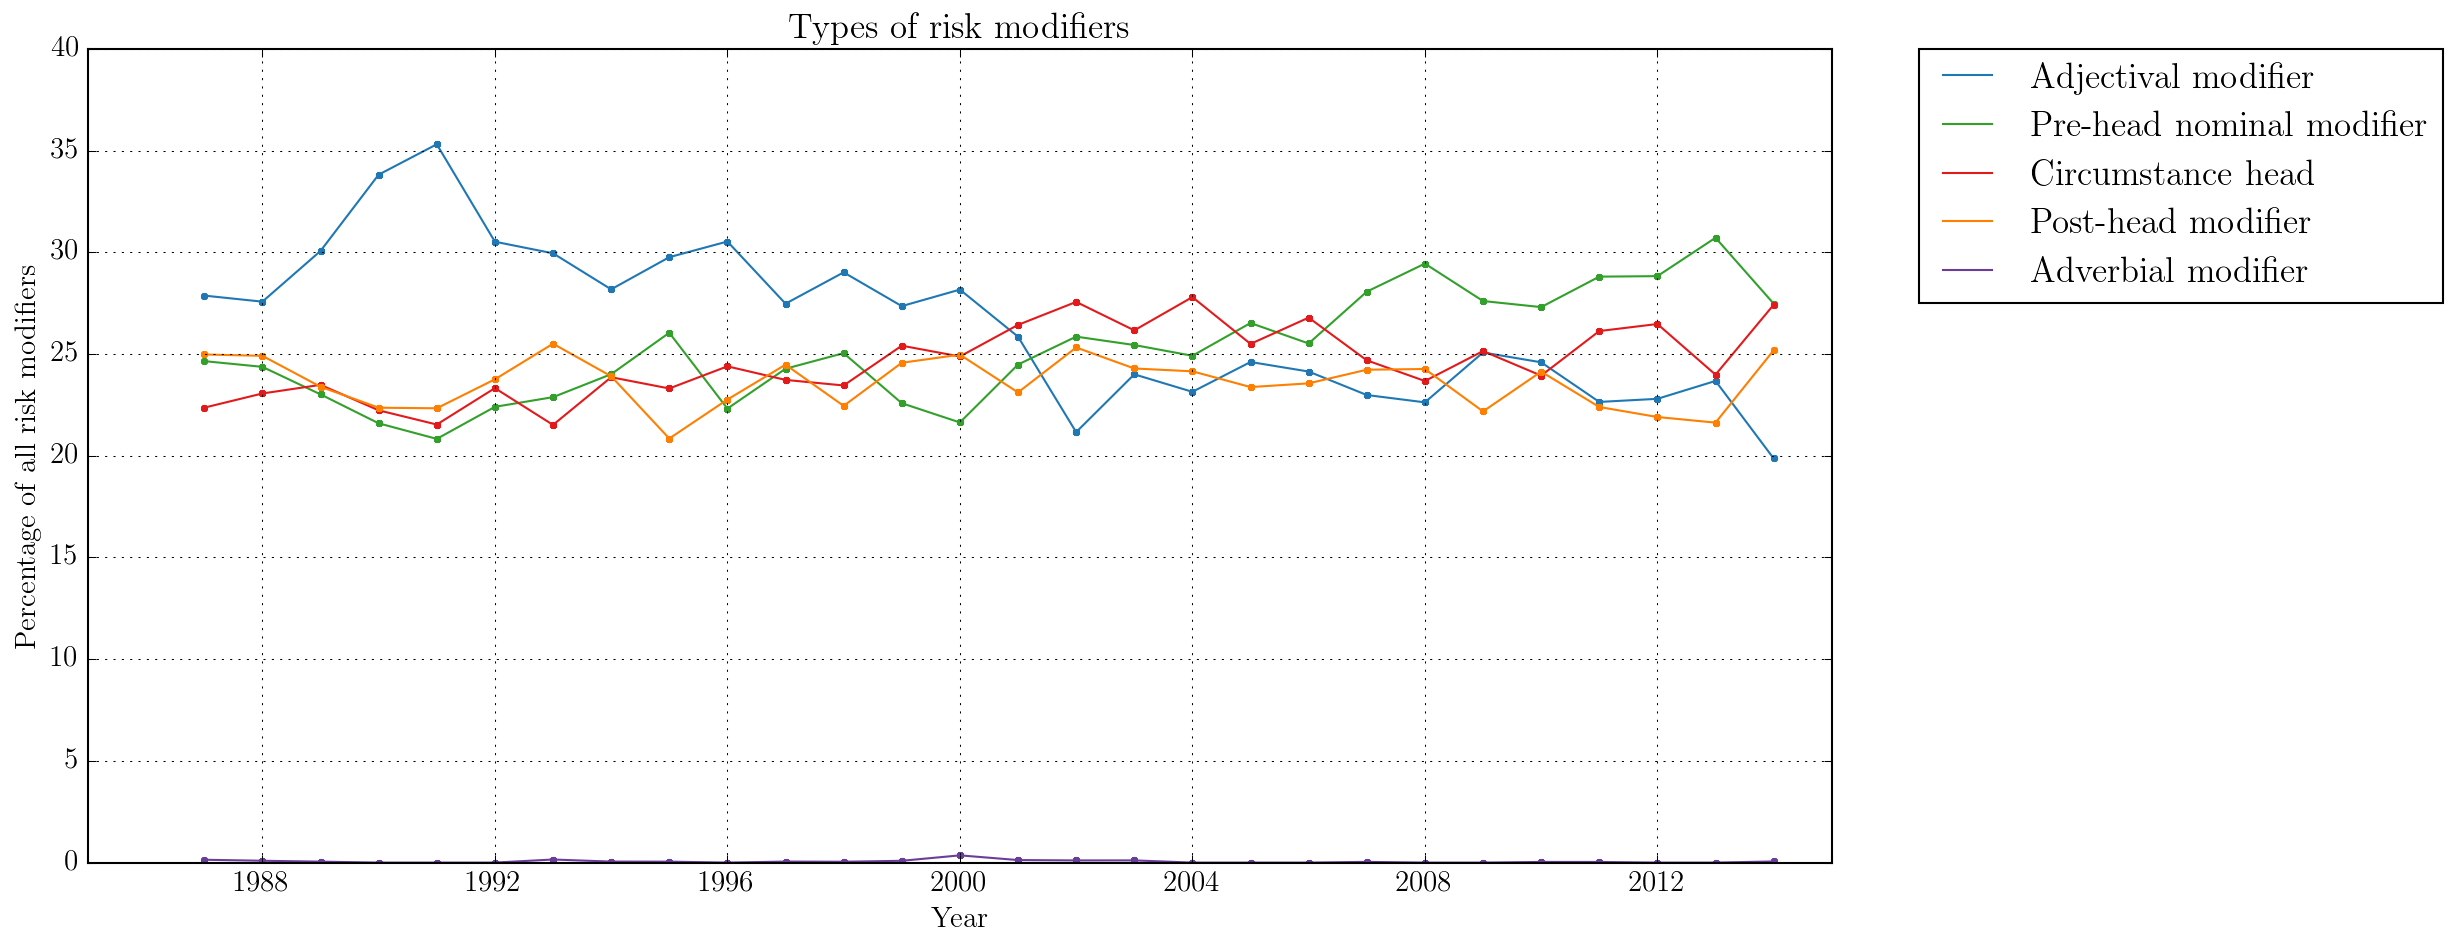
\includegraphics[width=0.98\textwidth]{../images/types-of-risk-modifiers.png}
    \captionof{figure}{Types of risk modifier}
    \label{fig:riskmod_types}
    \end{minipage}%
    \begin{minipage}{.433\textwidth}
    \centering
    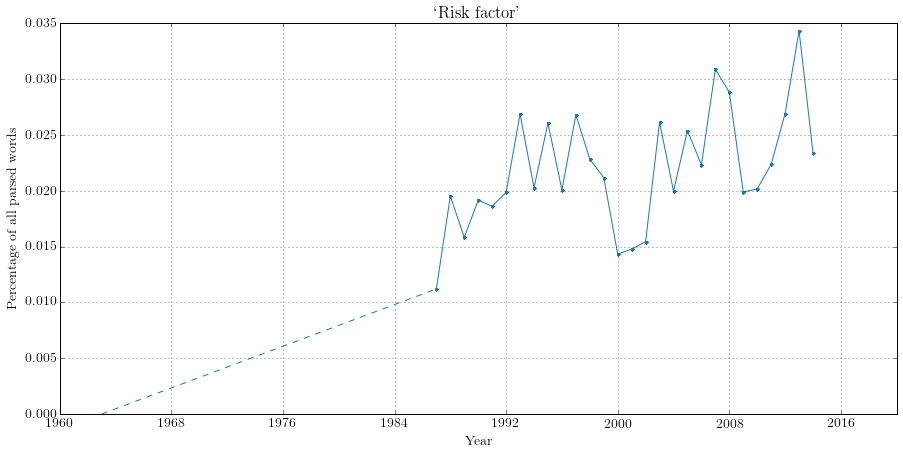
\includegraphics[width=0.98\textwidth]{../images/risk-factor.png}
    \captionof{figure}{Relative frequency of \emph{risk factor}}
    \label{fig:riskfactor}
    \end{minipage}
    \end{figure}


    Modifier risks are unique for their variety and diversity: through compounding, comprehensible new risk words and phrases can easily be created. The entire corpus contained 327 unique adjectival risk words, including \emph{non-risk}, \emph{de-risk}, \emph{once-risky}, \emph{take-no-risks}, \emph{risk-swapping}, \emph{risk-abhorrent}, \emph{price-for-risk}, \emph{post-risky}, \emph{pooled-risk}, \emph{personal-risk}, \emph{optimum-risk}, \emph{one-risk-factor}, \emph{one-pitch-can-end-his-career-risk} and \emph{low-risk-to-society}. That said, most of these occur no more than a handful of times. By far the most common were \emph{risky\slash riskier\slash riskiest} (15588 occurrences), \emph{high-risk} (5533), \emph{low-risk} (1086), \emph{at-risk} (902), \emph{risk-free} (883) and \emph{risk-taking} (789). Of these, four exhibited trajectory shifts (see Figure \ref{fig:adjtraj}). The basic adjectival forms (\emph{risky}, \emph{riskier}, \emph{riskiest}) are dominant in the 1963 sample, then decrease, and re-emerge in 2000. \emph{High-risk} though very rare (two instances) in 1963, has become more common, and stabilised in trajectory. \emph{Low-risk} and \emph{at-risk} are on a consistent inbound trajectory.

    \noindent
    \begin{figure}[htb!]
    \centering
    \begin{minipage}{.48\textwidth}
    \centering
    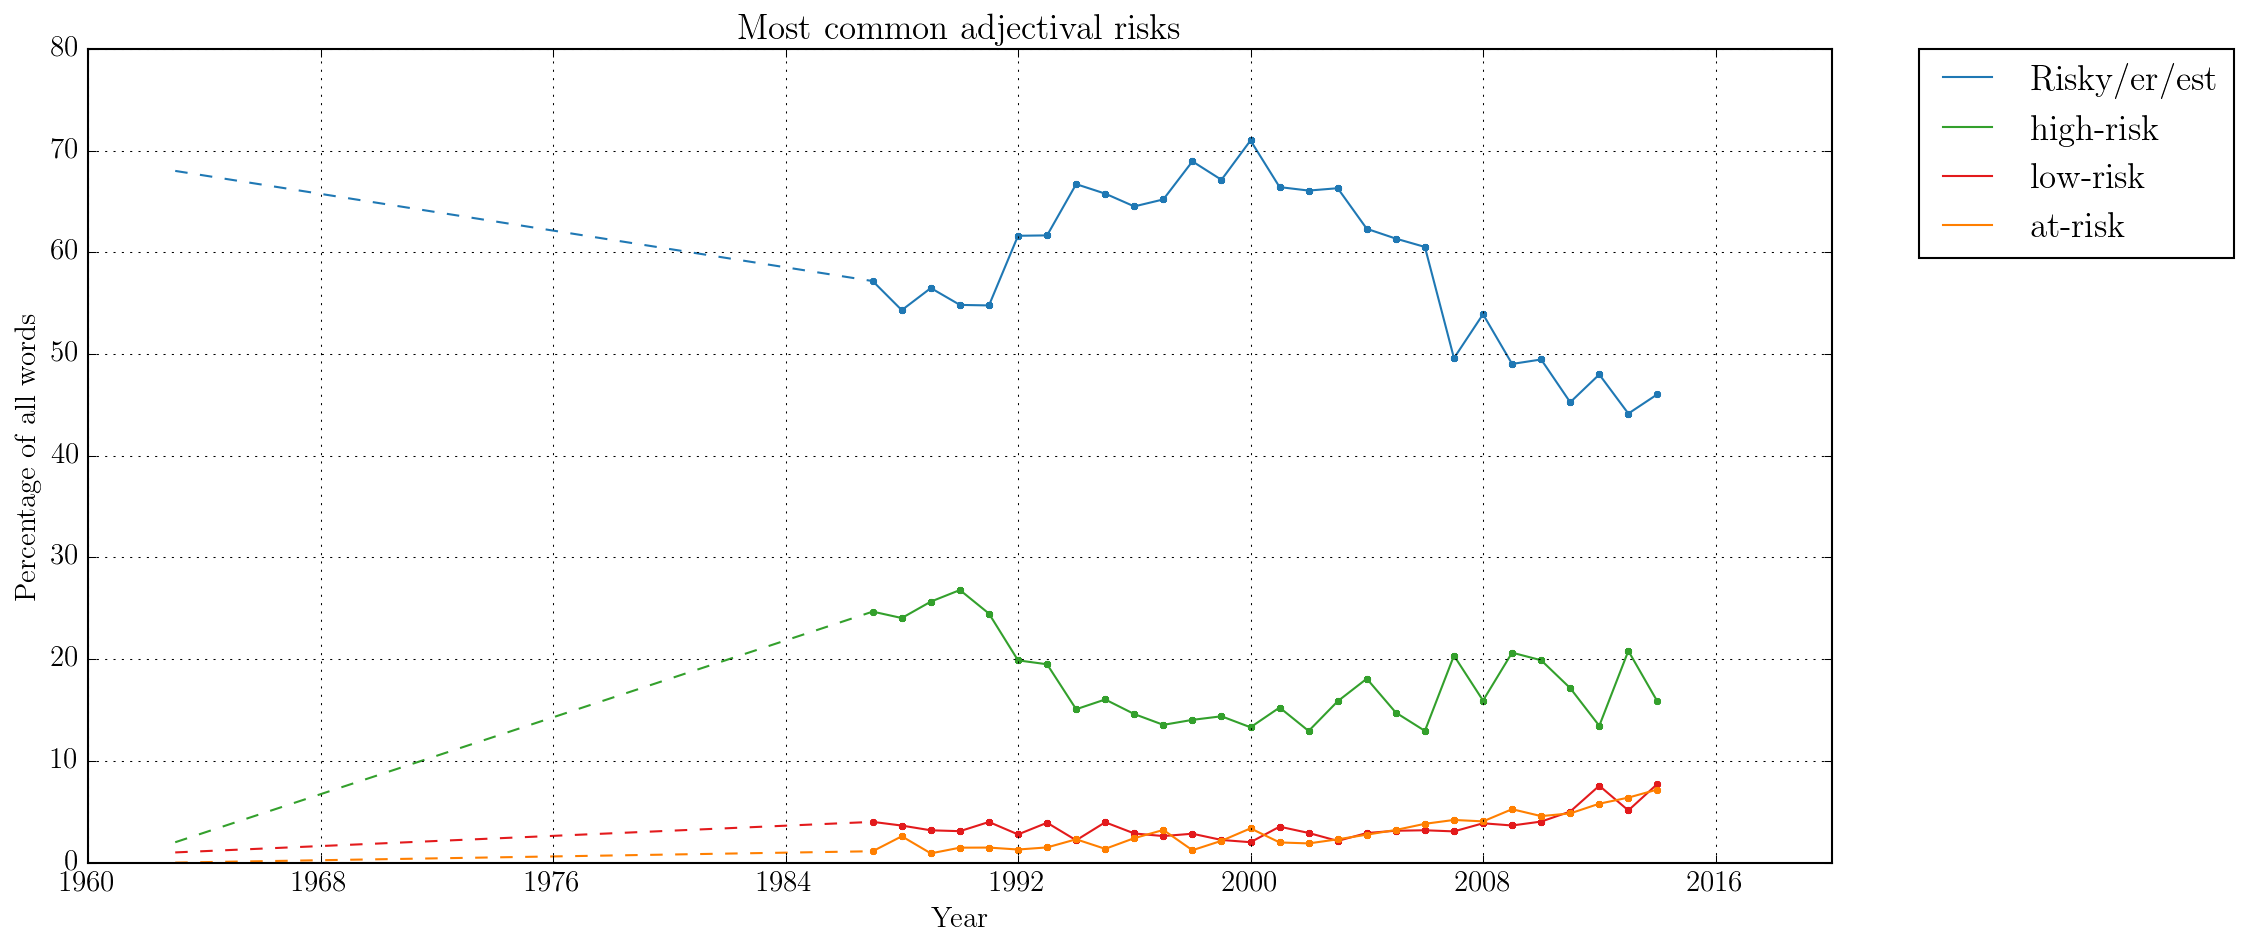
\includegraphics[width=0.98\textwidth]{../images/most_common_adjectival_risks.png}
    \end{minipage}%
    \begin{minipage}{.48\textwidth}
    \centering
    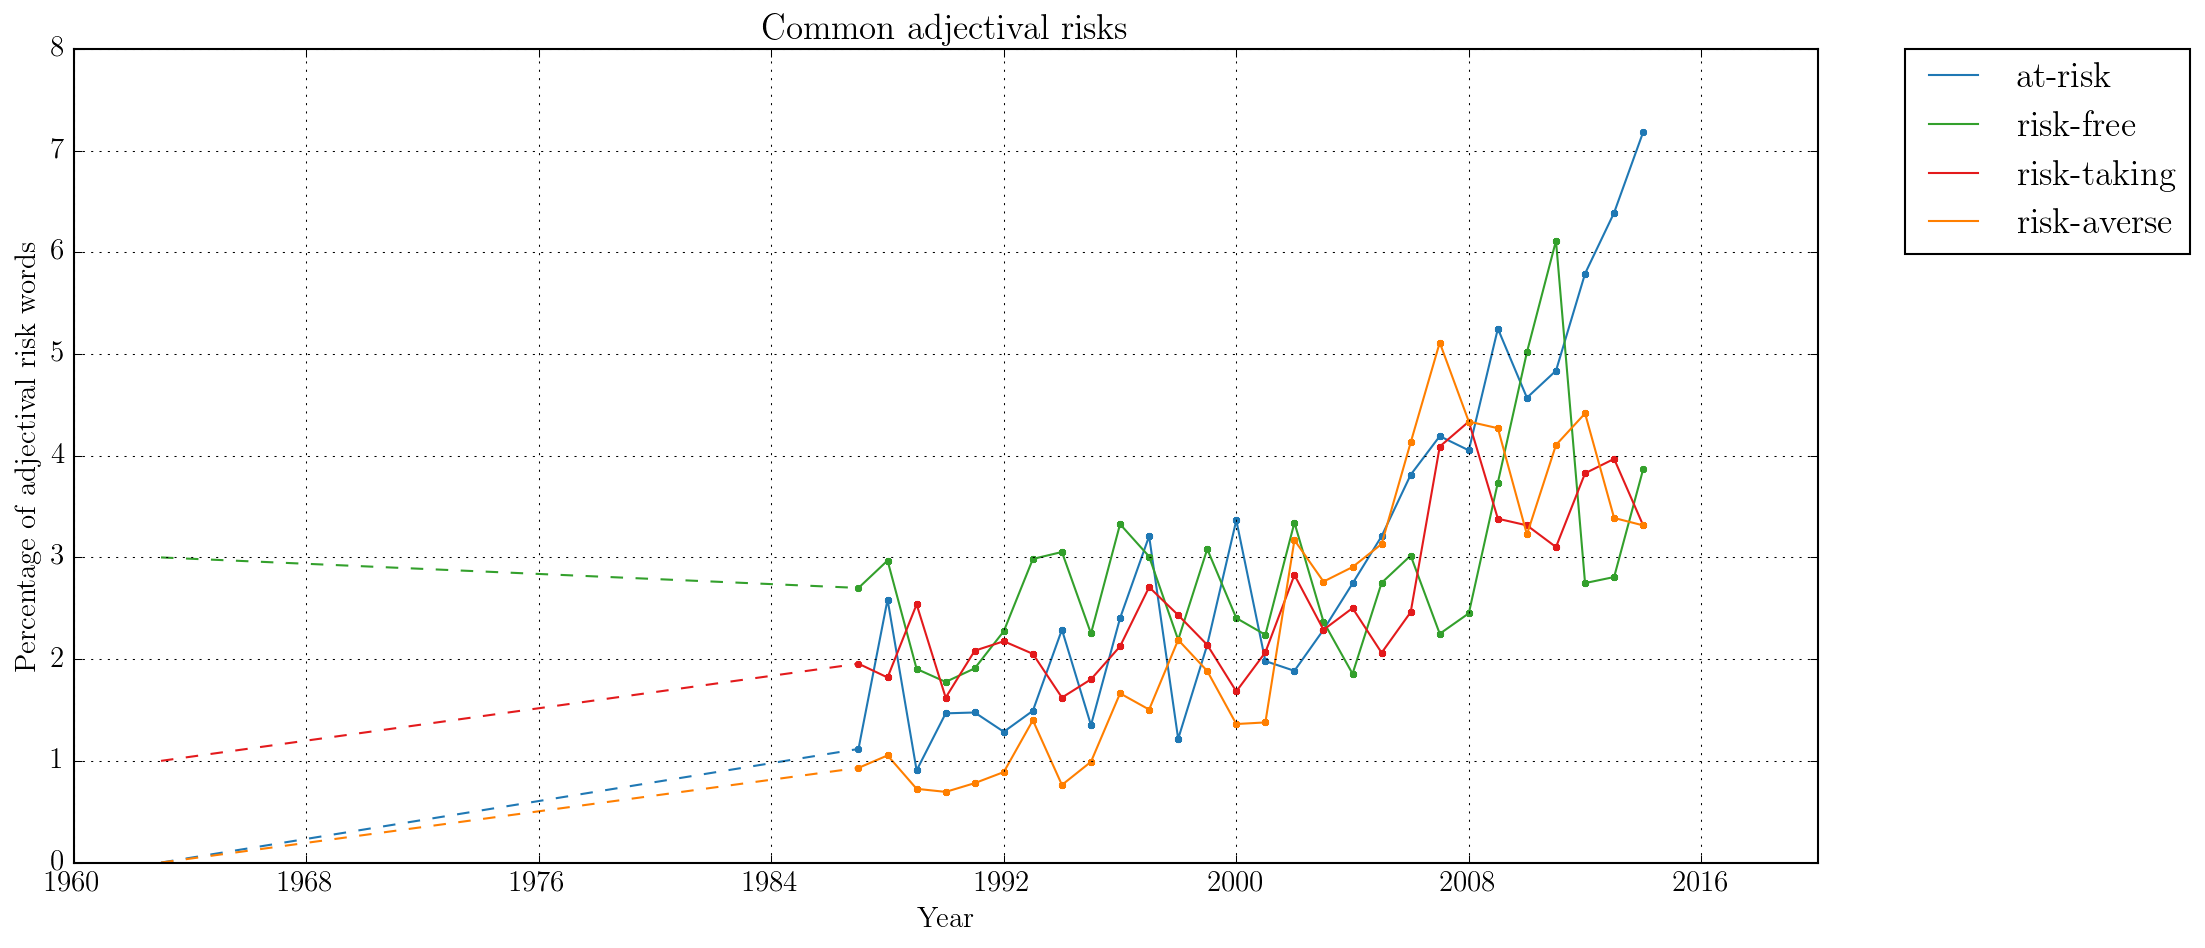
\includegraphics[width=0.98\textwidth]{../images/common_adjectival_risks.png}
    \end{minipage}
    \caption{Common adjectival risk words as percentage of all adjectival risks}
    \label{fig:adjtraj}
    \end{figure}

    The prevalence of high-risk in the 1980s is largely due to the AIDS epidemic: concordancing reveals that certain populations (gays, African Americans, Haitians) are at high-risk of being inflected by HIV. \emph{At-risk} is rare in earlier editions, but increases in prevalence steadily.

    This shift in risk is modifier is an important one. Low, moderate and high risk comprises a gradient, or scale, while at-risk is a binary. As with the shift toward \emph{potential risk}, this indicates both an increasing pervasiveness and a decreasing calcuability of risk. %remember that low-risk is actually increasing.
    
    %Of the graduated risks, low-risk is the only one on an inbound trajectory. What's the significance of this?



    %For people at moderate risk who also have two of the other risk factors , the treatment should be the same as for those in the high-risk group .
    %But ecologists , doctors and other specialists here warn that the entire population , not just high-risk groups , is vulnerable .
    %In the weeks since the law took effect , couples seeking marriage licenses have besieged hospitals , clinics and other doctors , anxious to get the test and the required counseling in time for wedding dates and quickly outnumbering those in high-risk groups most in need of attention .
    %Health experts say scarce funds for AIDS prevention would be better spent on high-risk groups .
    %Very few Americans know that Haitians have long since been removed from the list of high-risk groups because it was discovered that the H

    \vspace{5mm}\noindent\begin{tcolorbox}[colback=yellow!5,colframe=yellow!40!black,title=Summary: frequencies of modifier risk]
    \parbox{1\textwidth}{%
    Common risk modifiers (\emph{risky}, \emph{riskier}, \emph{riskiest}) are gradually being displaced by a number of less common constructions (e.g. \emph{low-risk}, \emph{at-risk}, \emph{risk-averse}, \emph{risk-free}).}
    \end{tcolorbox}
    \vspace{5mm}

\section{When risk is a modifier, what is being modified?} \FloatBarrier

    Risk as a modifier can be placed either before or after the noun it modifies (\emph{an at-risk person\slash a person at risk}). These two constructions are collapsed in Tables \ref{tab:riskmodified} and \ref{tab:atrisk}, which respectively list the participants most frequently modified by any risk modifier, and the participants most frequently modified by \emph{at-risk\slash at risk}. Note that while risk-modified participants generally are financial and economic in nature (\emph{investment, business, loan, asset}), the at-risk subset is mainly comprised of vulnerable populations of people (\emph{women}, \emph{children}, \emph{students}).

    \begin{table}[htb!]
    \centering
    \addvbuffer[12pt 8pt]{\begin{minipage}{.37\textwidth}
    \centering
    \small
    \begin{tabularx}{1.0\textwidth}{|X|l|}
    \hline
    \textbf{Risk-modified \mbox{participant}}        & \textbf{Total} \\ \hline
    investment  & 696   \\ \hline
    business    & 515   \\ \hline
    behavior    & 508   \\ \hline
    group       & 466   \\ \hline
    loan        & 421   \\ \hline
    asset       & 388   \\ \hline
    strategy    & 377   \\ \hline
    bond        & 346   \\ \hline
    area        & 307   \\ \hline
    venture     & 301   \\ \hline
    security    & 287   \\ \hline
    patient     & 265   \\ \hline
    pool        & 239   \\ \hline
    bet         & 214   \\ \hline
    move        & 204   \\ \hline
    activity    & 201   \\ \hline
    proposition & 199   \\ \hline
    child       & 170   \\ \hline
    woman       & 161   \\ \hline
    student     & 158   \\ \hline
    \end{tabularx}
    \caption{Most common risk-modified participants in the corpus}
    \label{tab:riskmodified}
    \end{minipage}} \hspace{1cm}
    \addvbuffer[12pt 8pt]{\begin{minipage}{.37\textwidth}
    \small
    \begin{tabularx}{1.0\textwidth}{|X|l|}
    \hline
    \textbf{At-risk \mbox{participant}}       & \textbf{Total} \\ \hline
    person     & 439   \\ \hline
    child      & 368   \\ \hline
    woman      & 209   \\ \hline
    student    & 179   \\ \hline
    nation     & 135   \\ \hline
    patient    & 110   \\ \hline
    youngster  & 93    \\ \hline
    group      & 91    \\ \hline
    population & 64    \\ \hline
    family     & 58    \\ \hline
    kid        & 50    \\ \hline
    youth      & 48    \\ \hline
    money      & 48    \\ \hline
    worker     & 45    \\ \hline
    life       & 41    \\ \hline
    job        & 41    \\ \hline
    man        & 40    \\ \hline
    area       & 35    \\ \hline
    teenager   & 32    \\ \hline
    other & 32 \\ \hline
    \end{tabularx}
    \caption{Most common at-risk participants in the corpus}
    \label{tab:atrisk}
    \end{minipage}}% This must go next to `\end{minipage}`
    \end{table}

    In need of further research is whether or not the list of entities that can sensibly be modified by \emph{at-risk} is beginning to grow: since the U.S. subprime mortgage crisis (beginning in 2007), references to \emph{at-risk homeowners} appear to be on the rise. Results from 2011, for example, show that \emph{nations} and even \emph{economic sectors} are being modified with \emph{at-risk}:

    \begin{enumerate}  [before=\itshape,font=\normalfont] \setlength\itemsep{0em} \small
    \item Mr. Obama asked for \$400 million for the World Bank's clean technology fund, \$95 million for the bank's program to prevent deforestation and \$90 million for its program to help at-risk nations cope with the effects of a warming planet by, for instance, developing drought-resistant crops.
    \item The most at-risk sectors included auto components and automobile companies, which generate nearly 30 percent of their sales in Europe, as well as food and tobacco firms.
    \end{enumerate}

    Note that it is difficult to reconcile the semantic meaning of \emph{at-risk} constructions with the semantic frame of risk provided by \citeA{fillmore_toward_1992}. Though elements of both the \textsc{victim} and \emph{valued object} appear to be at work, neither provides an adequate label for \emph{at-risk people, children, homeowners or nations}. Rather than being an oversight during the articulation of the risk frame (recall Figure~\ref{fig:fil_atk}), in light of the increased use of these kinds of constructions since the mid 1990s, we hypothesise that \emph{at-risk} constructions (as well as \emph{to put at risk}) are demonstrative of a broader shift in risk discourse toward general clusters of negative outcomes, rather than specific and measurable potential harms. Connection between this shift and sociological theory is made in the following chapter.

    \vspace{5mm}\noindent\begin{tcolorbox}[colback=yellow!5,colframe=yellow!40!black,title=Summary: participants modified by risk]
    \parbox{1\textwidth}{%
    While risk as a modifier is often used in the context of finance\slash commerce, \emph{at-risk} typically attaches to vulnerable human demographics.}
    \end{tcolorbox}
    \vspace{5mm}

\section{How arguable is risk?} \label{sect:arguability} \FloatBarrier

    As noted earlier, our central concern with the Mood system is the degree of arguability associated with the concept of risk. Risk in Subject, Finite and Predicator positions is the most arguable. Risk words within Complements and Adjuncts are less arguable.

    %A dependency grammar attempts to locate a lexical root for each clause, and attach dependents to it recursively until no lexical items are unattached. Each word is ordered by its dependency to the root of a clause. The nature of the dependency relationship can also be provided. Such grammars are particularly useful for free word order language, but have been applied to English successfully as well.

    Based on the kinds of parsing provided by Stanford CoreNLP, it was possible to measure arguability in two ways. First, we can map dependency relationships to the systemic-functional notion of arguability. A dependency grammar locates the predicator of a clause and assigns it a position of zero. A `1' is then assigned to its most immediate dependent (other components in the verbal group, if present, or the head of the Subject, if not). This process continues until no lexical items are unattached, or `ungoverned'. In effect, the higher the number attached to a word, the further it is semantically from being an important component in the meaning, and thus, in systemic functional terms, the less arguable the word.

    \begin{figure}[htb!]
    \centering
    \addvbuffer[12pt 8pt]{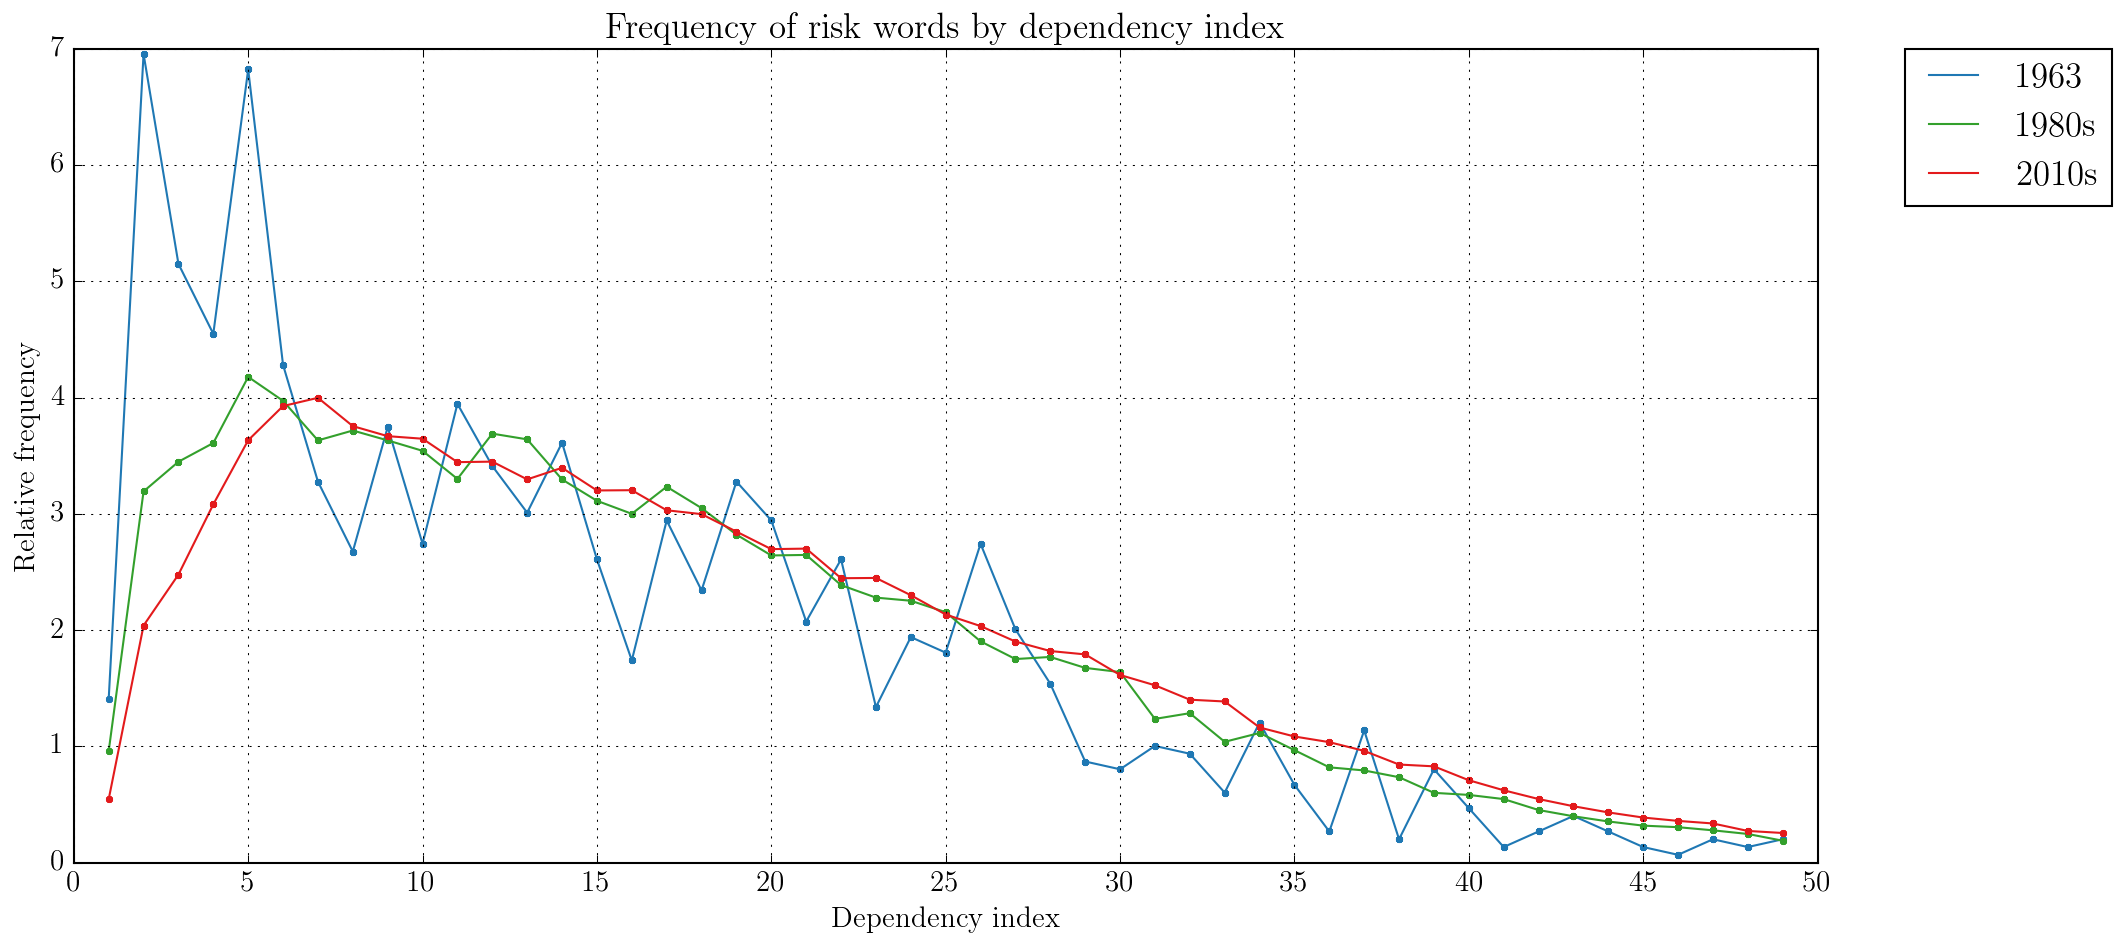
\includegraphics[width=0.75\textwidth]{../images/frequency-of-risk-words-by-dependency-index.png}}
    \caption{Risk words by dependency position in clause}
    \label{fig:depnum}
    \end{figure}
    %
    Highlighting three sampling periods as in Figure \ref{fig:depnum} shows that in early samples, risk occupies core roles within the dependency hierarchy, and thus sits closer to the core part of the meaning being exchanged within the clause. In later samples, risk more commonly occurs later in the dependency structure, in less focial positions. As explained earlier, though this experimental method is not a perfectly reliable indicators of arguability, it does indicate an increasing preference to position risk as non-core, ancillary information, rather than as the main thing which is under discussion.

    %\endnote{Dependency place 2 and 3 removed from visualisation, as these roles are typically for finites and modal auxiliaries---positions that a risk word cannot grammatically fill.}

    The second thing we can use dependency output for is identifying the functional roles of risk words. This is more accurate than using the dependency ranking, but creates a long list of functional roles. Of key interest, however, are risk words at the head of each major component of the Mood system---Subject, Finite\slash Predicator, Complement and Adjunct (CoreNLP parses unfortunately do not distinguish between Finite and Predicator in a reliable way, so the categories are collapsed here). From Figure \ref{fig:interpersonalarg}, we can see that risk is shifting from Subject and Finite\slash Predicator to Complement and Adjunct roles. This is an important result: risk words in more arguable roles are steadily decreasing, while risk in less arguable roles are becoming more common. Like earlier findings, this suggests an increasing implicitness of risk in NYT discourse, with less talk actually \emph{about} risk, but more talk where the relationship between risk and the subjects of the talk is assumed to be more or less common knowledge.

    \noindent
    \begin{figure}[htb!]
    \centering
    \begin{minipage}{.48\textwidth}
    \centering
    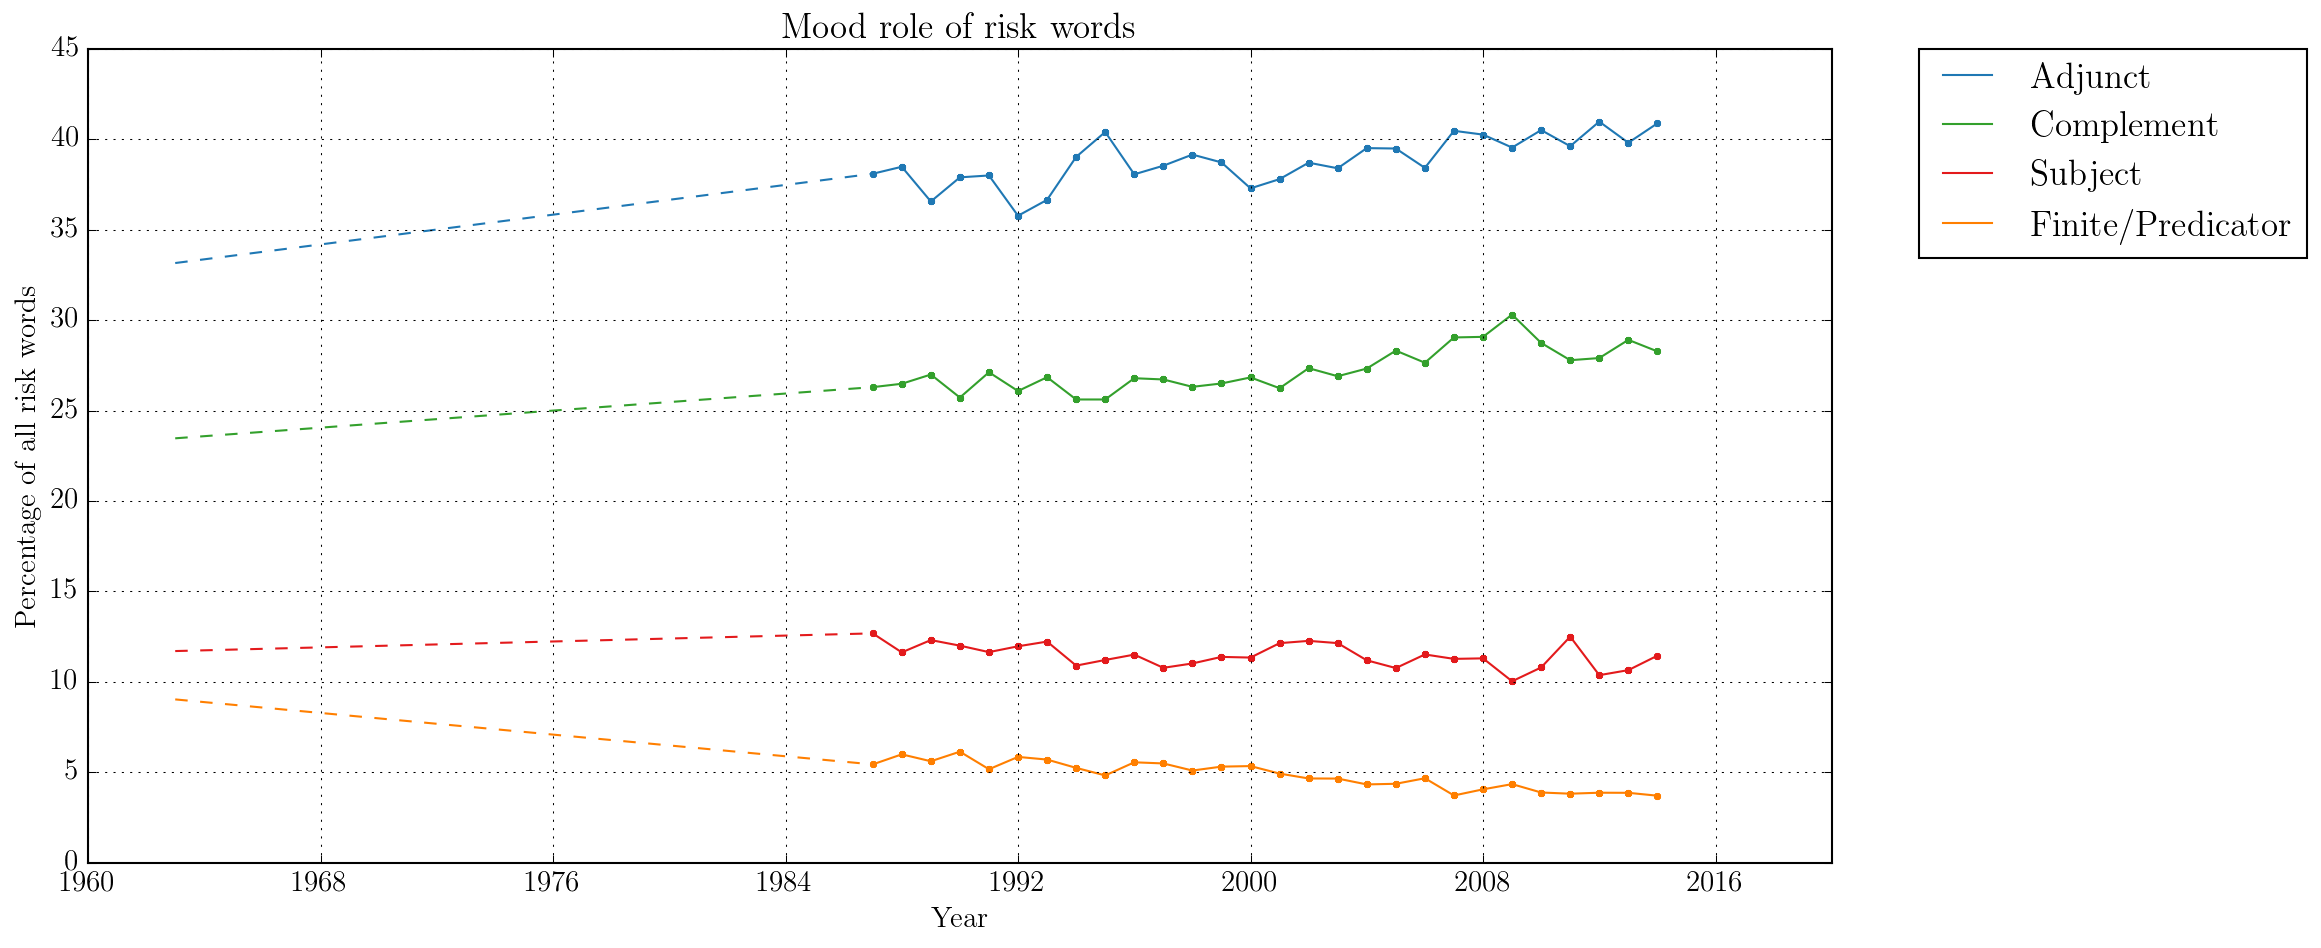
\includegraphics[width=0.98\textwidth]{../images/mood_role_of_risk_words.png}
    \end{minipage}%
    \begin{minipage}{.48\textwidth}
    \centering
    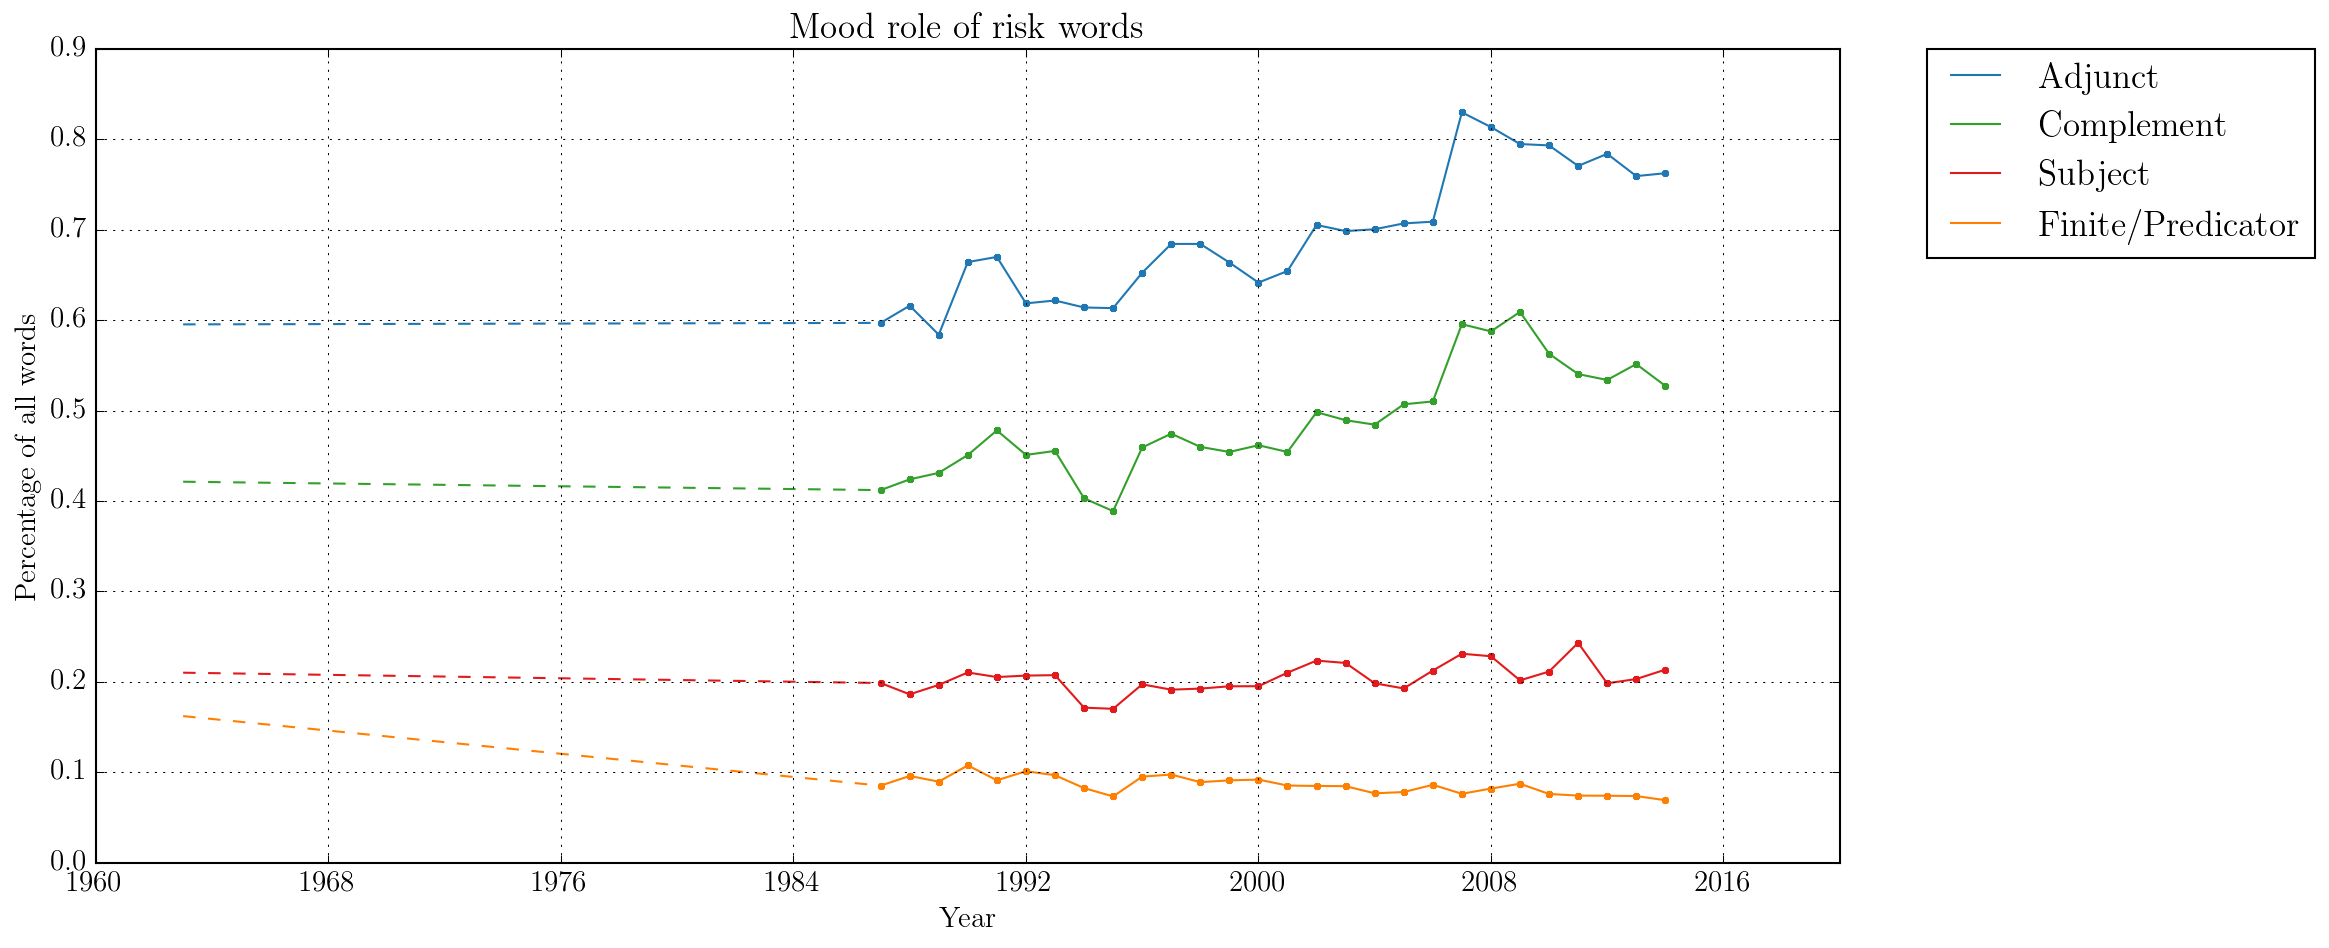
\includegraphics[width=0.98\textwidth]{../images/riskdep_allwords.png}
    \end{minipage}
    \caption{Frequency of risk words for each Mood component as percentage of all risk words\slash all parsed data}
    \label{fig:interpersonalarg}
    \end{figure}

    %By providing each role with a relative weight, we can plot arguability as a single decreasing trend line, showing the increased implicitness of risk within the language of the NYT.

    %Using the full list of risk dependencies, we can also locate more specific constructions undergoing trajectory shift. Figure \ref{fig:salienttrajectories} shows that risk is increasingly instantiated within prepositional phrases (which are by their nature dependent on Participants and Processes), and decreasingly as a predicator. From this view too, risk words are increasingly implicit within news language.

    \vspace{5mm}\noindent\begin{tcolorbox}[colback=yellow!5,colframe=yellow!40!black,title=Summary: risk and arguability]
    \parbox{1\textwidth}{%
    Longitudinally, risk words are shifting to less focal parts of clauses. We can approximate these changes using both indices or semantic function information within dependency parses.}
    \end{tcolorbox}
    \vspace{5mm}

\section{Risk words and proper nouns} \FloatBarrier

    We searched for proper noun groups in parse trees containing a risk word. This is a departure from many of our earlier queries, as here we are looking only at which entities co-occur with risk language, rather than determining how risk words and non-risk words relate to other another lexicogrammatically. The result of this query was 68891 different proper noun groups. We took the 200 most common results, and merged any that denoted the same entity: \emph{F.D.A.\slash Food and Drug Administration}, or \emph{Federal Reserve and Fed}. We then grouped results into thematic categories: \emph{People}, \emph{Nations}, \emph{Geopolitical entities}, \emph{Companies}, \emph{Organisations} and \emph{Medical themes}. The results were then plotted (See Figure \ref{fig:propernouns}). 

    \begin{landscape}
    \centering
    \begin{figure}
    \captionsetup[subfigure]{oneside,margin={-1.5cm,-.5cm}}
    \centering % [t!] % "[t!]" placement specifier just for this example
    \begin{subfigure}{.64\textwidth}
    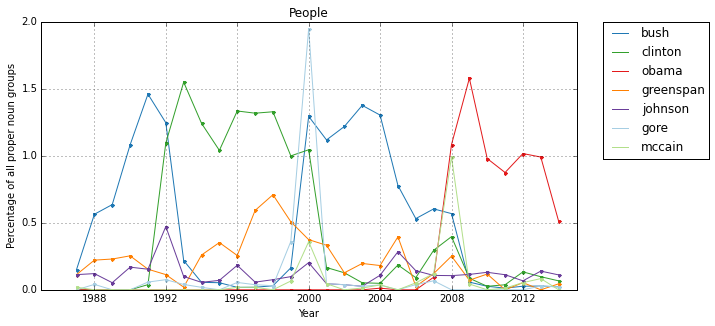
\includegraphics[width=\linewidth]{../images/people}
    \caption{People} \label{fig:a}
    \end{subfigure}
    \begin{subfigure}{.64\textwidth}
    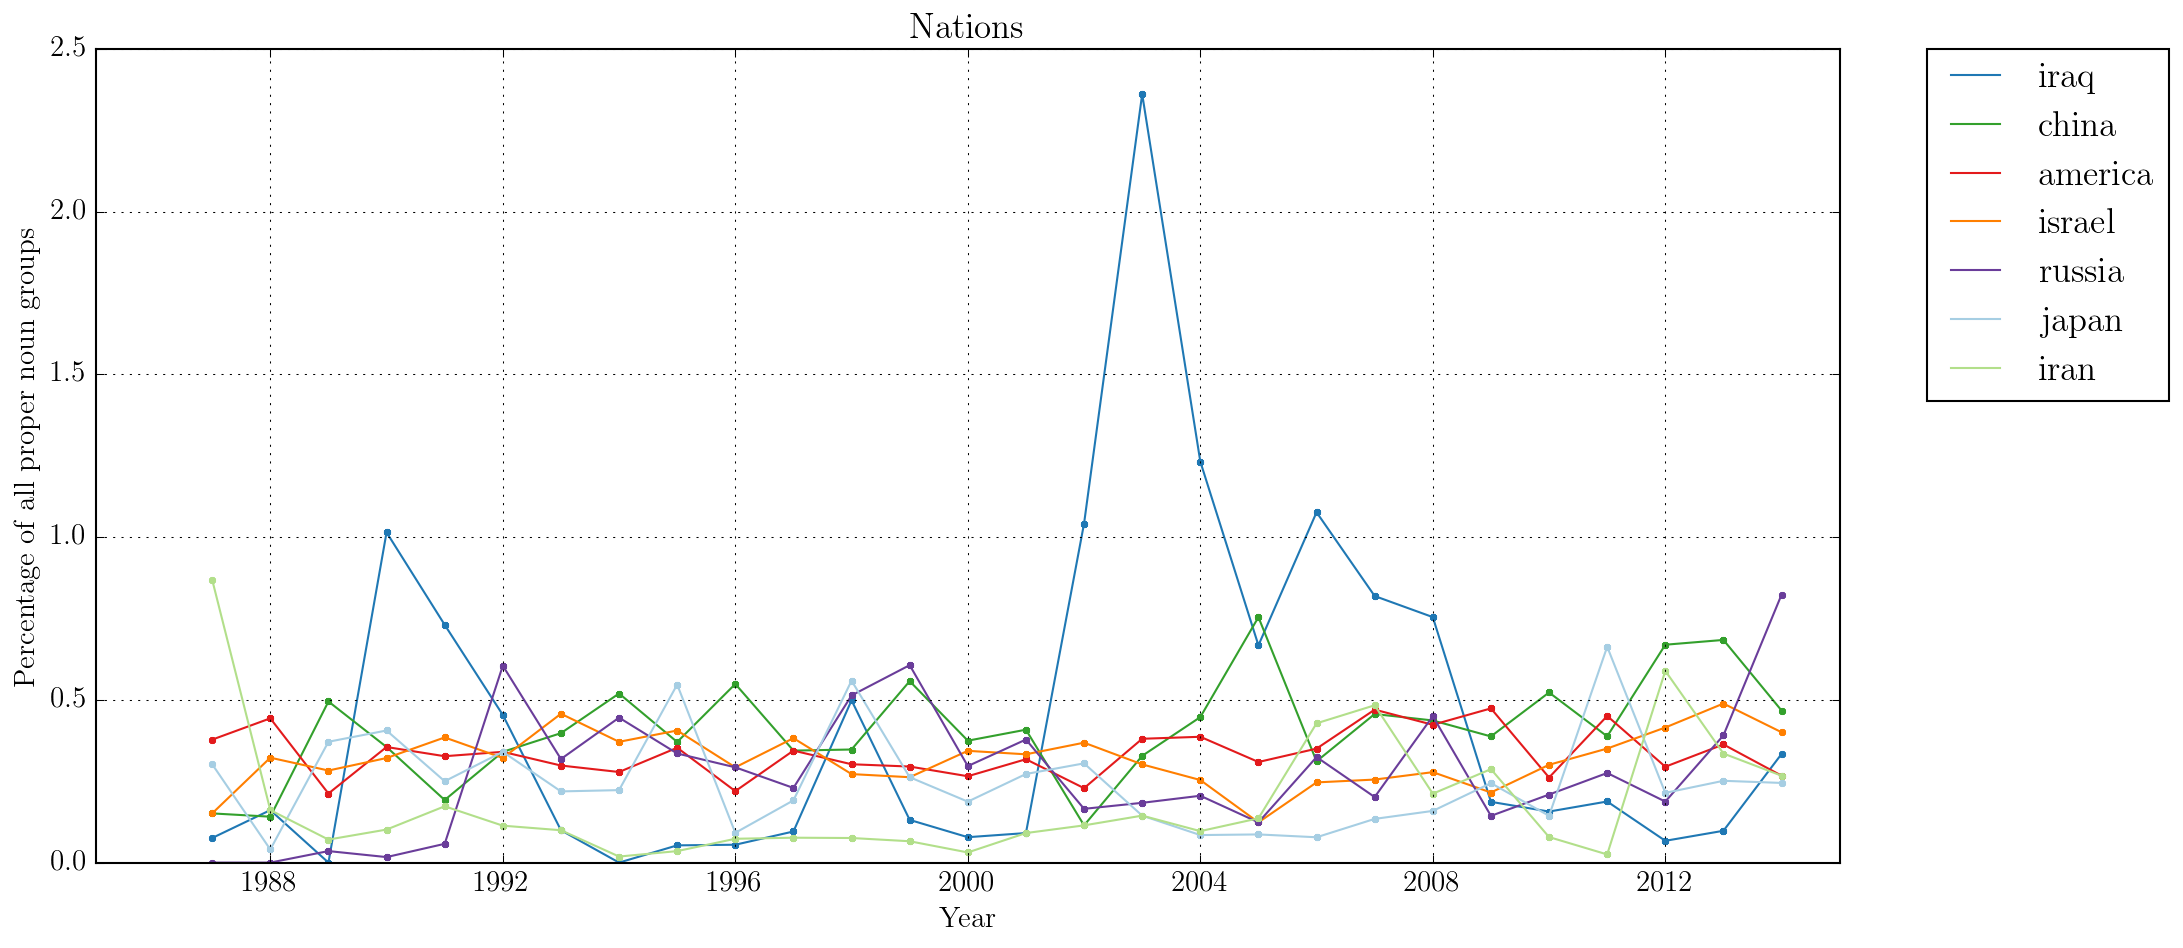
\includegraphics[width=\linewidth]{../images/nations}
    \caption{Nations} \label{fig:b}
    \end{subfigure}

    \medskip
    \begin{subfigure}{.64\textwidth}
    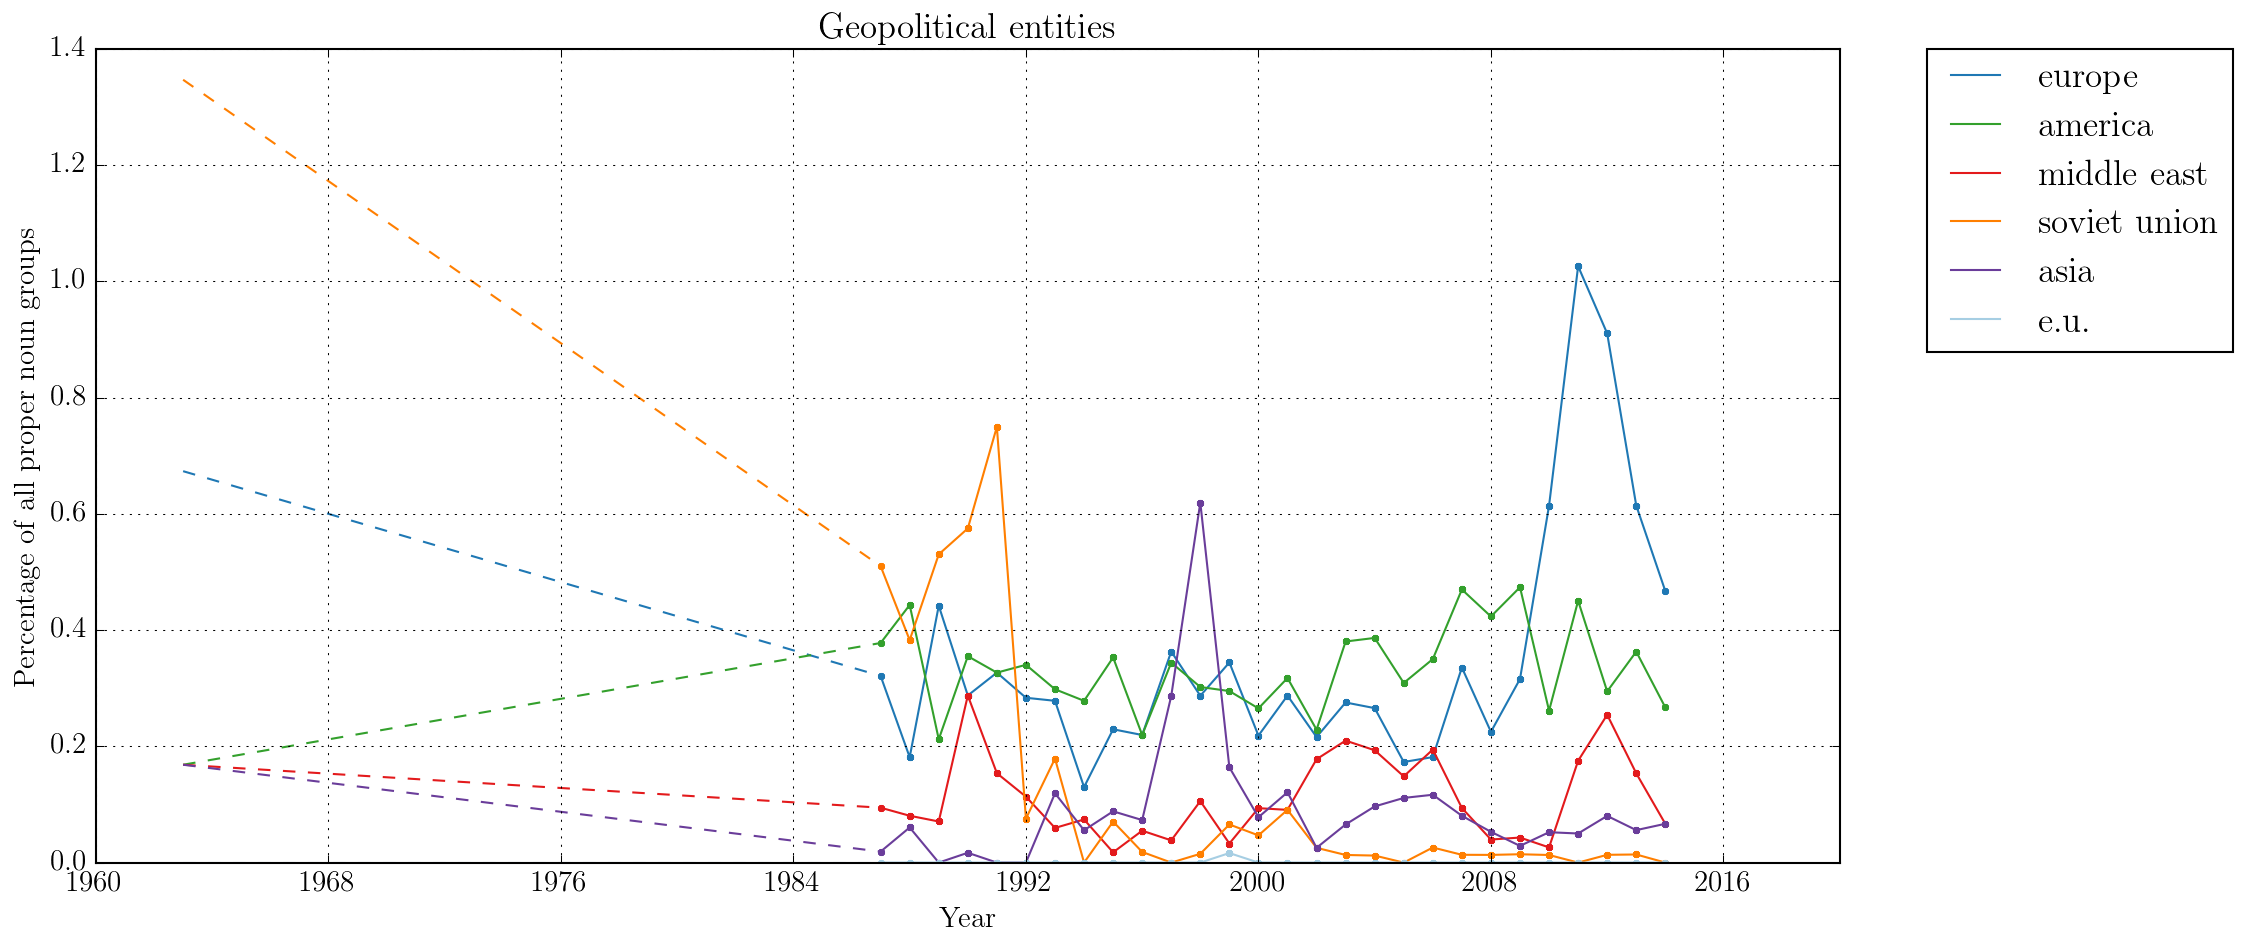
\includegraphics[width=\linewidth]{../images/geopolitical_entities}
    \caption{Geopolitical entities} \label{fig:c}
    \end{subfigure}
    \begin{subfigure}{.64\textwidth}
    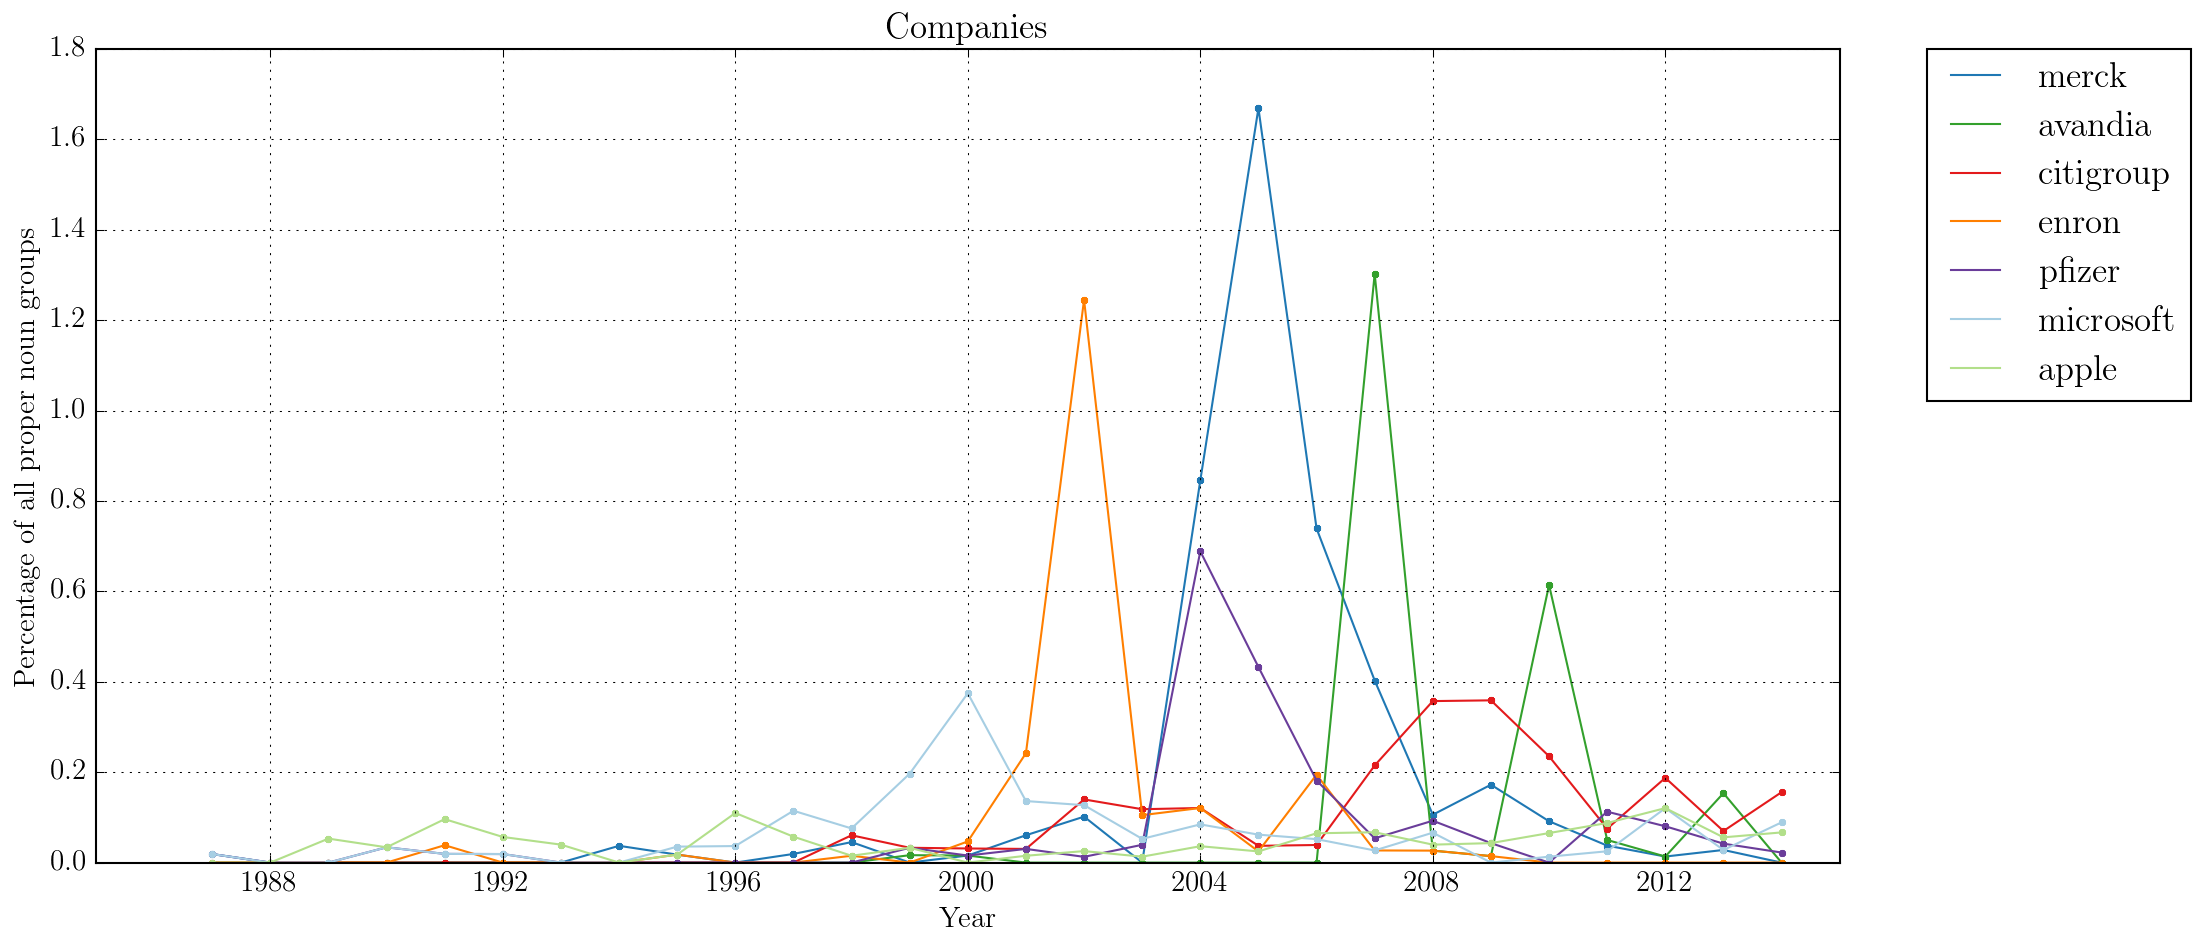
\includegraphics[width=\linewidth]{../images/companies}
    \caption{Companies} \label{fig:d}
    \end{subfigure}

    \medskip
    \begin{subfigure}{.64\textwidth}
    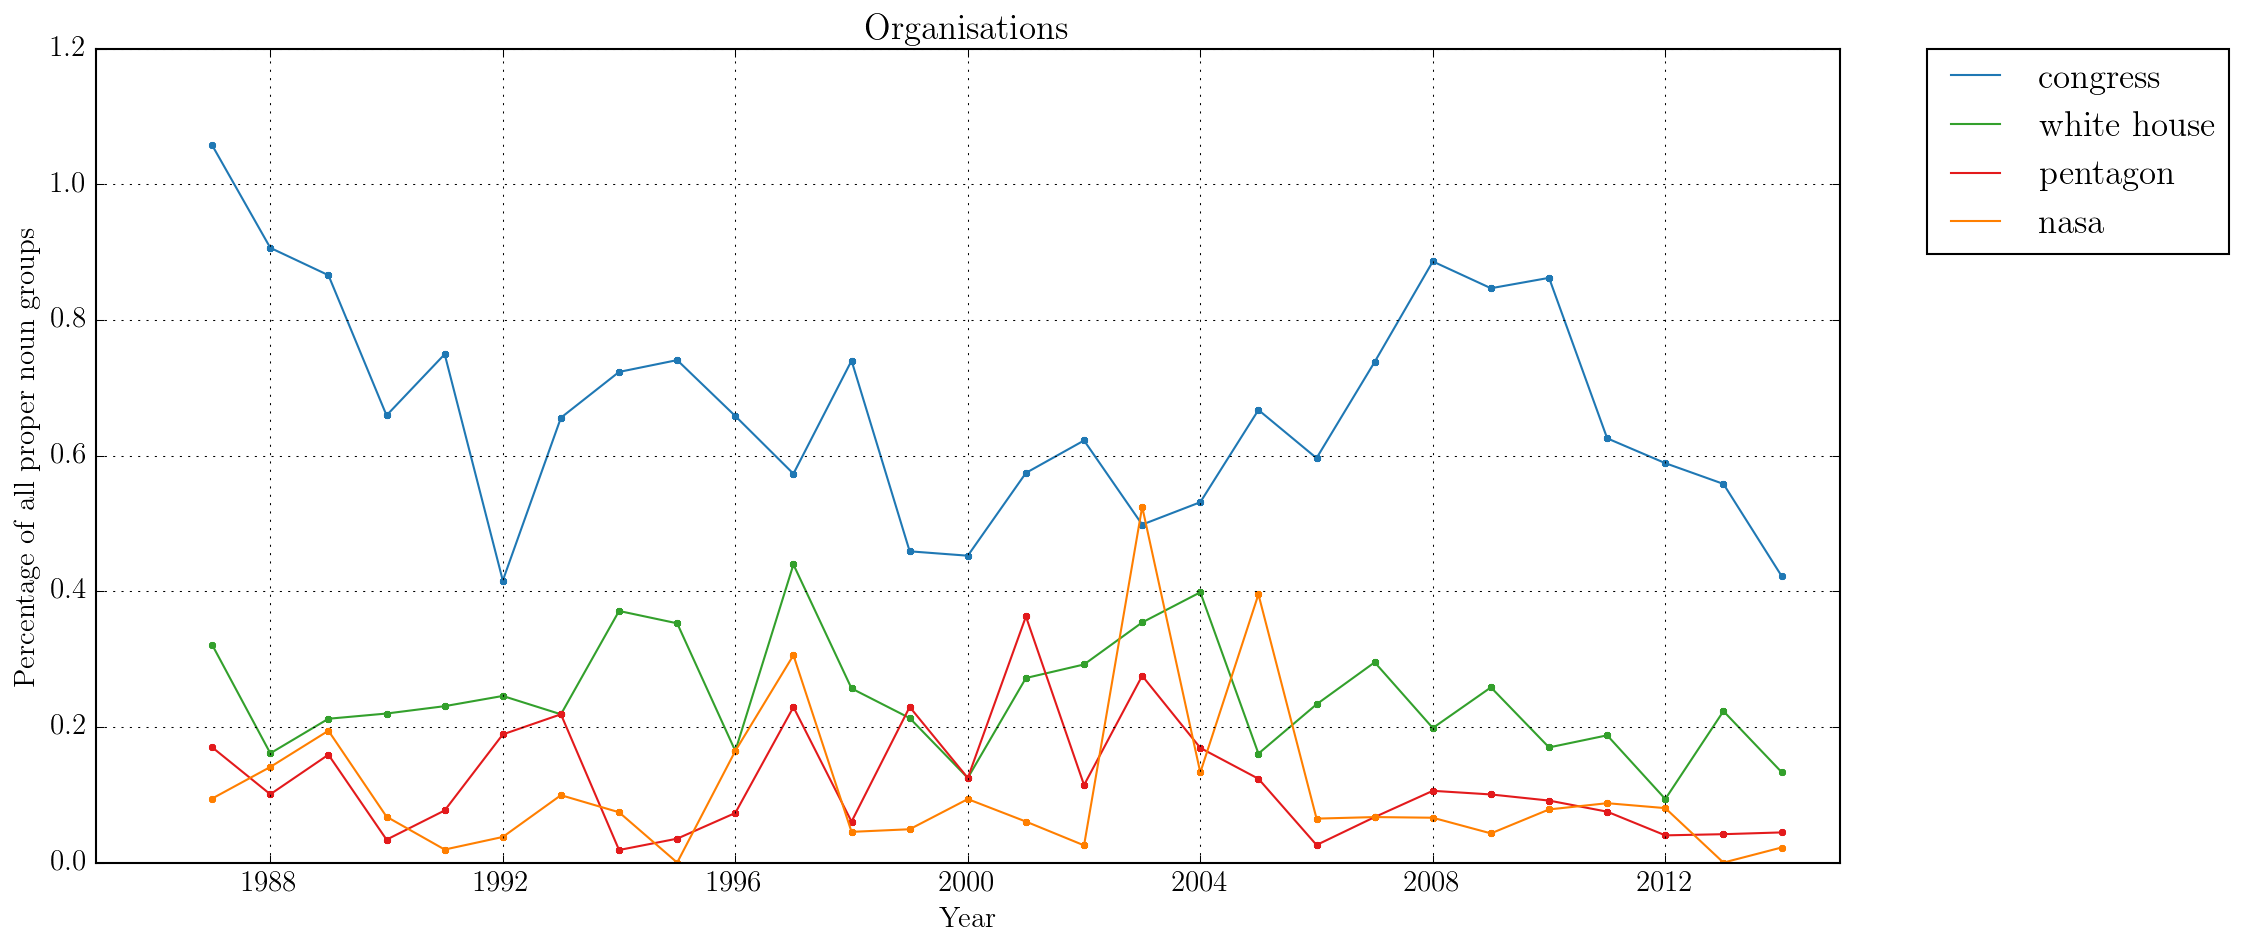
\includegraphics[width=\linewidth]{../images/organisations}
    \caption{Organisations} \label{fig:e}
    \end{subfigure}
    \begin{subfigure}{.64\textwidth}
    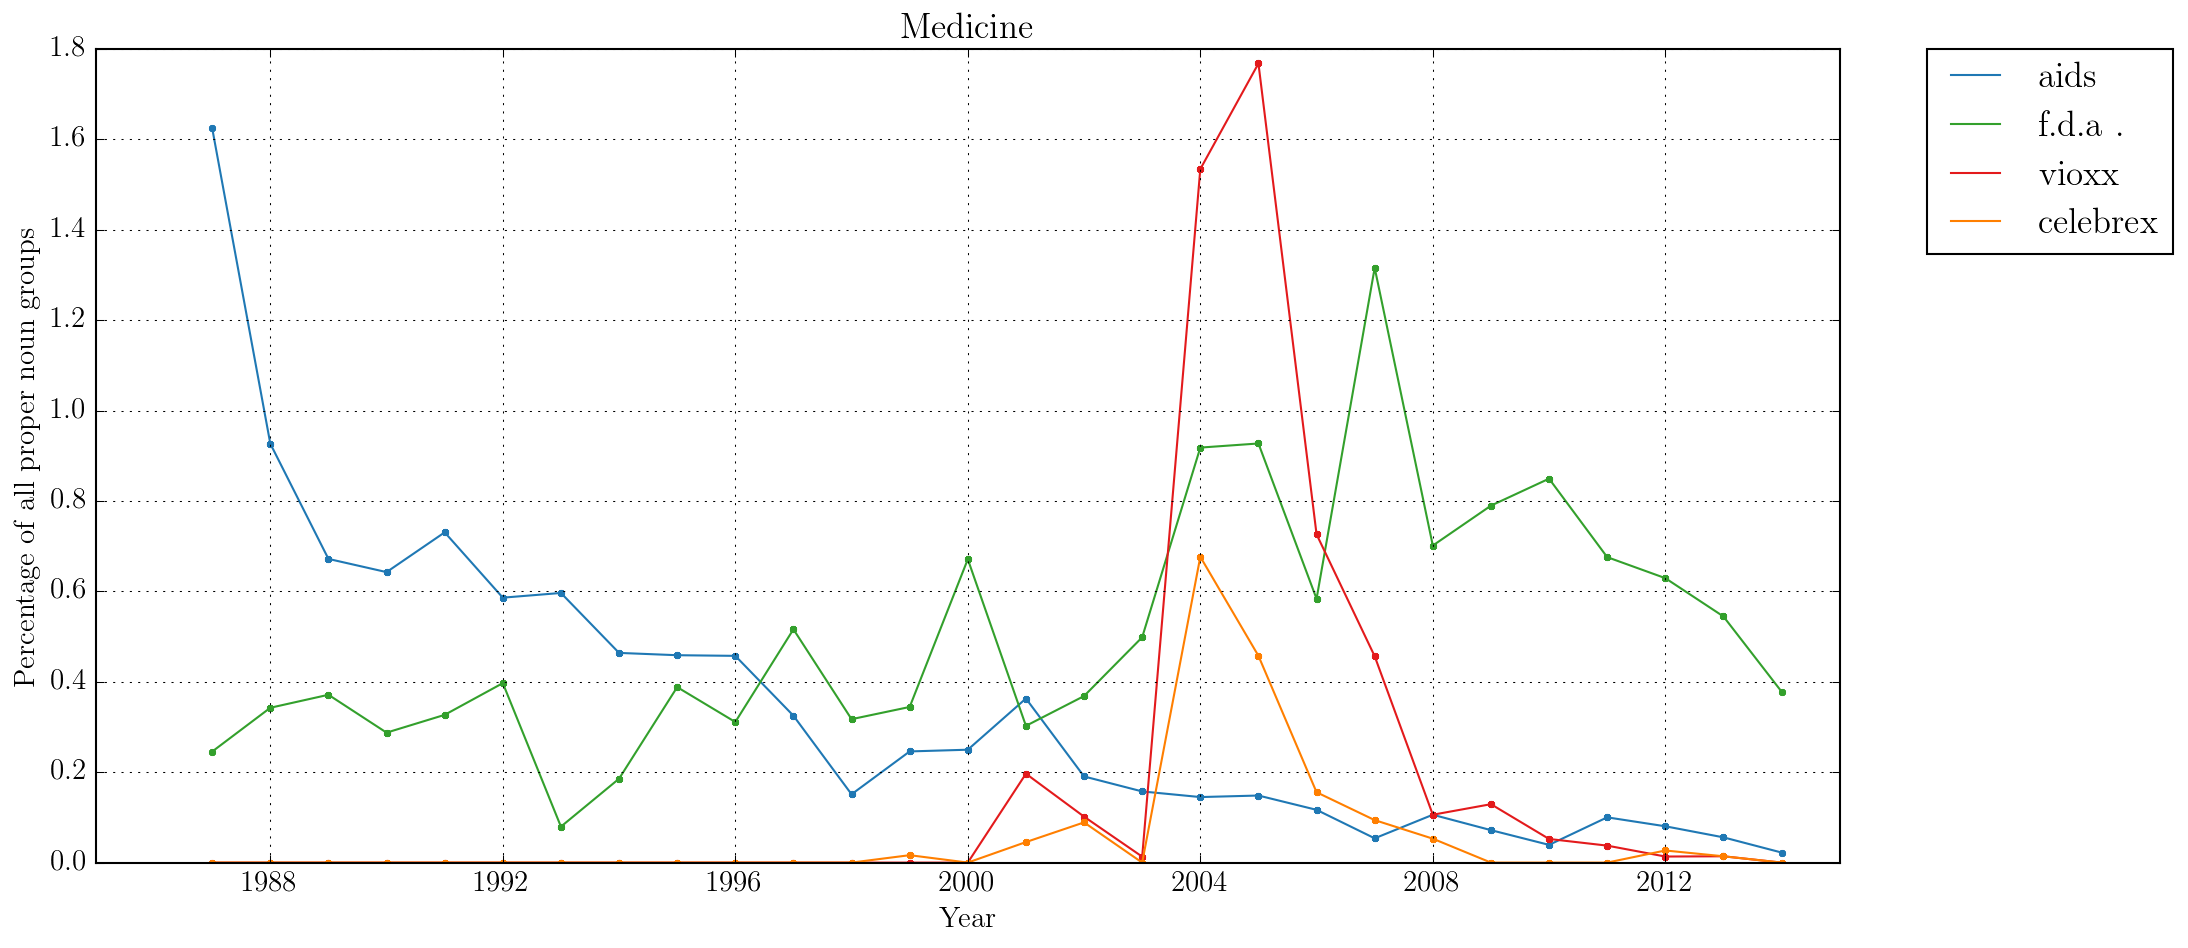
\includegraphics[width=\linewidth]{../images/medicine}
    \caption{Medical terms} \label{fig:f}
    \end{subfigure}
    \caption{Proper noun groups co-occurring with risk} \label{fig:propernouns}
    \end{figure}
    \end{landscape}

    A number of historical events were easily recognisable within the peaks and troughs of these charts. Key events represented through these interrogations include:

    \begin{enumerate} \setlength\itemsep{0em}
    \item US presidents and presidential candidates\endnote{Though the filtering out of titles and given names collapses the distinction between Bushes and Clintons, we can still reasonably infer which was being spoken about at which, and doubt can be eliminated by concordancing}~(Figure~\ref{fig:a})
    \item The First Persian Gulf War (Figure~\ref{fig:b})                   
    \item The Iraq Wars (Figure~\ref{fig:b})
    \item September 11 and the War in Afghanistan (Figure~\ref{fig:b})   
    \item The beginning of the 2014 Crimean crisis (Figure~\ref{fig:b})       
    \item The Asian financial crisis (Figure~\ref{fig:c})
    \item The breakup of the Soviet Union (Figure~\ref{fig:c})
    \item The Eurozone crisis (Figure~\ref{fig:c})
    \item The Space Shuttle Colombia Disaster (Figure~\ref{fig:d})
    \item The collapse of Enron (Figure~\ref{fig:e})
    \item The U.S. subprime mortgage crisis  (Figure~\ref{fig:e})
    \item The U.S. outbreak of HIV and the AIDS crisis (Figure~\ref{fig:f})
    \item The recall of Vioxx (Figure~\ref{fig:f})
    \end{enumerate}
    %
    This area of our investigation is by far the most promising as a means of connecting risk language to particular people and events. Spatial considerations have precluded a full treatment of the charting of risk language to specific events, despite the fact that enough data exists for detailed analyses of any number of potential foci. Future research that centres on detailed exploration of health domains (including the Vioxx recall) is planned.

    \vspace{5mm}\noindent\begin{tcolorbox}[colback=yellow!5,colframe=yellow!40!black,title=Summary: risk and proper nouns]
    \parbox{1\textwidth}{%
    We can use proper nouns to see which people, places and things co-occur with discussion of risk.}
    \end{tcolorbox}
    \vspace{5mm}

\section{Summary of key findings}

    We found that the behaviour of risk words has changed longitudinally in a number of key respects:

    \begin{enumerate}
    \item Risk words appear to be increasing in relative frequency, with modest increases in the number of unique risk words per year.
    \item Risk as a process is declining in use, and has been overtaken in frequency by risk as a participant.
    \item Risk is more often an experiential object than an experiential subject. The gap has widened considerably over time.
    \item \emph{Calculated risk} has been overtaken by \emph{potential risk} in overall frequency. \emph{High-risk} spikes in frequency in references to H5N1.
    \item When risk is a participant, quantification is often at the centre of the experiential meaning. The high proportion of mental processes highlights a portrayal of risks as perceived.
    \item Both \emph{pose risk} and \emph{put at risk} have overtaken \emph{run risk} in frequency. Use of the prototypical risk process, \emph{to risk} is declining. Finally, there is some evidence for reduced agency the \emph{run risk} process.
    \item When risk is a process, risked things\slash potential harms often pertain to individual health. This contrasts with processes as potential harm, which generally relate to people in positions of power.
    \item Common risk modifiers (\emph{risky}, \emph{riskier}, \emph{riskiest}) are gradually being displaced by a number of less common constructions (e.g. \emph{low-risk}, \emph{at-risk}, \emph{risk-averse}, \emph{risk-free})
    \item While risk as a modifier is often used in the context of finance\slash commerce, \emph{at-risk} typically attaches to vulnerable human demographics.
    \item  Longitudinally, risk words are shifting to less focal parts of clauses. We can approximate these changes using both indices or semantic function information within dependency parses.
    \item Proper nouns co-occurring with risk words highlight the close relationship between risk and health discourse.
    \end{enumerate}
    %
    As will be discussed in Chapter \ref{chap:discussion}, many of these shifts appear to be a part of a broader discourse-semantic trend of implicitness and inarguability of risk. 

    % In the following chapter, interrogations used here are applied to subcorpora of Economics, Politics and Health articles.

 % Discourse semantics in NYT

%!TEX root = ../risk_report.tex

\chapter{A comparison of economics, health, and political risks}

In this chapter, we use subcorpora of economics, health and politics articles to understand how risk words change in specific semantic fields. Due to the smaller size of these subcorpora, as a general rule, the kinds of specific grammatical queries used in the previous chapter were not useful, as they generated very low numbers of results. Accordingly, this part of our investigation includes analyses of keywords and n-grams. 

            \begin{figure}[htb!]
            \centering
            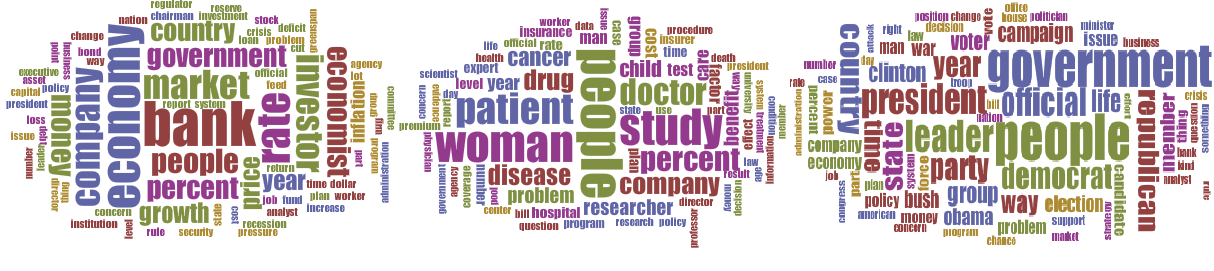
\includegraphics[width=0.70\textwidth]{../images/clouds.png}
            \caption{Key participants in the \emph{Economics}, \emph{Health} and \emph{Politics} subcorpora}
            \label{fig:clouds}
            \end{figure}

            \begin{figure}[htb!]
            \centering
            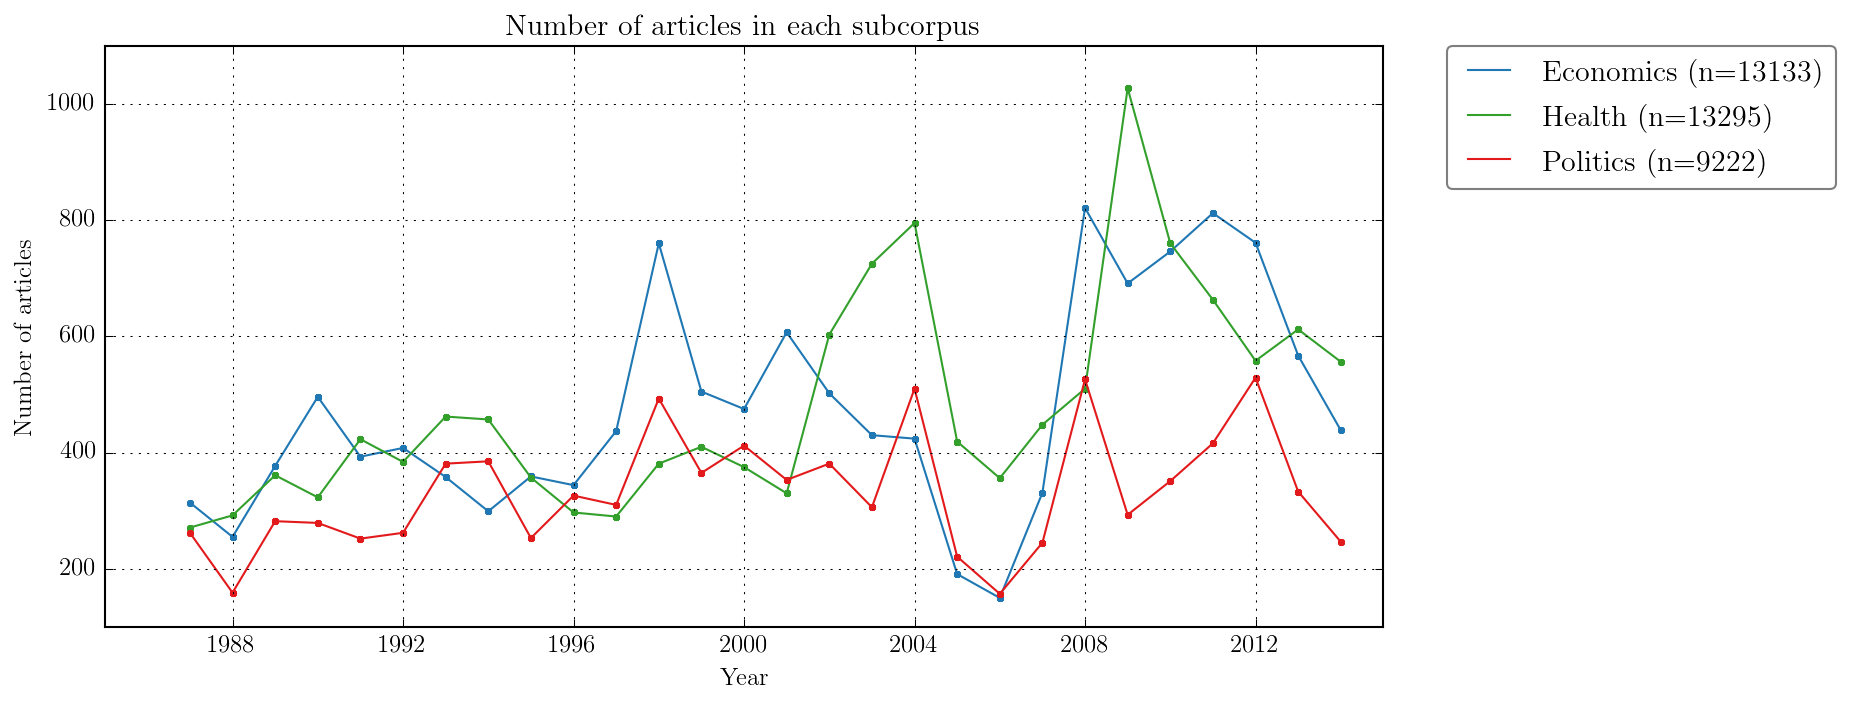
\includegraphics[width=.70\textwidth]{../images/number-of-articles-in-each-subcorpus.png}
            \caption{Number of articles in each subcorpus}
            \label{fig:article_per_subcorpus}
            \end{figure}

            \begin{figure}[htb!]
            \centering
            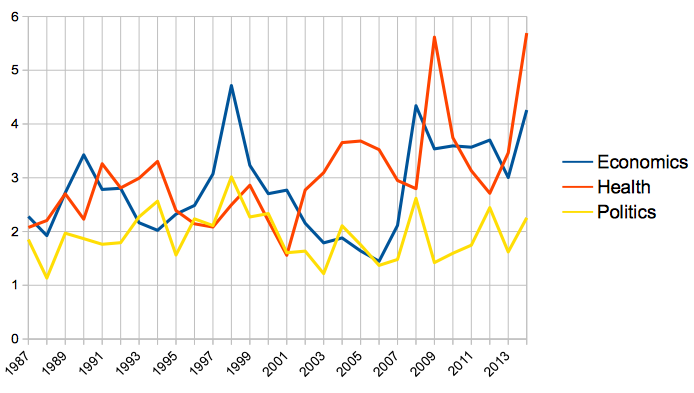
\includegraphics[width=.70\textwidth]{../images/echepol_riskwords.png}
            \caption{Risk words per total number of article topics per year}
            \label{fig:echepol_riskwords}
            \end{figure}
            %
            %Due to time constraints, we restricted the topic comparison to domains that had yielded interesting insights in the earlier interrogations. Further, we found that the smaller size of the subcorpora limited us to lexicogrammatical queries that outputted a large enough number of results for quantitative reliability. Thus, we focussed on the following three areas:

             \begin{table}[htb!]
             \centering
             \small
             \begin{tabular}{|l|l|l|}
                          \hline
                          \textbf{Economics}   & \textbf{Health}         & \textbf{Politics}     \\ \hline
                          political   & high           & political    \\ \hline
                          big         & great          & great        \\ \hline
                          economic    & low            & big          \\ \hline
                          financial   & other          & high         \\ \hline
                          great       & serious        & own          \\ \hline
                          high        & financial      & serious      \\ \hline
                          more        & potential      & new          \\ \hline
                          real        & medical        & real         \\ \hline
                          systemic    & more           & considerable \\ \hline
                          significant & significant    & more         \\ \hline
                          new         & cardiovascular & other        \\ \hline
                          little      & political      & significant  \\ \hline
                          global      & possible       & economic     \\ \hline
                          serious     & small          & financial    \\ \hline
                          other       & real           & potential    \\ \hline
                          excessive   & such           & personal     \\ \hline
                          potential   & genetic        & little       \\ \hline
                          such        & ovarian        & such         \\ \hline
                          much        & same           & public       \\ \hline
                          own         & bad            & military     \\ \hline
                          \end{tabular}
                          \caption{Most common adjectives modifying nominal risks in the topic subcorpora}
                          \label{tab:echepo_adjmod}
             \end{table}

\section{Health}

    Our topic subcorpora were much smaller than our main corpus. As a result, lexicogrammatical querying did not yield quantitatively reliable results. Accordingly, other kinds of corpus linguistic investigation, not reliant on grammatical structure, were applied. 

    First, we considered \emph{keywords}---that is, words that were unusually frequent within the health corpus when compared to the corpus as as a whole.

    Linear regression was used to determine the slope of each keyword's trajectory, and ensure that the p-value of this slope was below 0.05. Results were then sorted into two groups, based on the incline\slash decline of the slope.

    \begin{figure}[htb!]
    \centering
    \begin{minipage}{.48\textwidth}
    \centering
    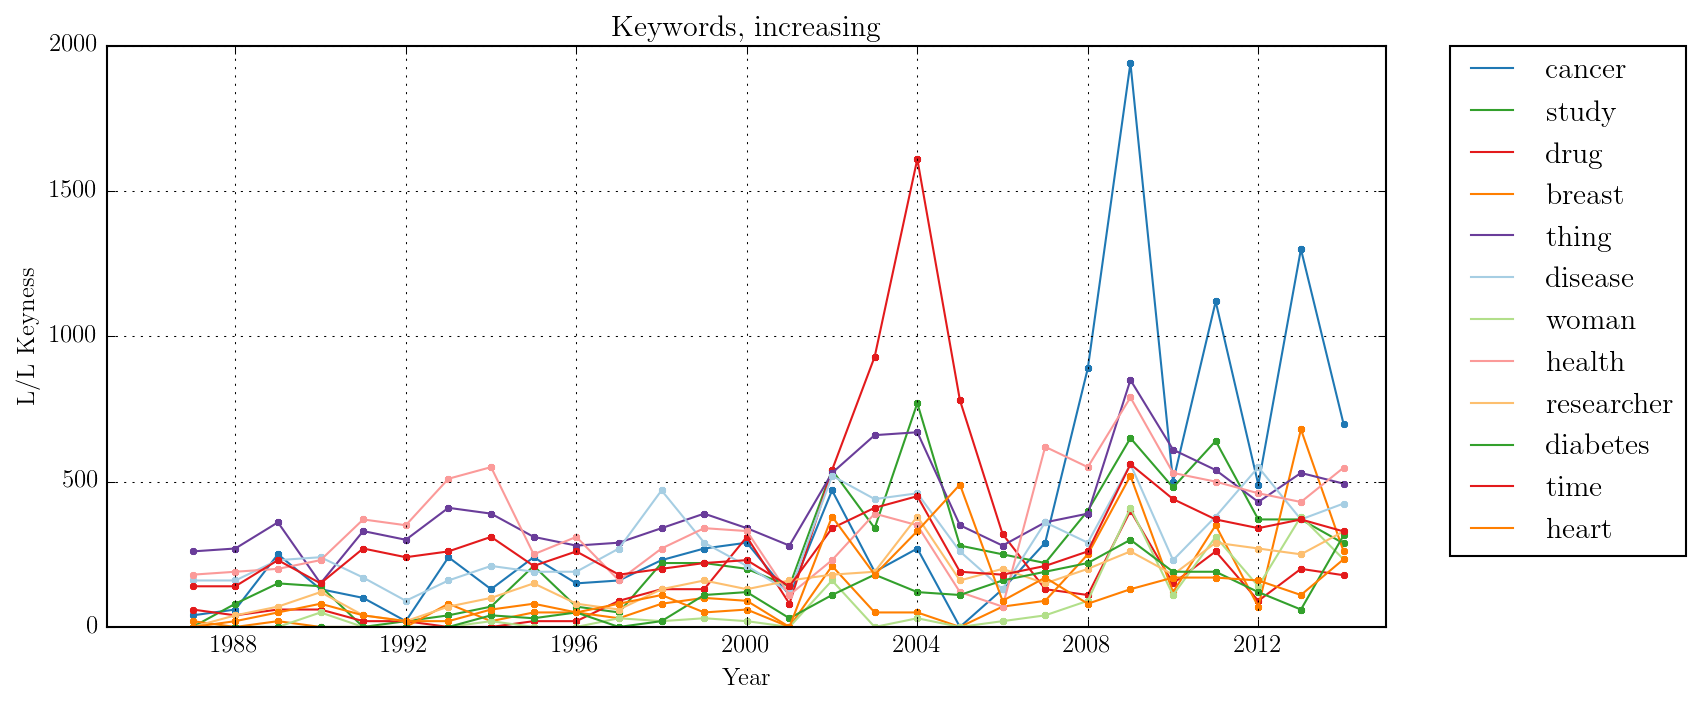
\includegraphics[width=.95\textwidth]{../images/keywords-increasing.png}
    \caption{Keywords becoming more key over time}
    \label{fig:key-inc}
    \end{minipage}%
    \begin{minipage}{.48\textwidth}
    \centering
    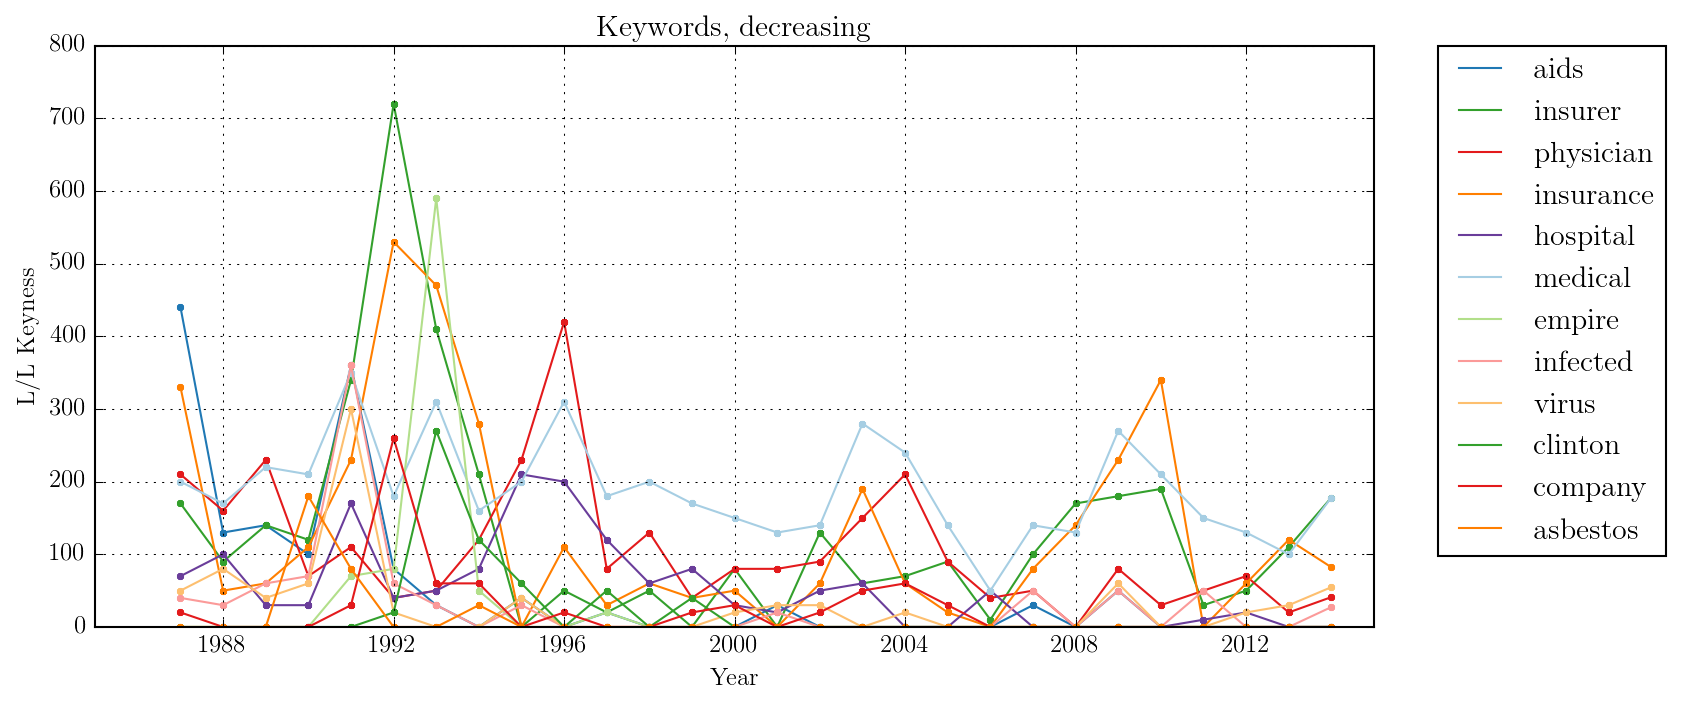
\includegraphics[width=.95\textwidth]{../images/keywords-decreasing.png}
    \caption{Keywords becoming less key over time}
    \label{fig:key-dec}
    \end{minipage}
    \end{figure}

    Next, we were interested in \emph{bigrams}---that is, words that occur beside each other multiple times within a corpus. Bigrams containing a stopword were excluded from analysis, as these results were generally common clusters of closed class words (\emph{in the}, \emph{of a}, \emph{one day}, etc.). Again, linear regression was used to group results into increasing and decreasing groups.

    \noindent
    \begin{figure}[htb!]
    \centering
    \begin{minipage}{.48\textwidth}
    \centering
    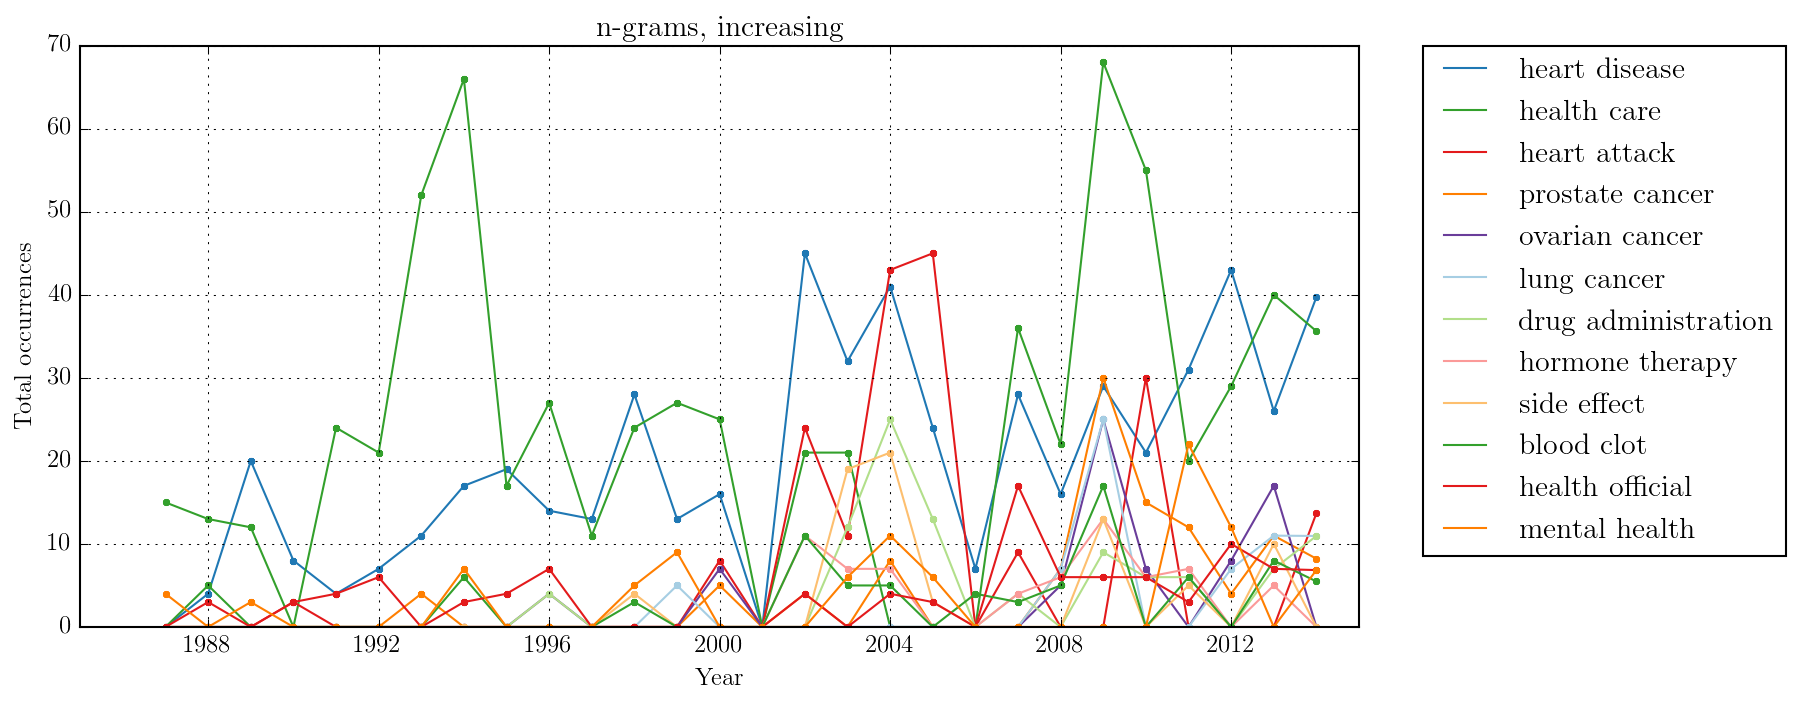
\includegraphics[width=.95\textwidth]{../images/ngrams-increasing.png}
    \caption{bi-grams becoming more frequent over time}
    \label{fig:ngram-inc}
    \end{minipage}%
    \begin{minipage}{.48\textwidth}
    \centering
    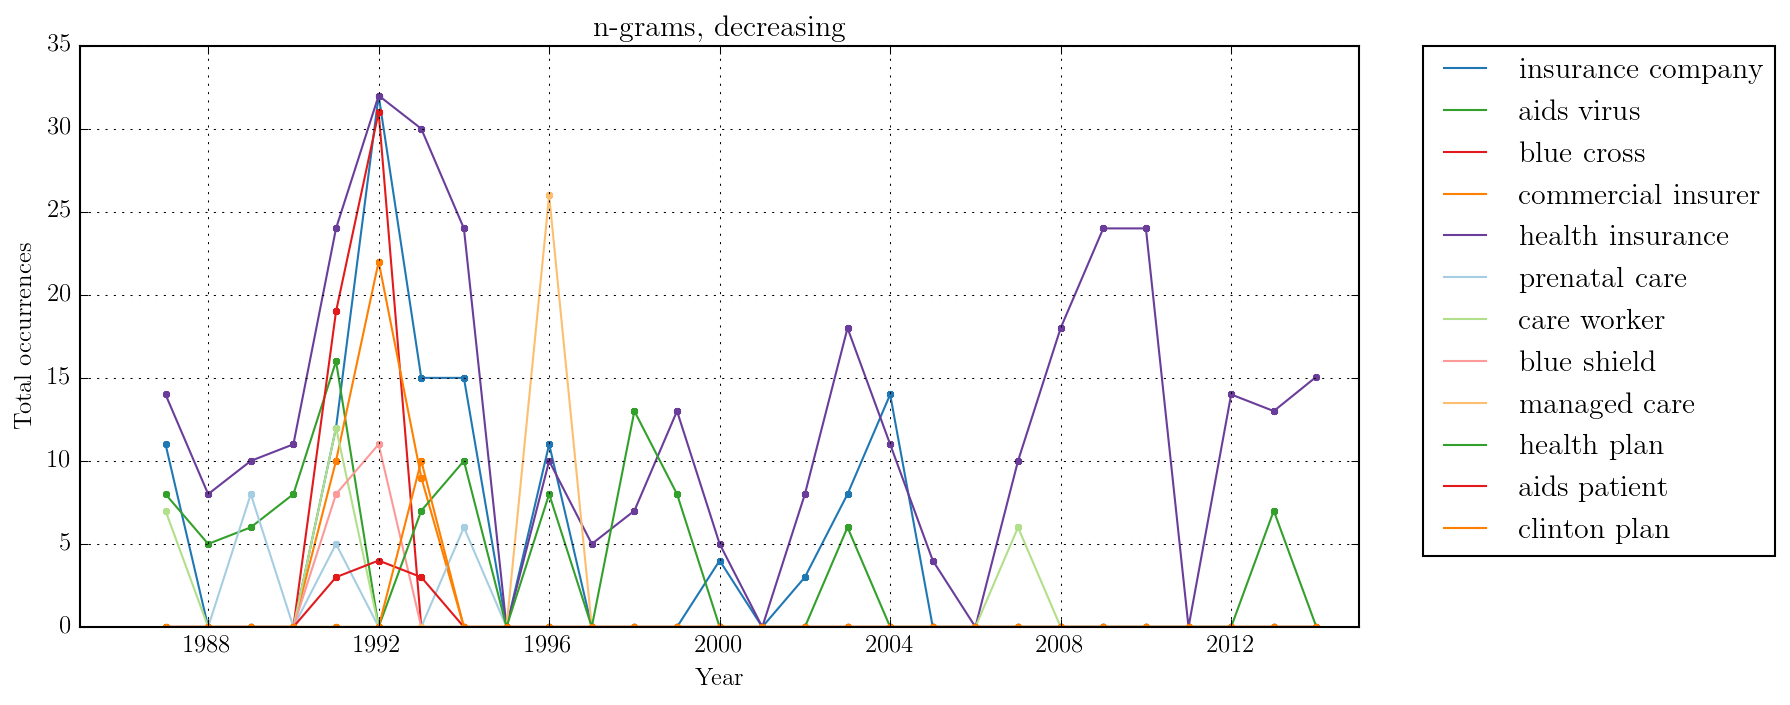
\includegraphics[width=.95\textwidth]{../images/ngrams-decreasing.png}
    \caption{bi-grams becoming less frequent over time}
    \label{fig:ngram-dec}
    \end{minipage}
    \end{figure}

We grouped these into themes, with results entered into one or more categories. Ambiguous results were often concordanced in order to determine the main context of use: \emph{athlete}, for example, could indicate the health condition (\emph{Athlete's foot}), a chain of footwear stores, or denote athletes themselves. The latter was revealed to be by far the most common context, and athlete was thus added to \emph{People, everyday}.

\subsection{Nominal groups in the health subcorpus}

The final part of our investigation of the health subcorpus looked at key nouns or nominal groups. By measuring the slope of trend lines, we could ascertain which groups were becoming more or less common.

    \noindent
    \begin{figure}[htb!]
    \centering
    \begin{minipage}{.48\textwidth}
    \centering
    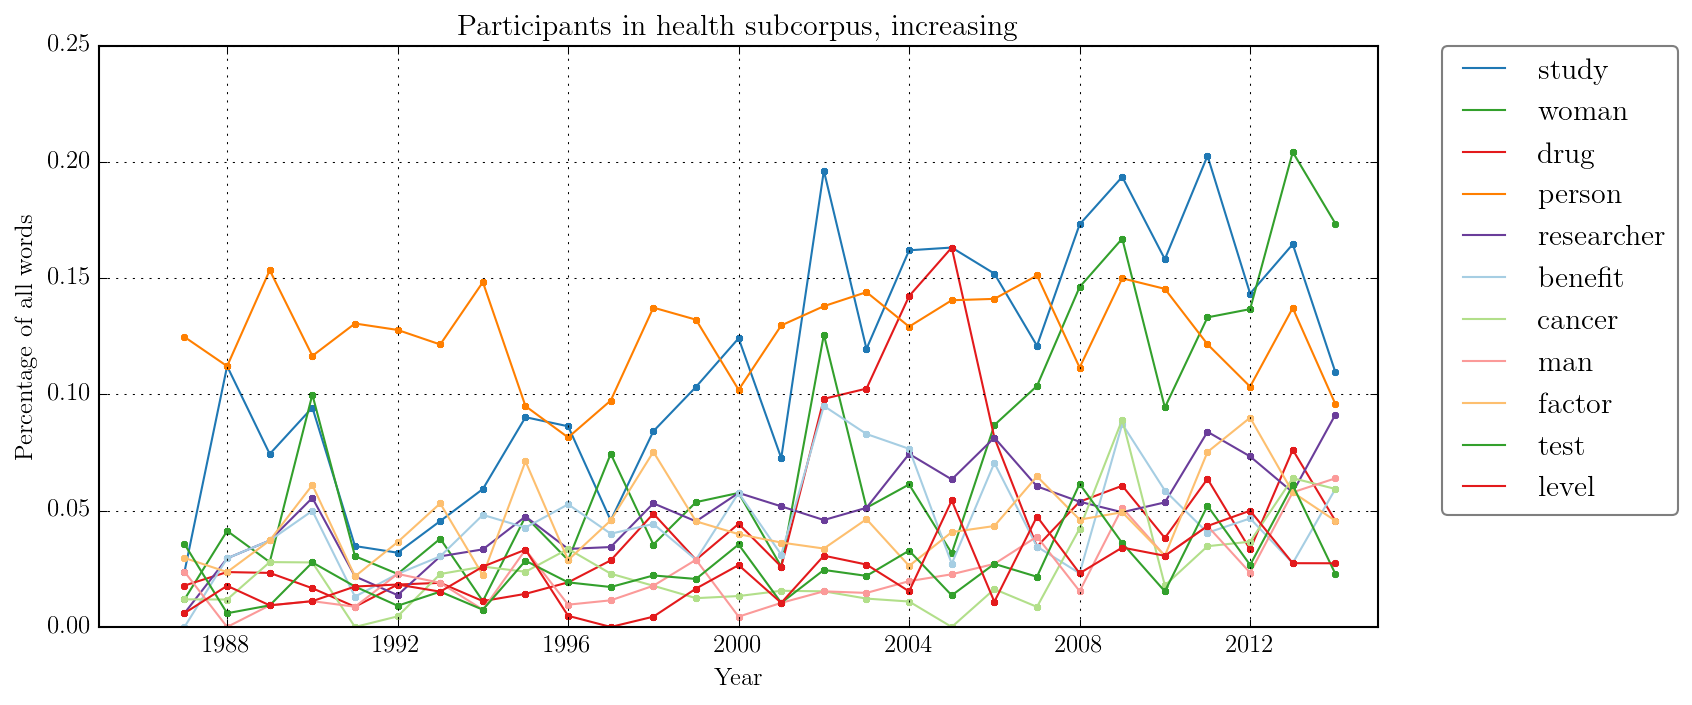
\includegraphics[width=.95\textwidth]{../images/1.png}
    \caption{Absolute frequency of nominal groups becoming more frequent over time}
    \label{fig:1}
    \end{minipage}%
    \begin{minipage}{.48\textwidth}
    \centering
    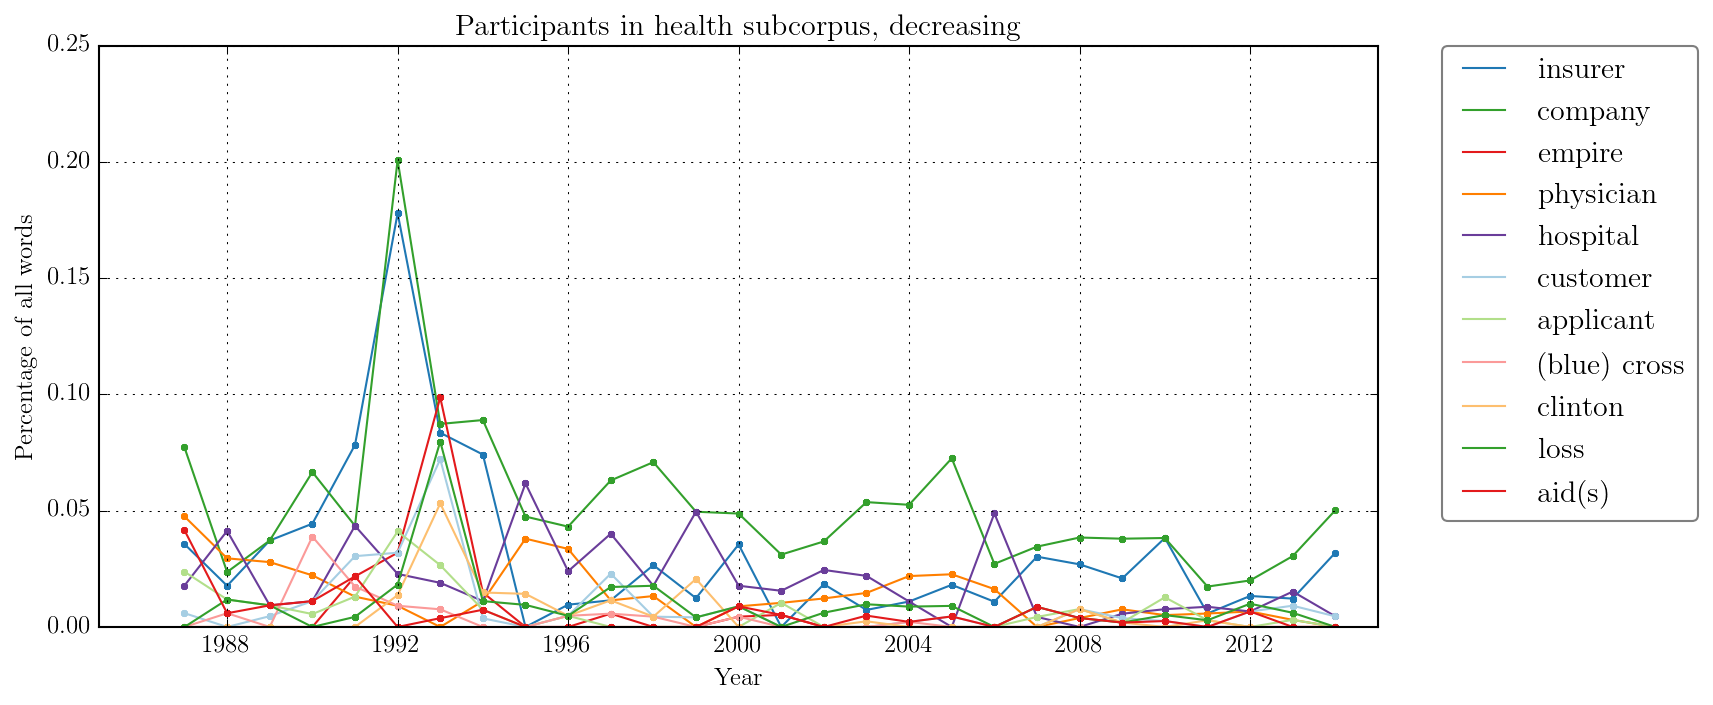
\includegraphics[width=.95\textwidth]{../images/2.png}
    \caption{Relative frequency of nominal groups becoming more frequent over time}
    \label{fig:2}
    \end{minipage}
    \end{figure}
    \noindent
    \begin{figure}[htb!]
    \centering
    \begin{minipage}{.48\textwidth}
    \centering
    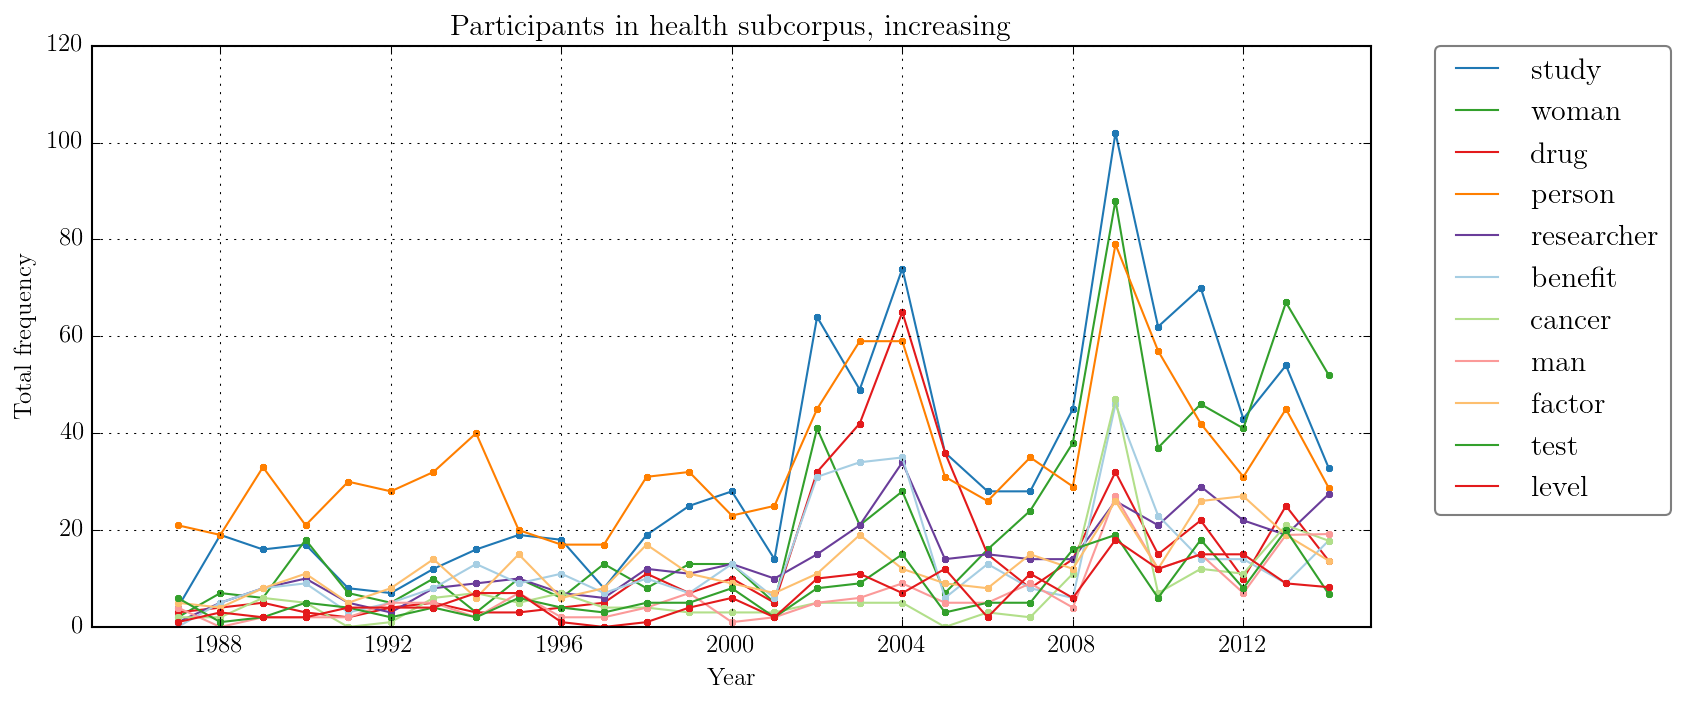
\includegraphics[width=.95\textwidth]{../images/3.png}
    \caption{Relative frequency of nominal groups becoming more frequent over time}
    \label{fig:3}
    \end{minipage}%
    \begin{minipage}{.48\textwidth}
    \centering
    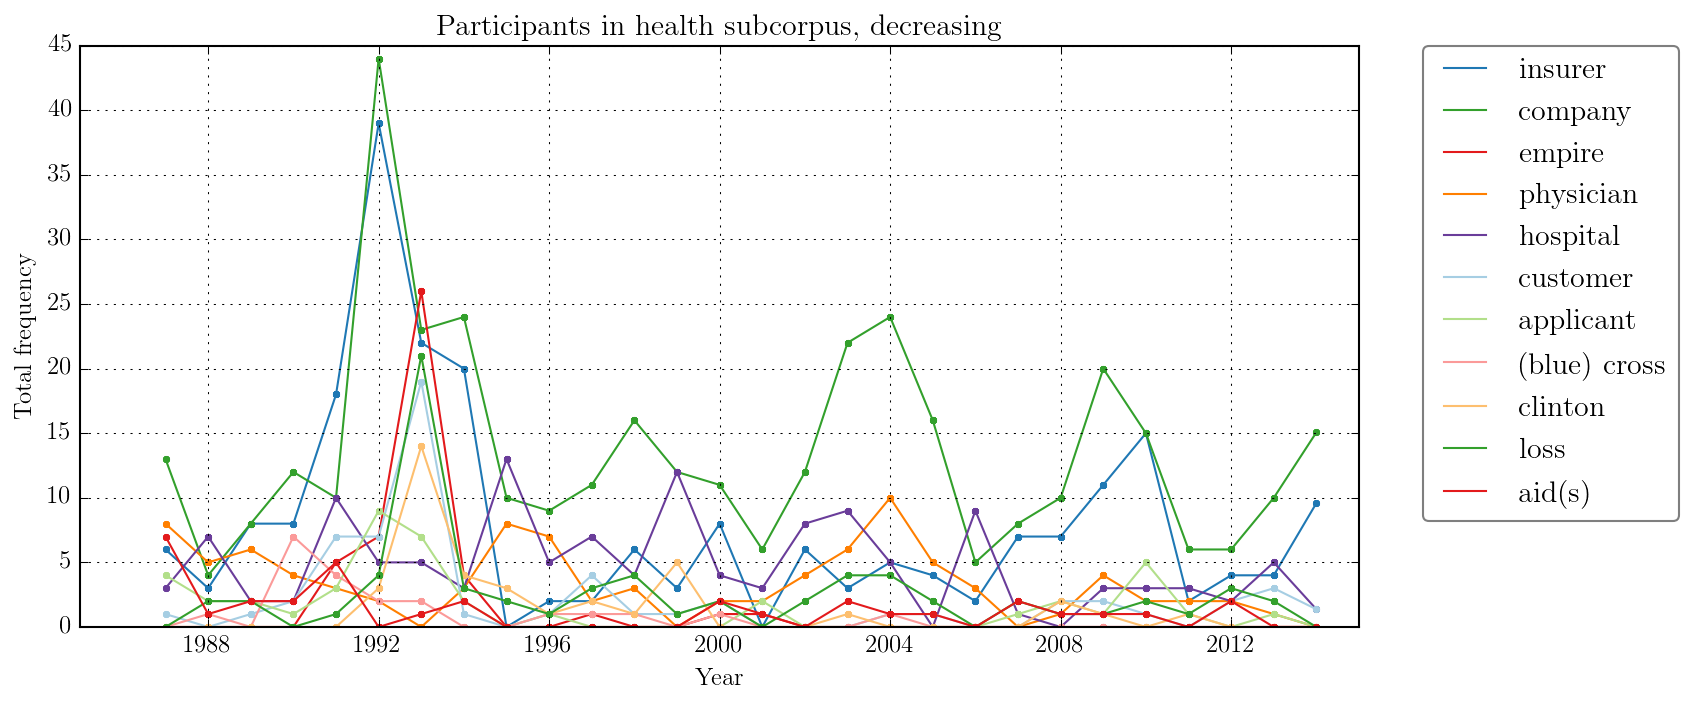
\includegraphics[width=.95\textwidth]{../images/4.png}
    \caption{Relative frequency of nominal groups becoming less frequent over time}
    \label{fig:4}
    \end{minipage}
    \end{figure}

The first major theme that emerges from this interrogation is the shift from infectious to non-infectious disease.

A second point of interest is the decline in terms related to insurance.

Though the prevalence of health insurance in mid 1990s articles was unexpected, as it corresponds with Hillary Clinton's efforts to increase health insurance coverage in the USA, unexpected was the lack of an upswing in insurance terms during the pushes for healthcare reform throughout the Obama administration.

Also apparent is an upward trend for nominal groups related to research (\emph{study, percent, research, etc.}).

This finding was of particular interest, given that the increasing contestation of academic and scientific research are core hypotheses made by Beck.

Concordancing was used to look for evidence of contestation when the nominal groups related to research were instantiated.

\section{Summary}

Broadly speaking, institutional social actors, political representatives and the like appear to have been displaced by individual human actors and components within their everyday life world.

The exception to this rule is research, which

Though further investigation into the emergence of research as a key semantic domain within risk discourse is needed, we hypothesise that it

The increasing commonality of data journalism, where journalists may conduct

Another potential factor is that the exponential increase in academic publications, as well as the increasing ease of access (via the web) has made reporting of 

This may also be a part of the increase in health risk discourse as well.

The lack of contestation points to an area in which Beck's conceptualisation of risk in late modernity may be at odds




\section{Issues in the health corpus investigation}

The first major issue was the smaller size of the corpus, which necessitated different kinds of analysis.

Within keywording and ngramming, it became clear that broader linguistic change and specific events are difficult to separate.

This, however, is where we can see the clearest examples of the link between events and language change. Interspersed throughout the keywords and n-grams are terms ranging in specificity. It is through categorisation of these varying levels that we can smooth out the 

The keywording in particular revealed a number of ambiguities. A more reliable\slash systematic method for grouping keywords would ameliorate this concern.

\section{Summary}

    The smaller size of topic subcorpora necessitated different kinds of analysis. Fortunately, such methods are well documented within corpus assisted discourse studies. Following on from these methodologies, we located particularly frequent terms, and analysed them in their context of use.

    % analysis here

    Ultimately, the ways in which a corpus can be analysed are dependent on the size of the corpus. 


%Comparing the behaviour of risk words in three smaller corpora is complicated by the lack of existing methodologies.

\afterpage{%
\begin{table}
\centering
\tiny
\begin{tabular}{|lrcl|}
\hline
1 & We know this now because                           & researchers & tested both theories , side by side , to see which \\
2 & something the public did not : Yale University     & researchers & had tentatively concluded that PPA was linked to a \\
3 & Instead ,                                          & researchers & say , young killers must be seen as extremely      \\
4 & of men with E.D. , or at risk for developing it ,  & researchers & in Italy found that the men could improve their    \\
5 & If you were an academic                            & researcher  & , you 'd have to persuade your institutional       \\
6 & Some                                               & researchers & believe hyperthymics may be at increased risk of   \\
7 & index , smoking and several other risk factors ,   & researchers & found that women on postmenopausal hormone therapy \\
8 & will have public health consequences , the         & researchers & said                                               \\
9 & Finally , and perhaps most powerfully ,            & researchers & say that a life in poverty is a life of stress     \\
10 & Office of Protection from Research Risks said the  & researchers & altered the medical records of patients , then     \\
11 & In their paper , the                               & researchers & noted that `` countries in which wine is the       \\
12 & In another study , by                              & researchers & at the University of Connecticut , leg strength    \\
13 & In an unexpected finding , the                     & researchers & reported that the women receiving goserelin also   \\
14 & that , far from protecting the heart as many       & researchers & had assumed , the therapy may have put the women   \\
15 & Now                                                & researchers & have found that elevated risk of psychiatric       \\
16 & of a New York Fire Department rescue company and a & researcher  & who is exploring the psychological bases of        \\
17 & Department of Veterans Affairs said the California & researchers & did not properly assess the safety of experimental \\
18 & Other                                              & researchers & , working with similar kinds of data , have        \\
19 & The                                                & researchers & concluded that the study '' provides the first     \\
20 & On the other hand , said Dr. Susan Czajkowski , a  & researcher  & at the National Heart , Lung and Blood Institute   \\
21 & exactly how a given AIDS patient was infected ,    & researchers & do not know exactly how much the risk of           \\
22 & In an effort to finance debts , '' the             & researchers & said , `` ordinary people are paying the ultimate  \\
23 & during the next 25 years of about 6 percent , the  & researchers & found                                              \\
24 & To obtain consent ,                                & researchers & are required to explain that the experiments are   \\
25 & slightly increasing their risks of dying earlier , & researchers & reported yesterday                                 \\
26 & Utah                                               & researchers & have videotaped 150 couples to measure the effect  \\
27 & blood cells -- became patients ' property ,        & researchers & taking them without detailed consent and explicit  \\
28 & In mapping the human genome ,                      & researchers & determined that nearly 99 percent of genetic       \\
29 & The                                                & researchers & were unable to include family history of diabetes  \\
30 & of Internal Medicine , Dr. Solomon and other       & researchers & looked at the comparative risks posed by different \\
31 & the perception of risk , said Pete Delaney , a     & researcher  & with the administration , adding that only about 9 \\
32 & The                                                & researchers & conclude that irregular sleep by itself may be a   \\
33 & Dr. Bernard H. Fox , a federal                     & researcher  & who became a pioneer in investigating the effect   \\
34 & The                                                & researchers & said it was unclear why smoking appeared to        \\
35 & The Stanford                                       & researchers & , who included Dr. Irving Weissman , a leading     \\
36 & But                                                & researchers & like Dr. Monahan and Dr. McNiel are applying       \\
37 & A study of 1,240 people by                         & researchers & at Case Western Reserve University in Cleveland    \\
38 & that of diabetes , '' said Dr. Steven G. Deeks , a & researcher  & at the University of California , San Francisco    \\
39 & In addition ,                                      & researchers & hope that the studies linking the disorder to      \\
40 & night on WNBC-TV , that Cornell University         & researchers & have found a risk of alcoholism among New York     \\
41 & , suggesting chance could play a role , but        & researchers & say the trends are credible because they are       \\
42 & The                                                & researchers & also found that patients became significantly less \\
43 & Over all ,                                         & researchers & found that calcium supplements did not lower the   \\
44 & of the power AIDS activists have mustered to push  & researchers & to do experiments that many experts deem foolish   \\
45 & The                                                & researchers & next study the extent to which medical treatment   \\
46 & was the fourth-leading risk factor for death , the & researchers & said                                               \\
47 & study 's author , Kathleen Miller , an addiction   & researcher  & at the University of Buffalo , says it suggests    \\
48 & The                                                & researchers & claim that the benefits of the research -- greater \\
49 & Some                                               & researchers & suspect genetics : Maybe thin people who develop   \\
50 & Dr. Bishop and Dr. Varmus , along with other       & researchers & , have found that the genes can cause cancer in    \\
51 & Finally ,                                          & researchers & at Tufts reported last month in The Journal of     \\
52 & The lead                                           & researcher  & , Dr. Tina V. Hartert , director of the Center for \\
53 & harmful cholesterol in the blood , even when the   & researchers & accounted for other risk factors for high          \\
54 & on cases stemming from the Sept. 11 attacks ,      & researchers & found that the more deeply therapists were         \\
55 & The                                                & researchers & did find an increased risk of other , less common  \\
56 & The inquiry in Ms. Wan 's case found that          & researchers & had adequately explained the risks to her and that \\
57 & For example , she said ,                           & researchers & are experimenting with fast-growing carp that      \\
58 & than 23,000 Greek men and women ages 20 to 86 ,    & researchers & found that napping at least three times a week for \\
59 & precision afforded by simple computing devices ,   & researchers & say , promise to deliver new insights on risk      \\
60 & only two categories of risk , minimal and great ,  & researchers & were often discouraged from doing research         \\
61 & the clear advantage of moderate drinking , the     & researchers & presented their findings with strong caveats       \\
62 & As the genes become better understood ,            & researchers & expect to find ways to block them if they become   \\
63 & adolescents followed over a period of nine years , & researchers & at the New York Psychiatric Institute found that   \\
64 & Health , for example , said that 100 psychiatric   & researchers & gathered in a room would all probably agree that   \\
65 & smoking might have damaged the fathers ' sperm ,   & researchers & said yesterday                                     \\
66 & with 20 percent of the control group , the         & researchers & found                                              \\
67 & The                                                & researchers & found that for each four-inch increase in height   \\
68 & between height and cancer may help guide           & researchers & to study hormones and growth factors that          \\
69 & Why do                                             & researchers & and willing patients test the boundaries of        \\
70 & 's disease as those who have never smoked ,        & researchers & say , and several small studies have indicated     \\
71 & But                                                & researchers & said they had never seen this before , either in   \\
72 & In 2012 , British                                  & researchers & , by combining results from clinical trials that   \\
73 & After adjusting for various health factors , the   & researchers & found that for each increase of 10 micrograms per  \\
74 & The F.D.A. has asked                               & researchers & at Columbia to reclassify the cases of self-harm   \\
75 & The                                                & researchers & said this was troubling , given recent studies     \\
76 &  A large team of                                    & researchers & , led by V. Wendy Setiawan , an assistant          \\
77 &  and violated Federal regulations because the       & researchers & had not informed patients of the risks             \\
78 &  Yet                                                & researchers & also concluded the risk of stroke was the same as  \\
79 &  In 2002 ,                                          & researchers & halted the largest clinical trial ever conducted   \\
80 &  , and while they might not be surprising to        & researchers & , they were intended to inform the public as well  \\
81 &  Many                                               & researchers & said anger-prone people could reduce the risk of   \\
82 &  Using preserved blood samples of pregnant women ,  & researchers & have found that low vitamin D levels are           \\
83 &  And so now                                         & researchers & have been working on new strategies : Developing   \\
84 &  This month , Danish                                & researchers & reported on a 15-year study of 12,000 nurses       \\
85 &  She said                                           & researchers & thought older medicine was riskier because the     \\
86 &  Last Sunday ,                                      & researchers & released data that showed that outdoor air         \\
87 &  But when the company and the                       & researcher  & are one and the same , he said , that check is     \\
88 &  Huntington 's disease and cystic fibrosis , and    & researchers & say tests identifying those at high risk of heart  \\
89 &  may increase with a father 's advancing age ,      & researchers & reported yesterday                                 \\
90 &  Denise Juliano-Bult , a                            & researcher  & at the National Institute of Mental Health , said  \\
91 &  those who gain fat around the hips and thighs ,    & researchers & say                                                \\
92 &  in the British Medical Journal in August ,         & researchers & in Argentina showed that women who were given      \\
93 &  Next ,                                             & researchers & said , they want to do a large study like one      \\
94 &  The                                                & researchers & noted that the drinks contain high levels of       \\
95 &  The                                                & researchers & offered some other examples of how the risks       \\
96 &  Some other                                         & researchers & questioned the findings , and most agreed that the \\
97 &  For purposes of comparison , the                   & researchers & also examined inherited variations in 13 genes     \\
98 &  And the flaws are compounded , the                 & researchers & said , when journalists do n't report the context  \\
99 &  A few years ago , Mercedes Carnethon , a diabetes  & researcher  & at the Feinberg School of Medicine at Northwestern \\
100 &  As with beta carotene ,                            & researchers & were shocked                                       \\
\hline
\end{tabular}
\caption{100 random instances of \emph{researcher} in the health subcorpus}
\label{tab:research}
\end{table}
\clearpage
} % Limitations, research agenda, conclusions

%end matter

    \cleardoublepage
    \singlespacing
    %\footnotesize
    \printendnotes
    \cleardoublepage
    \singlespacing
    \bibliographystyle{apacite}
    \bibliography{references/references}
    \cleardoublepage

    \end{document}






















\section{New approaches to risk research}

Our methodology involves combining \emph{corpus assisted discourse studies} with \emph{systemic functional linguistics} in order to understand how risk words are used in the NYT, and how usage has changed within the sampled period.

\subsection{Corpus-assisted discourse studies}

Text corpora---that is, large bodies of digitised, well-structured text---are not unknown to risk researchers.

Since their work, however, enormous strides have been taken in the field of corpus-assisted discourse studies, as well as in computational fields such as natural language processing, which provide means of annotating language with grammatical information, and querying the annotated texts in complex ways.

It is also more and more feasible to build particular corpora for particular investigations, rather than relying on general corpora, comprised of diverse kinds of texts.

\subsection{Functional linguistics}

    Central to any well-considered study of language use is a theory of language, which may either implicitly or explicitly inform the kinds of analyses being done. A number of frameworks exist for connecting lexis and grammar to functional meanings. Notable within risk research has been frame semantics, which has been used to categorise different risk frames and their constituents \cite{fillmore_toward_1992}. One such framework is \emph{systemic functional linguistics} \cite<see>{halliday_introduction_2004}, which conceptualises language as a \emph{sign system} that is employed by users in order to achieve \emph{social functions}. This theory explicitly underlies our investigation.

    We use SFL for three main reasons. First, it is the most detailed functional grammar \cite{eggins_analysing_2004}: when compared with frame semantics, it provides a more rigorous description of how risk can behave \emph{lexicogrammatically}---that is, in relation to both other words and grammatical features---within a clause. This makes it possible to search parsed texts in nuanced ways. Second, it is a functional-semantic theory, rather than a cognitive-semantic one. While the remarkable achievement of frame semantics is its mapping out of cognitive frames, we are largely unable to operationalise these with our dataset, as we have little information regarding the specific interactants (writers and readers) of the original texts. Moreover, cognitive understandings of text are complicated in situations where the text's author is producing the text within an institutional context, for a readership. Without downplaying the potential importance of cognitivist accounts of risk, we have instead opted here to focus on risk words as \emph{instantiations of parts of the linguistic system for the purposes of meaning-making}, rather than as a \emph{representation of the cognitive schemata that underlie our behaviour}.

    The third benefit of SFL is that it provides not only a grammar, but a a conceptualisation of the relationship between text and context. A foundational tenet of SFL, and a point of departure from other linguistic theories, is the notion that we can create a description of context based \emph{solely} on the lexicogrammatical content of the text. This is particularly suitable for us, given that our texts arrived to us abstracted from their original contexts. This context was then further obscured through the parsing process. As such, SFL provides an ability to account for discourse-semantics using corpora that other theories cannot.


%\section{Outcomes of the study}

%Our project makes significant contributions to both sociological theory and digital humanities methodology.











